\documentclass[10pt, a4paper, titlepage]{article}
\usepackage[margin=1in]{geometry}
\usepackage{graphicx, latexsym}
\usepackage{titling}
\setlength{\droptitle}{-25em}
\renewcommand{\maketitlehooka}{\Large}
\usepackage{setspace}
\usepackage{amssymb, amsmath, amsthm}
\usepackage[export]{adjustbox}
\usepackage{bm}
\usepackage{wrapfig}
\usepackage{epstopdf}
\usepackage{microtype}
\usepackage[hidelinks]{hyperref}
\usepackage{titling}
\usepackage{multirow}
\usepackage[labelfont=bf]{caption}
\captionsetup{format=hang,justification=raggedright,singlelinecheck=false}
\usepackage[table,xcdraw]{xcolor}
\usepackage{colortbl}
\usepackage{lscape}
\usepackage{float}
\usepackage[sort&compress,round,semicolon,authoryear]{natbib}
\usepackage{bookmark}
\usepackage{listings}
\usepackage{xcolor}
\definecolor{codegreen}{rgb}{0,0.6,0}
\definecolor{codegray}{rgb}{0.5,0.5,0.5}
\definecolor{codepurple}{rgb}{0.58,0,0.82}
\definecolor{backcolour}{rgb}{1,1,1}
\lstdefinestyle{mystyle}{
    backgroundcolor=\color{backcolour},   
    commentstyle=\color{codegreen},
    keywordstyle=\color{magenta},
    numberstyle=\tiny\color{codegray},
    stringstyle=\color{codepurple},
    basicstyle=\ttfamily\footnotesize,
    breakatwhitespace=false,         
    breaklines=true,    captionpos=t,                    
    keepspaces=true, numbers=left,                    
    numbersep=5pt, showspaces=false,                
    showstringspaces=false, showtabs=false, tabsize=2}
\lstset{style=mystyle}
\hypersetup{
    pdftitle={Master Thesis Heleen Brüggen},
    pdfauthor={Heleen Brüggen},
    pdfsubject={Master Thesis Heleen Brüggen},
    pdfkeywords={},
    bookmarksnumbered=true,
    bookmarksopen=true,
    bookmarksopenlevel=1,
    colorlinks=false,
    pdfstartview=Fit,
    pdfpagemode=UseNone
}

\singlespacing%

\begin{document}
\begin{titlingpage}
\begin{center}
\Huge\textbf{Master Thesis:  \\ Multilevel Multivariate Imputation by Chained Equations through Bayesian Additive Regression Trees} \\
\Large\textit{Methodology and Statistics for the Behavioural, Biomedical and Social Sciences}

\vspace{.5cm}

\normalsize\textit{Heleen Brüggen}

% \vspace{11.5cm}
\vspace{1cm}

\begin{minipage}{1\textwidth}
\begin{center}
\section*{Abstract}
\end{center}
\end{minipage}

\vspace{.25cm}

\begin{minipage}{1\textwidth}
    This study investigates whether the use of multilevel Bayesian Additive Regression Trees (BART) in a multilevel multiple imputation context improves the bias, coverage, and variance estimates of the multilevel model parameter estimates compared to current practices. At present, defining a congenial imputation model for a hierarchically structured dataset is an laborious process due to complicated non-linear relationships. Using a non-parametric, tree-based BART model as the imputation model might alleviate these complexities. A simulation study was conducted to evaluate the performance of multilevel BART models in a multilevel imputation context. The population data-generating mechanism was based on a multilevel linear model with random intercepts, slopes, and cross-level interactions. The performance of multilevel BART models was compared to single-level predictive mean matching (PMM), multilevel PMM, single-level BART and complete case analysis. The results show that the multilevel PMM model performed best in terms of bias, variance, and coverage of the parameter estimates. However, the multilevel BART model showed promising results for the random intercepts and slopes. So, in its current form, multilevel BART models do not offer an improvement over the existing implementation.
\end{minipage}

\vspace{4cm}

\begin{minipage}{.5\textwidth}
\begin{center}
            
\includegraphics[width=10cm]{graphs/UU_logo_2021_EN_RGB.png}
\end{center}
\end{minipage}%
    
\vspace{.25cm}

\begin{minipage}{0.5\textwidth}
\begin{flushleft}

\textbf{Word count:} \\
\textbf{Candidate Journal:} \\
\textbf{FETC Case Number:} \\
\textbf{Research Archive:} \\
\textbf{Supervisors:} \\
T. Volker MSc. \\
Dr. G. Vink \\
H. Oberman MSc.
\end{flushleft}
\end{minipage}%
\begin{minipage}{0.5\textwidth}
\begin{flushright}

6450 \\ %detex thesis/Thesis_Heleen_Brueggen.tex | wc -w
Computational Statistics \& Data Analysis \\
23-1778 \\
\url{github.com/heleenbrueggen/masterthesis} \\
------------------------\\
Utrecht University \\
Utrecht University \\
Utrecht University
\end{flushright}
\end{minipage}

\end{center}
\end{titlingpage}

\newpage
\tableofcontents
\newpage
\section{Introduction}
Incomplete data is a common challenge in many fields of research. Frequently used ad hoc strategies to deal with missing data, such as complete case analysis or mean imputation, often lead to erroneous inferences in realistic situations. Missingness can follow a multivariate mechanism that may depend on observed data or even unobserved data, leading to biased estimates and inaccurate variance estimates when using one of these ad hoc strategies \citep{buurenFlexibleImputationMissing2018, kang2013, enders2017, austin2021, little2002}. Multiple imputation (MI;~\Citealp{rubin1987}) is proven to be an effective method for dealing with multivariate incomplete data supported by a considerable amount of methodological research \citep{mistlerComparisonJointModel2017, buurenFlexibleImputationMissing2018, enders2017, burgette2010, austin2021, audigier2018, vanbuuren2007, grund2021, hughes2014, little2002}.
% Rubin defined three of such missing data mechanisms: Missing Completely At Random (MCAR) where the cause of the missing data is unrelated to the data, Missing At Random (MAR) where the missing data is related to the observed data, and Missing Not At Random (MNAR) where the missing data may also be related to unobserved data \citep{rubin1976}.

MI separates the missing data problem from the analysis problem \citep{mistlerComparisonJointModel2017, buurenFlexibleImputationMissing2018, enders2017, burgette2010, austin2021, audigier2018, vanbuuren2007, grund2021, hughes2014, little2002, carpenter2013, bartlett2015}. A statistical model specifying the variables used for imputation, i.e. the imputation model, is defined for every variable with missing values. Each missing value in the dataset is imputed \textit{m} times by drawing values from their posterior predictive distribution conditional on the observed data and parameters from the imputation model. By repeatedly drawing values from the posterior predicitve distributions --- in other words, the distribution of plausible replacement values --- the necessary variation associated with the missingness problem is considered. After imputation, each of the imputed datasets are analyzed according to the model of interest, i.e. the substantive analysis model. Then, their \textit{m} corresponding model parameters are pooled together according to Rubin's rules \citep{rubin1987}. 
% \citep{buurenFlexibleImputationMissing2018, austin2021, carpenter2013,enders2017}. 
One central requirement for MI is the concept of congeniality; the imputation model should should be at least as general as the analysis model and preferably all-encompassing \citep{grund2018, enders2018, meng1994multiple, bartlett2015, grund2016, little2002}. If not, the imputation model will not be compatible with the analysis model and the pooled estimates of the latter may be biased. 

% So, when the complexity of data increases, specifying the imputation models becomes more difficult \citep{grund2018, buurenFlexibleImputationMissing2018}.
When MI is applied in a multilevel data context, concerns regarding the concept of congeniality become more pronounced \citep{mistlerComparisonJointModel2017, enders2018, enders2018a, enders2020, buurenFlexibleImputationMissing2018, taljaard2008, enders2016, resche-rigon2018, audigier2018, dong2023, grund2016, grund2018a, grund2018, ludtke2017, grund2021, quartagno2022}. Multilevel data is hierarchically structured, where, for example, students are nested within classes within schools or patients within hospitals \citep{hox2017, hox2011}. When analyzing multilevel data, this hierarchical structure should be taken into consideration. Ignoring it will underestimate the intra-class correlation (ICC) and standard errors, as conventional statistical analyses assume independence of observations \citep{buurenFlexibleImputationMissing2018, ludtke2017, taljaard2008, hox2011}. The ICC can be interpreted as the proportion of the total variance at level-2 \citep{gulliford2005, shieh2012, hox2011}. Accounting for this structure, can be done using multilevel models (MLMs; \Citealp{hox2017, hox2011, ludtke2017}). MLMs can contain variables relating to the individual level --- level-1 variables --- or to the grouping structure --- level-2 variables or potentially higher order structures. For example, imagine a case where students are nested within classes. Here, the academic performance of a student is a level-1 variable, whereas the teacher's experience is a level-2 variable. Additionally, MLMs allow you to specify random intercepts, indicating that some classes have students that significantly perform better or worse academically on average; random slopes, indicating that the relationship between the performance of students and the outcome variable differs between classes; and cross-level interactions, indicating that the effect of performance of students can differ with the teacher's experience \citep{hox2017, hox2011}. Typically, the complexity of the multilevel analysis model is built step-wise with non-linearities, meaning the analysis model is not determined beforehand: predictors, random intercepts, random slopes, and cross-level interactions are added in a stepwise manner to the model \citep{hox2017, hox2011}. Thus, ensuring congeniality for the imputation model can be complex, since the final analysis model is not pre-determined. Furthermore, including the hierarchical structure along with cross-level interactions or other complicated non-linearities in imputation models is quite challenging \citep{buurenFlexibleImputationMissing2018, burgette2010, hox2011}, also because very complex models might not converge \citep{buurenFlexibleImputationMissing2018}.

A popular and flexible implementation of MI in a multilevel context, is fully conditional specification (FCS), otherwise known as chained equations \citep{audigier2018, burgette2010, vanbuuren2007, grund2018a}. FCS employs univariate linear mixed models to account for the hierarchical structure of multilevel models \citep{mistlerComparisonJointModel2017, enders2018, resche-rigon2018} and iteratively imputes each incomplete variable conditional on observed and previously imputed variables \citep{mistlerComparisonJointModel2017, buurenFlexibleImputationMissing2018, enders2016, enders2018, enders2018a, hughes2014, grund2018a}. Furthermore, it can impute non-linearities, such as cross-level interactions, by using `passive imputation` or defining a separate imputation model for the non-linearities \citep{buurenFlexibleImputationMissing2018, grund2018}. However, including these non-linearities in FCS is still very complicated \citep{grund2021, grund2018,buurenFlexibleImputationMissing2018}. FCS can also handle random intercepts and slopes, yet, once again, correctly specifying an imputation model accounting for these random effects can be challenging \citep{grund2021, grund2018,buurenFlexibleImputationMissing2018}.

%  and, thus, researchers' focus has predominantly been on the inclusion of random intercepts and slopes, but not of cross-level interactions \citep{grund2018a, grund2016, enders2018, enders2018a, enders2020, enders2016}.

Non-parametric, tree-based models might alleviate these complexities when defining imputation models. They do not assume a specific data distribution. So, they implicitly model non-linear relationships and can simultanously handle continuous and categorical variables \citep{hill2020, burgette2010, lin2019, chipman2010, james2021, salditt2023, breiman1984}. Studies showed that the use of tree-based, non-parametric models like regression trees, random forests, or Bayesian Additive Regression Trees (BART) in imputation of single-level data simplified the imputation process \citep{burgette2010,xu2016,silva2022,waljee2013}. They showed better model parameter estimates than parametric methods. Specifically, the imputations showed better confidence interval coverage of the parameters, lower variance and lower bias, especially in non-linear and interactive contexts \citep{burgette2010, xu2016, silva2022}. \citet{waljee2013} also found lower missclassification error rate for the predicted class as well as lower imputation error when imputing with a random forest algorithm compared to multivariate imputation by chained equations (\texttt{mice}) using linear, logistic, and polytomous logistic regression imputation models, K-nearest neighbors (KNN) and mean imputation.

In prediction, multilevel-BART models have predominantly been implemented with random intercepts only \citep{chen2020, wagner2020, tan2016, wundervald2022}. \citet{wagner2020} have found that this random intercept R-BART model provided better predictions with a lower mean squared error (MSE) compared to a parametric MLM, \citet{tan2016} found higher area under the curve (AUC) values compared to a singel-level BART model and linear logistic random intercept model, and \citet{chen2020} found better predictions and better coverage of the parameter estimates compared to parametric models and a single-level BART model. Other researchers modeled the random intercept as an extra split on each terminal node and found a lower MSE compared to a standard BART model and parametric MLMs \citep{wundervald2022}.~\citet{dorie2022} developed a multilevel BART model that included random intercepts, random slopes and cross-level interactions by modeling these random parts with a Stan \citep{lee2017} model and the fixed parts with a BART model. Their results showed that their algorithm \texttt{stan4bart} showed better coverage of the population values and lower root mean squared error (RMSE) compared to BART models with varying intercept, BART models ignoring the multilevel structure, bayesian causal forests, and parametric MLMs. 

% BART models have been implemented in a multilevel prediction context. However, multilevel-BART models (M-BART) have predominantly been implemented with only random intercepts \citep{chen2020, wagner2020, tan2016, wundervald2022}. In a prediction context, 

% \citet{wagner2020} have found that this random intercept M-BART model provided better predictions with a lower mean squared error (MSE) compared to a parametric MLM, \citet{tan2016} found higher area under the curve (AUC) values compared to a singel-level BART model and linear random intercept model, and \citet{chen2020} found better predictions and better coverage of the estimates compared to parametric models and a single-level BART model. Other researchers modeled the random intercept as an extra split on each terminal node and found a lower MSE compared to a standard BART model and parametric MLMs \citep{wundervald2022}. 

Despite these promising findings, multilevel BART models have yet to be implemented in a multilevel multiple imputation context. Thus, my research question will be: \textit{Can multivariate imputation by chained equations through a multilevel bayesian additive regression trees model improve the bias, variance, and coverage of the mulitlevel model parameter estimates compared to current practices?} Given the success of non-parametric models in single-level MI, I anticipate that employing multilevel BART models in a multilevel missing data context will reduce bias, accurately model variance, and improve estimate coverage compared to conventional implementations of multilevel MI, single-level MI, and complete case analysis in the R-package \texttt{mice} \citep{buuren2011}. 

\section{Method}
\subsection{Theoretical background}
\subsubsection{Bayesian Additive Regression Trees (BART)} \label{sec:bart}
BART is a sum-of-trees model proposed by \citet{chipman2010} with regression trees as its building blocks \citep{chipman2010, hill2020, james2021}. Regression trees recursively split the data into binary subgroups based on the predictors included in the model. At each step down the tree, these splits are based on the predictor that minimizes the variability within the subgroups from all predictors. Observations are then assigned to a certain subgroup according to these splits. This is continued until a certain stopping criterion is reached; for example, we desire a minimal number of observations with in a subgroup \citep{hastie2017, james2021, salditt2023, breiman1984}. Recursive binary partitioning of the predictor space doesn't assume a specific data form. This making regression trees, and as a consequence, BART, non-parametric models \citep{hastie2017, james2021, salditt2023, breiman1984} and allows regression trees to model non-linearities and other complicated relationships well and automatically \citep{hill2020, burgette2010}.
\citet{chipman2010} define the BART model as:
\begin{align}
\label{eq:BART}
f(\textbf{x}) &= \sum^{K}_{k=1}g(\textbf{x}; T_{k}, M_{k}),
\end{align} where $f(\mathbf{x})$ is the overall fit of the model: the sum of $K$ regression trees, $\textbf{x}$ are the predictor variables, $T_{k}$ is the k\textsuperscript{th} tree and $M_{k}$ is the collection of leaf parameters within the k\textsuperscript{th} tree, i.e. the collection of predictions for its terminal nodes \citep{chipman1998, chipman2006, chipman2010, hill2020, james2021}. The data are assumed to arise from a model with additive normally distributed errors: $Y = \sum^{K}_{k=1}g(\textbf{x}; T_{k}, M_{k}) + \epsilon, \epsilon \sim \mathcal{N}(0,\,\sigma^{2})$.
Next to the sum-of-trees model, BART also includes a regularization prior that constrains the size and fit of each tree so that each contributes only a small part of the variation in the outcome variables to prevent overfitting. The prior is imposed over all parameters of the sum-of-trees model, specifically, $(T_1, M_1), \dots, (T_K, M_K)$ and $\sigma$. However, the specification of the regularization prior is simplified by a series of independence assumptions: 
\begin{align}
\begin{split}
    \label{eq:independence_prior}
    p((T_1, M_1), \dots, (T_K, M_K), \sigma) &= \Big[\prod_{k}p(T_k, M_k)\Big]p(\sigma), \\
    &= \Big[\prod_{k}p(M_k|T_k)p(T_k)\Big]p(\sigma), \\
    p(M_k|T_k) &= \prod_{j}p(\mu_{jk}|T_k),
\end{split}
\end{align} where $\mu_{jk} \in M_k$. These assumptions state that the trees ($T_{k}$), leaf parameters ($\mu_{j}|T_{k}$), and the standard deviation ($\sigma$) are independent of each other. Thus, priors only need to be specified for those parameters \citep{chipman2010, hill2020, chipman2006, chipman1998}.~\citet{chipman1998} define an independent prior for each tree. The probability that a node at depth $d$ splits is defined as: 
\begin{align}
\label{eq:tree_prior}
    \alpha(1+d)^{-\beta}, \alpha \in (0,1), \beta \in [0, \infty),
\end{align} where the default specification put forth by~\citet{chipman2006,chipman2010} is $\alpha = .95$ and $\beta = 2$. This specification sets the probability of a tree with 1, 2, 3, 4, and 5 nodes at .05, .55, .28, .09, and .03 respectively. Thus, smaller trees are favoured.~\citet{chipman2006,chipman2010} also provide a default specification for the prior for the leaf parameters. They propose to rescale the response value to the interval $[-.5,.5]$. Then, the leaf parameter prior is defined as: 
\begin{align}
\label{eq:leaf_prior}
    \mu_{jk} \sim \mathcal{N}(0, \sigma^2_{\mu}), \text{with } \sigma^2_{\mu} = \frac{.5}{t\sqrt{K}},
\end{align} where $t$ is a preselected number and $K$ is the number of trees. This prior shrinks the tree parameters $\mu_{jk}$ towards 0, decreasing the effect of the individual tree components. If $t$ or $K$ increase, more shrinkage is applied.~\citet{chipman2006,chipman2010} found good results with and recommend using $t = 2$ --- or values between 1 and 3 --- as a default choice. Furthermore, \citet{chipman2006,chipman2010} propose the conjugate inverse chi-square distribution as the prior for the residual standard deviation $\sigma^2 \sim \nu\lambda/\chi^{2}_{\nu}$. They represent the degrees of freedom, $\lambda$, as the probability that the BART residual standard deviation, $\sigma$, is less than the estimated residual standard deviation from a linear regression model, $\hat{\sigma}_\text{OLS}$. Their default specification of the hyperparameters is $\nu = 3$ and $\text{Pr}(\sigma < \hat{\sigma}_\text{OLS}) = .9$ \citep{chipman2010, hill2020, chipman2006, chipman1998}.

BARTs are estimated using the Bayesian back-fitting Markov Chain Monte Carlo (MCMC) algorithm \citep{chipman2010, hill2020, chipman2006, chipman1998,james2021}. Each tree is intialized with a single root node with the mean response value divided by the number of trees ($\hat{f}^1_k(x) = \frac{1}{nK}\sum_{i = 1}^{n}y_i$, with sample size $n$). Then, each pair $(T_k, M_k)$ is updated considering the remaining trees, their associated parameters, and the residual standard deviation ($\sigma$) by sampling from the following conditional distribution: 
\begin{align}
\label{eq:backfitting}
    (T_k, M_k)|T_{k'}, M_{k'}, \sigma, y.
\end{align} However, this conditional distribution only depends on ($T_{k'}, M_{k'}, y$) through the partial residuals:
\begin{align}
    \label{eq:partialresiduals}
    r_i &= y_i - \sum_{k' < k} \hat{f}^{b}_{k'}(x_{i}) - \sum_{k' > k} \hat{f}^{b-1}_{k'}(x_{i}), \text{with } i = 1, \dots, n,
    \end{align} where $\hat{f}^{b}_{k}(x_{i})$ is the prediction of the $k$\textsuperscript{th} tree in the $b$\textsuperscript{th} iteration for person $i$ and sample size $n$. Thus, updating each pair $(T_k, M_k)$ simplifies to proposing a new tree fit to the partial residuals, $r_{i}$, treating them as the data, by perturbing the tree from the previous iteration. Perturbations entail either \textit{growing}, \textit{pruning}, or \textit{changing} a tree.~\textit{Growing} means adding additional splits, \textit{pruning} removes splits, and \textit{changing} changes decision rules. The algorithm stops after the specified number of iterations \citep{chipman2010, hill2020, chipman2006, chipman1998, james2021}.

\subsubsection{Random intercept BART (R-BART)}
\citet{wagner2020,tan2016} and \citet{dorie2024} define an R-BART model including a random intercept. The BART model (\ref{eq:BART}) is extended to include a random intercept by: 
\begin{align} 
    \label{eq:R-BART}
    m(\textbf{x}) &= \sum^{K}_{k=1}g(\textbf{x}; T_{k}, M_{k}) + \alpha_{j}, 
\end{align} where, now, $m(\textbf{x})$ is the overall fit of the model incorporating random intercept $\alpha_{j}$ for cluster $j$ and. So, the data are now assumed to arise from the following model: 
\begin{align}
    \label{eq:R-BART_model}
    Y_{ij} = \sum^{K}_{k=1}g(\textbf{x}; T_{k}, M_{k}) + \alpha_j + \epsilon_{ij}, & &\epsilon_{ij} \sim \mathcal{N}(0,\,\sigma^{2}), \hspace{.2cm} \alpha_{j} \sim \mathcal{N}(0,\,\tau^{2}),
\end{align} where $\alpha_j \perp \epsilon_{ij}$. Now the joint prior distribution (\ref{eq:independence_prior}) becomes: 
\begin{align}
\begin{split}
    \label{eq:indepdence_prior_rbart}
    p((T_1, M_1), \dots, (T_K, M_K), \sigma) &= \Big[\prod_{k}p(T_k, M_k)\Big]p(\sigma)p(\tau), \\
    &= \Big[\prod_{k}p(M_k|T_k)p(T_k)\Big]p(\sigma)p(\tau), \\
    p(M_k|T_k) &= \prod_{j}p(\mu_{jk}|T_k).
\end{split}
\end{align} 
A Metropolis within Gibbs procedure is used to draw values from the posterior. First, the Gibbs sample for $\sigma$, $\tau$, and $\alpha_j$ are obtained from their respective posterior distributions. Then, we obtain $\tilde{Y}_{ij} = Y_{ij} - \alpha_{j}$ and view $\tilde{Y}_{ij}| \boldsymbol{X}_{j}$ as a BART model. So, $\tilde{Y}$ is now used as the outcome variable in the BART algorithm described in the previous section,~\ref{sec:bart}.~\citep{wagner2020,tan2016}.~\citet{dorie2024} implemented this algorithim within the R-package \texttt{dbarts} with the funtion \texttt{rbart\_vi()}. Where, the default prior for the random intecept is $\tau \sim \text{Cauchy}(0, 2.5)$: a Cauchy distribution with a scale parameter 2.5 times the original scale.

\subsubsection{stan4bart}
% \begin{enumerate}
%     \item check flow and understanding 
% \end{enumerate}
\citet{dorie2022} developed a multilevel BART model that included random intercepts, random slopes, and cross-level interactions. They extend a Bayesian linear mixed model with a BART model (\ref{eq:BART}). The resulting model is:
\begin{align}
    \label{eq:stan4bart}
    h(\textbf{x}) &= \boldsymbol{\beta}\mathbf{x}^{\beta} + f(\mathbf{x}; T_{K}, M_{K}) + \mathbf{w}\boldsymbol{\lambda},
\end{align} where $\boldsymbol{\beta}$ is a vector of linear, parametric coefficients; $\mathbf{x}^{\beta}$ is a vector of 1 --- for the intercept --- and the linear predictors; $\mathbf{w}$ is a vector of the coefficients for the random slopes and intercepts; $\boldsymbol{\lambda}$ is a vector of all parametric random slopes and intercepts; and $f(\mathbf{x}; T_{K}, M_{K})$ is a non-parametric, sum-of-trees BART model \citep{dorie2022}. So, the data are assumed to arise from the following model:
\begin{align}
    \label{eq:stan4bart_model}
    Y_{ij} = \boldsymbol{\beta}\mathbf{x}^{\beta} + f(\mathbf{x}; T_{K}, M_{K}) + \mathbf{w}\boldsymbol{\lambda} + \epsilon_{ij}, & &\epsilon_{ij} \sim \mathcal{N}(0,\,\sigma^{2}), \hspace{.2cm} \boldsymbol{\lambda} \sim \mathcal{N}(0,\,\boldsymbol{\Sigma}_{\lambda}),
\end{align} where $\boldsymbol{\Sigma}_{\lambda}$ is the variance-covariance matrix for the random intercept and slopes. The model is implemented as a Gibbs sampler: a  Hamiltonian Monte Carlo, no-U-turn sampler with a diagonal Euclidean adaptation matrix is used to jointly sample the linear, parametric components given the non-parametric components. The non-parametric components are sampled using the BART algorithm described in section~\ref{sec:bart}. To accomplish this, a parametric Stan model \citep{lee2017} fits equation \ref{eq:stan4bart} with $f(\mathbf{x}; T_{K}, M_{K})$ as a generic linear offset. \citet{dorie2022} combine a custom mutable Stan sampler object with a BART sampler with a fixed variance and offset term. First, the Stan sampler collects the current draws of the BART model into $vec_if(\mathbf{x}_{i}; T_{K}, M_{K})$ and uses this to draw $\mathbf{\beta}, \mathbf{\lambda}, \sigma, \Sigma_\lambda | \mathbf{Y}, vec_if(\mathbf{x}_{i}; T_{K}, M_{K})$. Then, $\sigma$ and $vec_i\big[\boldsymbol{\beta}\mathbf{x}_i^{\beta} + \mathbf{w}_i\boldsymbol{\lambda}\big]$ are passed to BART, which produces $M_k,T_k | \mathbf{Y}, vec_i\big[\boldsymbol{\beta}\mathbf{x}_i^{\beta} + \mathbf{w}_i\boldsymbol{\lambda}\big], \sigma, M_{k'}, T_{k'}$. Then, the cycle is completed by passing $vec_if(\mathbf{x}_{i}; T_{K}, M_{K})$ back to Stan. The process is continued for the set amount of posterior samples which are intended for inference. This algorithm is implemented in the R-package \texttt{stan4bart} \citep{dorie2023a}.

\subsection{Simulation study}
\subsubsection{Data generating mechanism}
We assembled a simulation study to evaluate the performance of multilevel BART models in a multilevel imputation context. The population data-generating mechanism is based on the following MLM:
\begin{subequations}
\label{eq:population}
\begin{align}
        y_{ij} &= \beta_{0j} + \sum_{k=1}^{7}\beta_{kj}X_{kij} + \epsilon_{ij}, \hspace{3cm} X_{kij} \sim \mathcal{MVN}(0, \boldsymbol{\Sigma}_{x}), \label{eq:population1} \\
        &\hspace{.5cm}\beta_{0j} = \gamma_{00} + \sum_{p=1}^{2}\gamma_{0q}Z_{pj} + \upsilon_{0j}, \label{eq:beta0}\\
        &\hspace{.5cm}\beta_{kj} = \gamma_{k0} + \sum_{p=1}^{2}\gamma_{kq}Z_{pj} + \upsilon_{kj}, \hspace{2cm} Z_{pj} \sim \mathcal{MVN}(0, \boldsymbol{\Sigma}_{z}), \label{eq:betak}
\end{align}
\end{subequations} where $y_{ij}$ is a continuous level-1 outcome variable for person $i$ in group $j$ and $X_{kij}$ are 7 continuous level-1 variables and $Z_{pj}$ are 2 continuous level-2 variables. The predictors are multivariate normally distributed with means of 0 and variance-covariance matrix $\boldsymbol{\Sigma}_{x}$ and $\boldsymbol{\Sigma}_{z}$, respectively:
\begin{subequations}
\begin{align}
    \boldsymbol{\Sigma}_{x} &= \begin{pmatrix}
        6.25& & & & & & \\
        2.25& 9& & & & & \\
        1.5& 1.8& 4& & & & \\
        2.25& 3.06& 2.04& 11.56& & & \\
        1.5& 1.8& 1.2& 2.04& 4& & \\
        1.125& 1.35& 0.9& 1.53& .9& 2.25& \\
        3.3& 3.96& 2.64& 4.488& 2.64& 1.98& 19.36
    \end{pmatrix}, \label{eq:sigma.x} \\
    \boldsymbol{\Sigma}_{z} &= \begin{pmatrix}
        1& \\
        .48& 2.56
    \end{pmatrix}. \label{eq:sigma.z}
\end{align}
\end{subequations}
The covariances between the variables are calculated such that the correlation between the variables is .3, aligned with Cohen's \citeyearpar{cohen1990} medium effect size benchmark. The residuals are normally distributed as,
\begin{align}
    \epsilon_{ij} \sim \mathcal{N}(0, 25).
\end{align}
The random intercept $\beta_{0j}$ is determined by the overall intercept $\gamma_{00}$, the 2 group-level effects $\gamma_{0q}Z_{pj}$ and the group-level random residuals $\upsilon_{0j}$. The overall intercept $\gamma_{00}$ is set to 10 and the group-level effects $\gamma_{01}$ and $\gamma_{02}$ to .5.
The 7 regression coefficients $\beta_{kj}$ for the continuous variables $X_{kij}$ depend on the intercepts $\gamma_{k0}$, the cross-level interactions $\gamma_{kp}Z_{pj}$, and the random slopes $\upsilon_{kj}$. The 7 intercepts, or within-group effect sizes, $\gamma_{k0}$ are set to .5, the cross-level interactions $\gamma_{11}$, $\gamma_{21}$, and $\gamma_{32}$ are set to .35.
\begin{align}
    \gamma_{00} = 10, \hspace{.2cm} \boldsymbol{\gamma}_{0p} = \begin{pmatrix}
        .5 \\ .5
        \end{pmatrix}, \hspace{.2cm} \boldsymbol{\gamma}_{k0} = \begin{pmatrix}
        .5 \\ .5 \\ .5 \\ .5 \\ .5 \\ .5 \\ .5
        \end{pmatrix}, \hspace{.2cm} \boldsymbol{\gamma}_{kp} = \begin{pmatrix}
        .35 & 0 \\ .35 & 0 \\ 0 & .35 \\ 0 & 0 \\ 0 & 0 \\ 0 & 0 \\ 0 & 0
        \end{pmatrix}.
\end{align}
The random slopes are multivariate normally distributed with a mean of 0 and a variance-covariance matrix $\mathbf{T}$ shown in equation~\ref{eq:T}. Again, the covariances are calculated to yield a correlation of .3.
\begin{align}
    \boldsymbol{\upsilon}_{j} \sim \mathcal{MVN}(0, \mathbf{T}), \hspace{.2cm}
    \mathbf{T} = \begin{pmatrix}
        t_{00}& & & & & & \\
          .3& 1& & & & & \\
          .3& .3& 1& & & & \\
          .3& .3& .3& 1& & & \\
          0& 0& 0& 0& 0& & \\
          0& 0& 0& 0& 0& 0& \\
          0& 0& 0& 0& 0& 0& 0 \\
          0& 0& 0& 0& 0& 0& 0& 0
    \end{pmatrix} \label{eq:T}.
\end{align}
The variance of $\upsilon_{0j}$, the group-level random residuals $t_{00}$, are scaled such that the specified ICC values as in table~\ref{tab:simulationparameters} was obtained. The following formula is used to calculate $\upsilon_{0j}$ following the variance decomposition from~\cite{rights2019}:

\begin{align}
\label{eq:variancedecomposition}
\text{ICC} = \frac{\boldsymbol{\gamma}^{b'}\boldsymbol{\phi}^{b}\boldsymbol{\gamma}^{b} + \tau_{00}}{\boldsymbol{\gamma}^{w'}\boldsymbol{\phi}^{w}\boldsymbol{\gamma}^{w} + \boldsymbol{\gamma}^{b'}\boldsymbol{\phi}^{b}\boldsymbol{\gamma}^{b} + tr(\mathbf{T}\boldsymbol{\Sigma})+ \tau_{00} + \sigma^{2}},
\end{align} where $\boldsymbol{\gamma}^{b}$ and $\boldsymbol{\gamma}^{w}$ are the level-1 and level-2 fixed effects; $\boldsymbol{\phi}^{b}$ is the variance-covariance matrix of a vector with 1, for the intercept, and all level-2 predictors; $\boldsymbol{\phi}^{w}$ is the variance-covariance matrices of all cluster-mean-centered level-1 predictors; $\tau_{00}$ is the variance of the random intercept; $\mathbf{T}$ is the variance-covariance matrix of the random intercept and slopes; $\boldsymbol{\Sigma}$ is the variance-covariance matrix of a vector containing 1, for the intercept, and the level-1 variables; and $\sigma^{2}$ is the residual variance. The value for $\tau_{00}$ is calculated using the function \texttt{uniroot()} in R (R version 4.3.2 (2023-10-31); \Citealp{rcoreteam2023}).

\subsubsection{Simulation design} \label{sec:simulation}
Table~\ref{tab:simulationparameters} shows the design factors considered in the simulation study. These factors are either grounded in prior research or deemed realistic in real-world applications \citep{gulliford1999, murray2003, hox2017, grund2018, enders2018a, enders2020}. According to \citet{kreft2007}, 30 groups is the smallest acceptable number in multilevel research and 50 groups is frequent in organizational research \citep{maas2005}. Group sizes of 15 are typical in edicational research \citep{ludtke2017} and group sizes of 50 are often used in simulation studies \citep{maas2005,enders2018,akkayahocagil2023,grund2018,enders2018a,enders2020}. The ICC was chosen to be .5, which is often used as an upper limit in methodological research \citep{enders2020,enders2018,enders2018a,mistler2017,grund2018,salditt2023}.~\citet{oberman2023} recommend including both Missing Completely At Random (MCAR) and Missing At Random (MAR) missingness mechanisms in simulation studies. They pose that the statistical properties of the imputation method are not deemed sound if it cannot yield valid inferences under MCAR. Furthermore, they pose that including observed-data-dependent missingness --- for example, MAR --- is of utmost importance in evaluating the imputation method's performance. The amount of missingness in datasets is varied between 0\% and 50\%. 0\% missingness is included as an additional benchmark and 50\% missingess is often used in simulation studies as a high amount of missingness \citep{ludtke2017,grund2016,schouten2021}. 5 different imputation methods are compared: 
\begin{enumerate}
    \item conventional single-level imputation with PMM (predictive mean matching),
    \item conventional multilevel imputation with PMM,
    \item single-level BART imputation,
    \item multilevel BART imputation accounting for random intercepts \citep{chen2020, wagner2020, tan2016},
    \item multilevel BART imputation accounting for random effects and cross-level interactions \citep{dorie2022}.
\end{enumerate} 
\begin{wraptable}{r}{8cm}
\centering
\caption{Simulation design}
\label{tab:simulationparameters}
\begin{tabular}{l|c}
        \textbf{Design factors}                             & \textbf{Values} \\ \hline
        Number of clusters (J))                             & 30, 50 \\
        Within-cluster sample size (n\textsubscript{j})     & 15, 50 \\
        Intraclass Correlation (ICC)                        & .5 \\
        Missing data mechanism                              & MCAR, MAR \\
        Amount of missingness                               & 0\%, 50\%
\end{tabular}
\end{wraptable} 
For each combination of design factors, 100 datasets are simulated for the first 4 methods. A differing amount of datasets are simulated for the 5\textsuperscript{th} method due to time restrictions: 100 datasets are simulated when the data is MCAR with 30 or 50 groups of size 15; 40 datasets are simulated when the data is MCAR with 30 groups of size 50; and 20 datasets are simulated when the data is MCAR with 50 groups of size 50 and when the data is MAR.

The first and second methods are implemented with the R-packages \texttt{mice} and \texttt{miceadds} \citep{robitzsch2024} using the imputation methods \texttt{pmm} and \texttt{2l.pmm} in combination with \texttt{2lonly.mean} --- for the level-1 and level-2 variables respectively.

The third, single-level BART, fourth, random intercept BART and fifth method, multilevel BART methods are implemented by writing new method-functions in R for the package \texttt{mice}. The functions \texttt{bart} and \texttt{rbart\_vi} from the \texttt{dbarts} package were used for the single-level and random intercept BART imputation methods \citep{dorie2024}. The function \texttt{stan4bart} from the package \texttt{stan4bart} was used for the multilevel BART imputation method accounting for random effects and cross-level interactions \citep{dorie2023a}. The functions were written such that they can be used as imputation methods in the \texttt{mice} package. All three functions are implementend as follows: for every variable to be imputed, a respective BART model is fitted --- with the default specifications from the \texttt{bart} function --- based on the predictor matrix. Then, the fitted values --- the posterior means --- are extracted for the observed and missing values. Imputations for the missing values are then obtained using predictive mean matching: a set of candidate donors are obtained by matching the predicted values for the observed cases that are closest to the predicted values for the missing cases. Then, the observed value of one randomly selected donor is used as the imputed value for the missing case. The code for these functions can be found in Appendix \ref{appendix:imputationfunctions}.

For all imputation methods, the incomplete datasets are imputed 5 times with 10 iterations each. Then, each of the 5 imputed datasets are then analyzed using the R-package \texttt{lme4} \citep{bates2015} with an MLM reflecting the population generating mechanism: \texttt{y = 1 + x1 + x2 + x3 + x4 + x5 + x6 + x7 + z1 + z2 + x1 * z1 + x2 * z1 + x3 * z2 + (1 + x1 + x2 + x3 | group)}. The estimates from the 5 imputed datasets are pooled together using the R-package \texttt{mice} \citep{buuren2011}. These pooled estimates are compared on the bias, coverage, and the width of the 95\% confidence intervals.

As an additional benchmark, the imputation methods will also be compared to analyses using listwise deletion, i.e. complete case analysis, and using the true data without missing values.

\subsubsection{Missing data generation}
Missing values in the variables are introduced by multivariate amputation using the function \texttt{ampute()} \citep{schouten2018} from package \texttt{mice}. As can be seen in table~\ref{tab:simulationparameters}, the missing data mechanism is either Missing Completely At Random (MCAR) or Missing At Random (MAR). The missing data mechanism is said to be MCAR when the cause of the missing data is unrelated to the data and MAR when the missing data is related to the observed data \citep{rubin1976}. The amount of missingness is either 0\% or 50\%, which is defined as the percentage of cases that have at least one missing value. 

For both MCAR and MAR, all possible patterns with 1 to 5 missing values out of the 10 variables (\textit{x1, x2, x3, x4, x5, x6, x7, z1, z2, and y}) per case are generated. They have the same relative frequency of occurence in the datasets. So, 50\% of the cases had 1 to 5 missing values. 

For the MAR mechanism, the weighted sum of scores on the observed variables is used to predict the probability of missingness for a case. The weights of the variables \textit{x4} and \textit{z1} are set to 2 and 1.5 respectively when they remain observed in a specific pattern, while the weights of the other variables that remain observed in a specific pattern are set to 1. The type of missingess is set to \texttt{`RIGHT'} meaning that cases with a higher weighted sum of scores have a higher probability of becoming incomplete. So, this means that cases with higher values on \textit{x4} and \textit{z1} are more likely to become incomplete.

In summary, either no missing values are introduced (0\%), or up to 5 missing values are introduced in 50\% of the cases. When data is MAR, the probability of a value being missing depends on the observed values of all other variables, with variables \textit{x4} and \textit{z1} having a greater influence on this probability.

\subsubsection{Evaluation}
The estimates from the analysis models are evaluated in terms of absolute bias, coverage of 95\% confidence intervals, with their respective Monte Carlo SE (MCSE), and the width of the 95\% confidence intervals \citep{morris2019,oberman2023}:
\begin{align}
    \text{Bias} &= \frac{1}{n_{\text{sim}}} \sum_{t=1}^{n_{\text{sim}}} (\hat{\theta}_t - \theta), &
    \text{MCSE}_{\text{Bias}} &= \sqrt{\frac{\sum_{t=1}^{n_{\text{sim}}} (\hat{\theta}_t - \bar{\theta})^2}{n_{\text{sim}}(n_{\text{sim}}-1)}}, \label{eq:bias} \\
    % \text{MSE} &= \frac{1}{n_{\text{sim}}} \sum_{t=1}^{n_{\text{sim}}} (\hat{\theta}_t - \theta)^{2}, &
    % \text{MCSE}_{\text{MSE}} &= \sqrt{\frac{\sum_{t=1}^{n_{\text{sim}}} [(\hat{\theta}_t - \theta)^2 - \hat{\text{MSE}}]^2}{n_{\text{sim}}(n_{\text{sim}}-1)}}, \label{eq:mse}\\
    \text{Coverage} &= \frac{1}{n_{\text{sim}}} \sum_{t=1}^{n_{\text{sim}}} 1(\hat{\theta}_{\text{low,i}} \leq \theta \leq \hat{\theta}_{\text{upp,i}}), &
    \text{MCSE}_{\text{Coverage}} &= \sqrt{\frac{\hat{\text{Coverage}}(1-\hat{\text{Coverage}})}{n_{\text{sim}}}}, \label{eq:coverage} \\
    \text{CIW} &= \frac{1}{n_{\text{sim}}} \sum_{t=1}^{n_{\text{sim}}} (\hat{\theta}_{\text{upp,i}} - \hat{\theta}_{\text{low,i}}), \label{eq:width}
\end{align} where $\hat{\theta}_t$ is the estimated parameter in simulation \textit{t}, $\theta$ is the true value, $\bar{\theta}$ is the mean of $\hat{\theta}_t$, and $n_{\text{sim}}$ is the number of simulated datasets. The lower and upper bounds of the 95\% confidence intervals are denoted as $\hat{\theta}_{\text{low,i}}$ and $\hat{\theta}_{\text{upp,i}}$ respectively. The coverage is the proportion of the 95\% confidence intervals that contain the true value. 

Published simulation studies frequently consider a relative bias --- which is the absolute bias divided by the true parameter value multiplied by 100 --- of 10\% in absolute value as a benchmark for acceptable bias \citep{enders2018,enders2018a,enders2020,finch1997}. \citet{morris2019,enders2018,oberman2023,buurenFlexibleImputationMissing2018} suggest that a coverage of 95\% is acceptable. Poor coverage, i.e. below 95\%, indicates biased estimates or too narrow intervals. While, coverage above 95\% indicates that efficiency could still be gained. Coverage of the 95\% confidence intervals is only considered for the fixed effects, since literature suggests that symmetric confidence intervals for the random parts is unsuitable \citep{enders2018,enders2018a,enders2020,maas2005}. Furthermore, \citet{bradley1978} suggests a liberal criterion for coverage between 92.5\% and 97.5\% being acceptable \citep{enders2018,enders2018a,enders2020}.
The width of the confidence intervals is a measure of the statistical precision of the estimates: a smaller width indicates a more precise estimate \citep{oberman2023,buurenFlexibleImputationMissing2018}.

\section{Results}
\graphicspath{{./graphs/}}
\subsection{Bias}
Figures \ref{fig:biasintercept} through \ref{fig:bias2} show the absolute bias of the estimates of the linear mixed model for all imputation methods in consideration with Monte Carlo SE. The absolute bias of the overall intercept; the level-1 effects; the level-2 effects; cross-level interactions; the random slopes; and the residual and intercept variance are shown in figures \ref{fig:biasintercept}, \ref{fig:biaslevel1}, \ref{fig:biaslevel2}, \ref{fig:biascrosslevel}, \ref{fig:biasrandom}, and \ref{fig:bias2} respectively.

First, the estimates of the fixed effects --- the overal intercept, $\gamma_{00}$; level-1 effects, $\gamma_{10}:\gamma_{70}$; level-2 effects, $\gamma_{01}$ and $\gamma_{02}$; and the cross-level interactions, $\gamma_{11}, \gamma_{21}$, and $\gamma_{32}$ --- will be considered in terms of absolute bias. Then, the random structure of the model --- the random intercept $\upsilon_{0}$; the random slopes $\upsilon_{1}, \upsilon_{2}$, and $\upsilon_{3}$; and the residual variance, $\epsilon_{ij}$ --- will be considered.

From figure \ref{fig:biasintercept} it can be seen that when the data is MAR, the overall intercept is acceptably biased --- the absolute biases fall between the 10\% relative bias lines --- for all imputation methods when sample size is smallest --- i.e. 30 groups of size 15. When the group size is increased to 50, stan4bart increases in bias, now overestimating the intercept. Nonetheless, the simulation uncertainty for stan4bart still encompasses the zero-bias line. With 50 groups of size 15, all imputation methods underestimate the intercept beyond the 10\% relative bias line when the data is MAR. Yet, increasing the group size to 50 results in stan4bart now overestimating the intercept. Overall, when the data is MAR, BART performs best out of all imputation methods, while stan4bart performs worst. Listwise deletion underestimates the intercept compared to the 0\%, ``true'' data when the data is MAR. When the data is MCAR, there seem to be less differences in performance between the imputation methods: all methods overestimate the intercept with 30 groups of size 15 and are acceptably biased with the other groups conditions, except for stan4bart, which overestimates the intercept with 50 groups of size 50. 

% \begin{figure}[H]
%     \centering
%     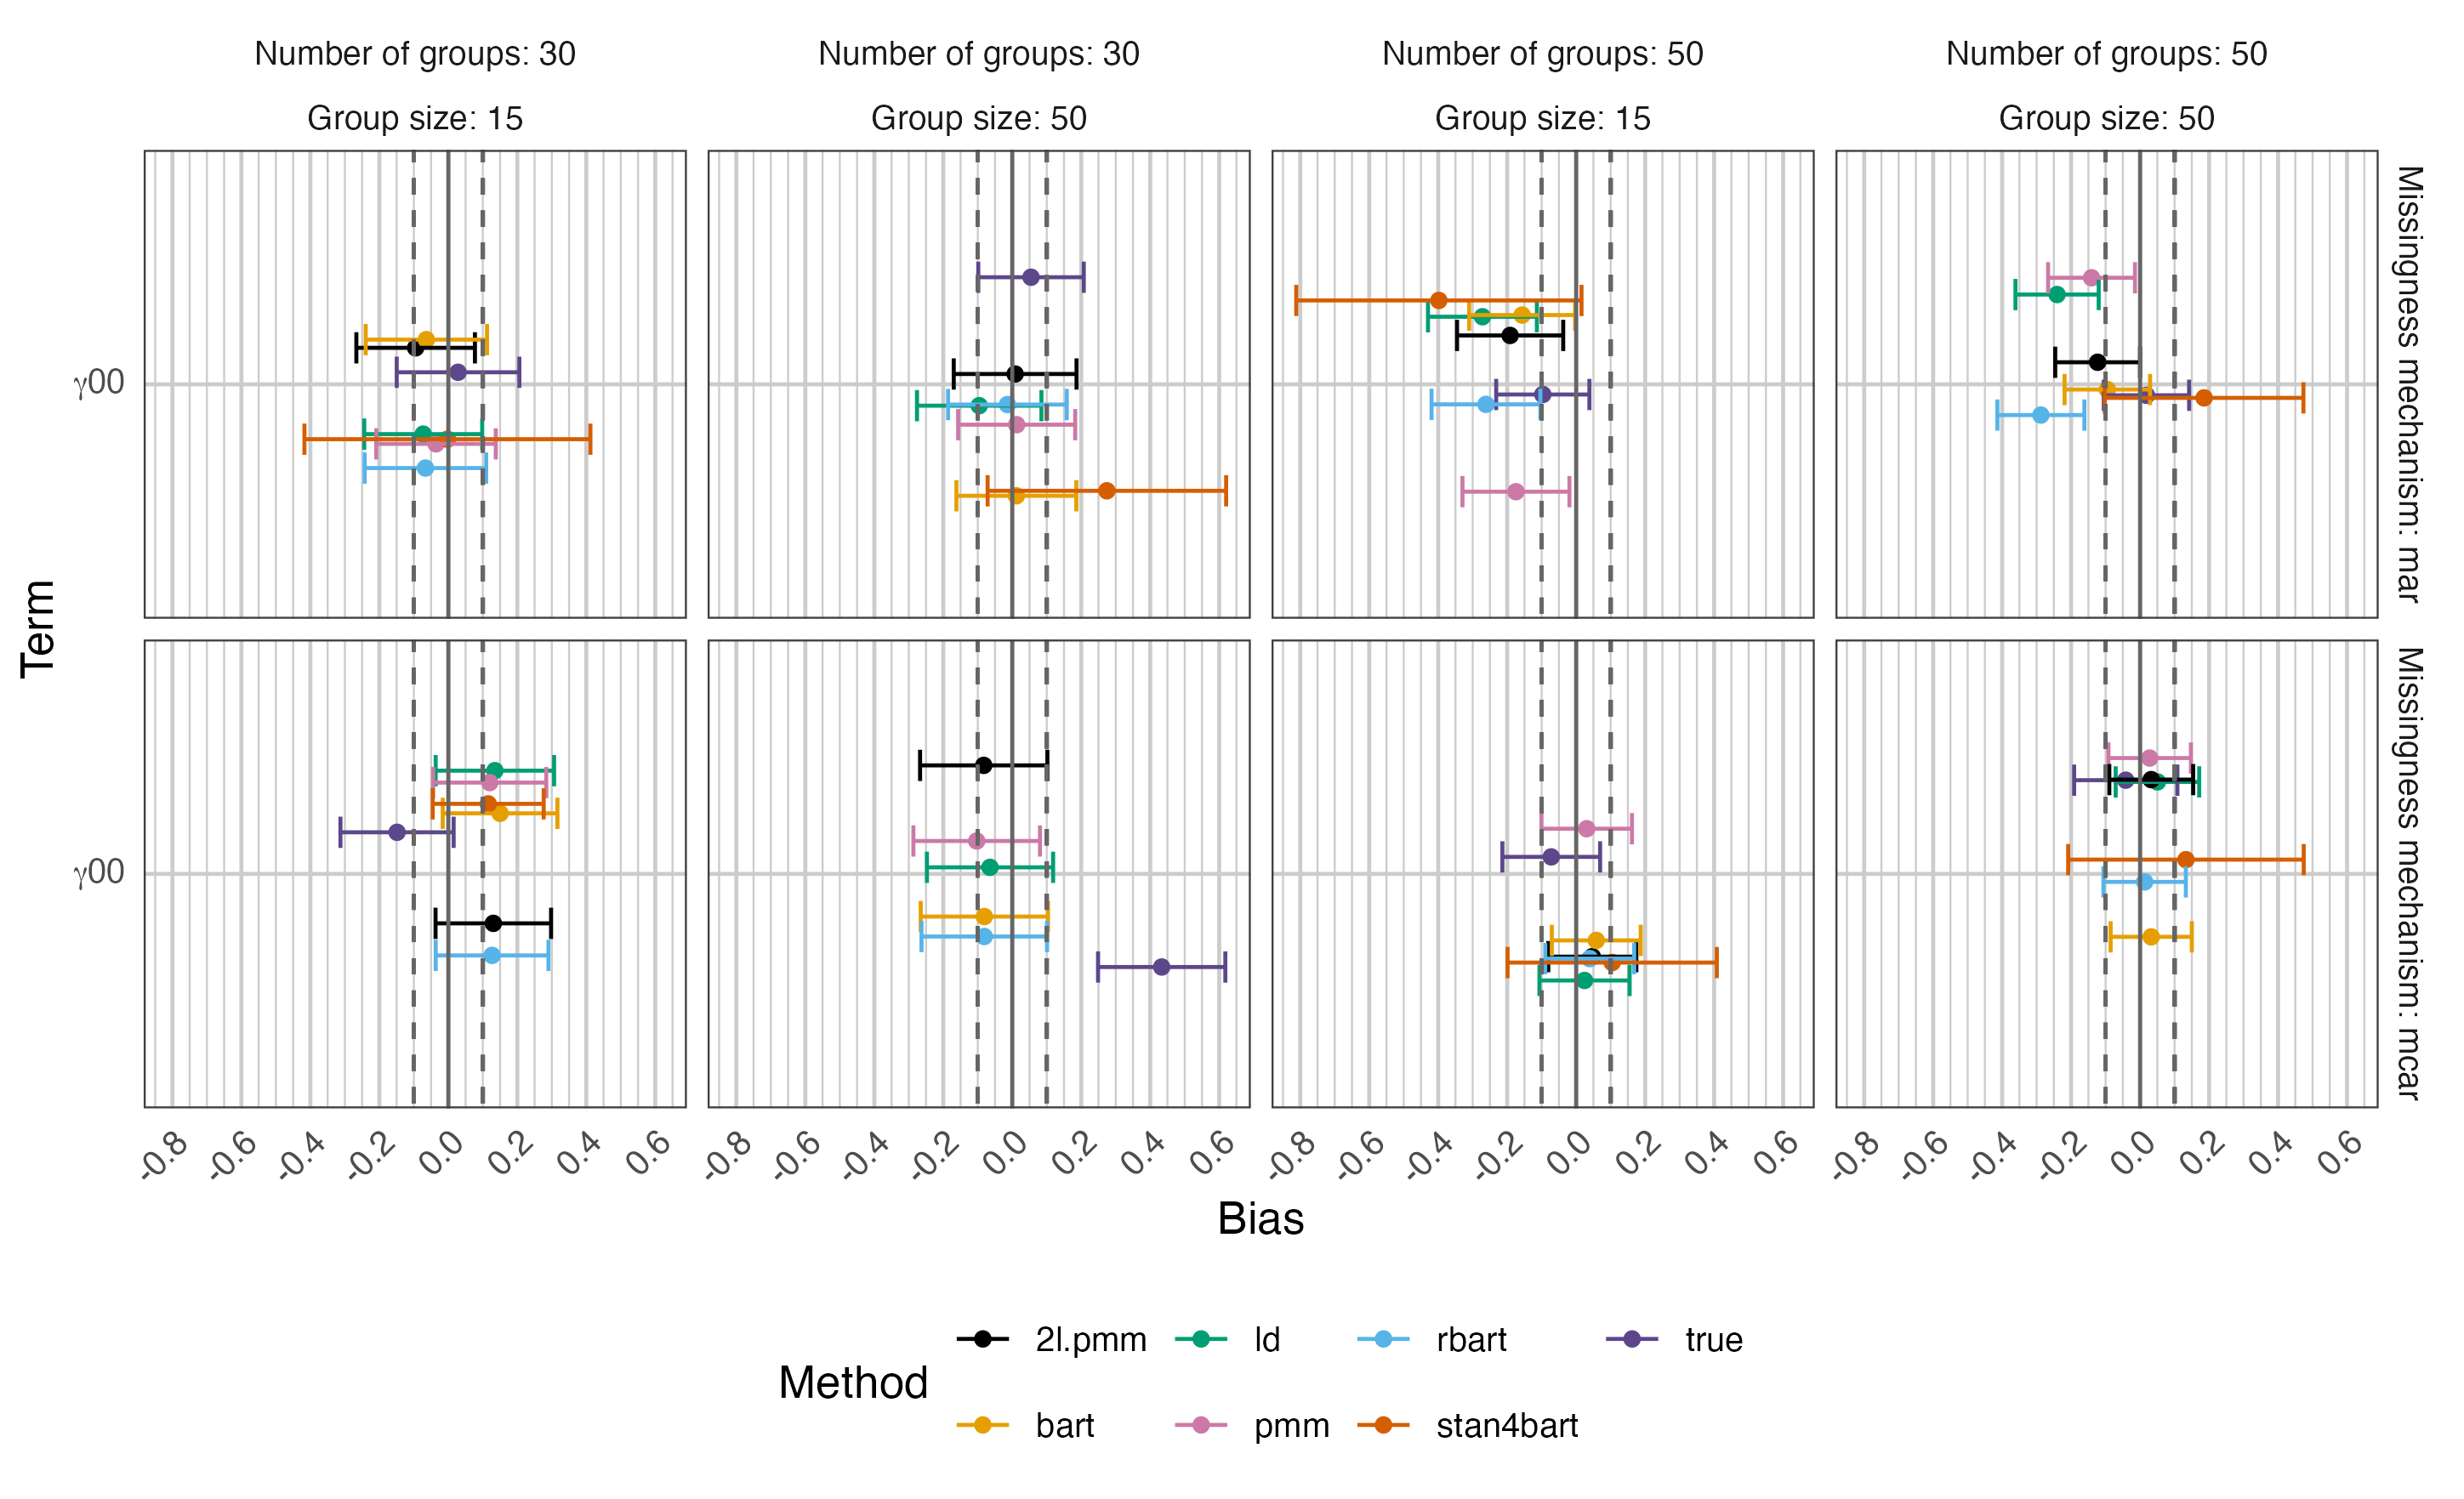
\includegraphics[width=1\textwidth]{biasintercept.png}
%     \caption{Absolute bias of the overall intercept of the linear mixed model with respective Monte Carlo SE for all simulated datasets over 100 simulations with ICC = .5. The dashed lines represent ±10\% relative bias.}
%     \label{fig:biasintercept}
%     % \caption*{\footnotesize{A note}}
% \end{figure}

Figure \ref{fig:biaslevel1} shows the absolute bias of the level-1 effects. When the sample size is smallest --- i.e. 30 groups of size 15 --- fluctuations in bias is more common for all methods when the data is MAR or MCAR. 2l.PMM, PMM, and BART seem to perform best out of all imputation methods for both missingness mechanisms, especially with a larger total sample size. Stan4bart seems to overestimate some fixed effects, which increases with the total sample size and when the data is MAR. Overall, R-BART has the worst performance in terms of absolute bias, consistently underestimating some level-1 effects.

% \begin{figure}[H]
%     \centering 
%     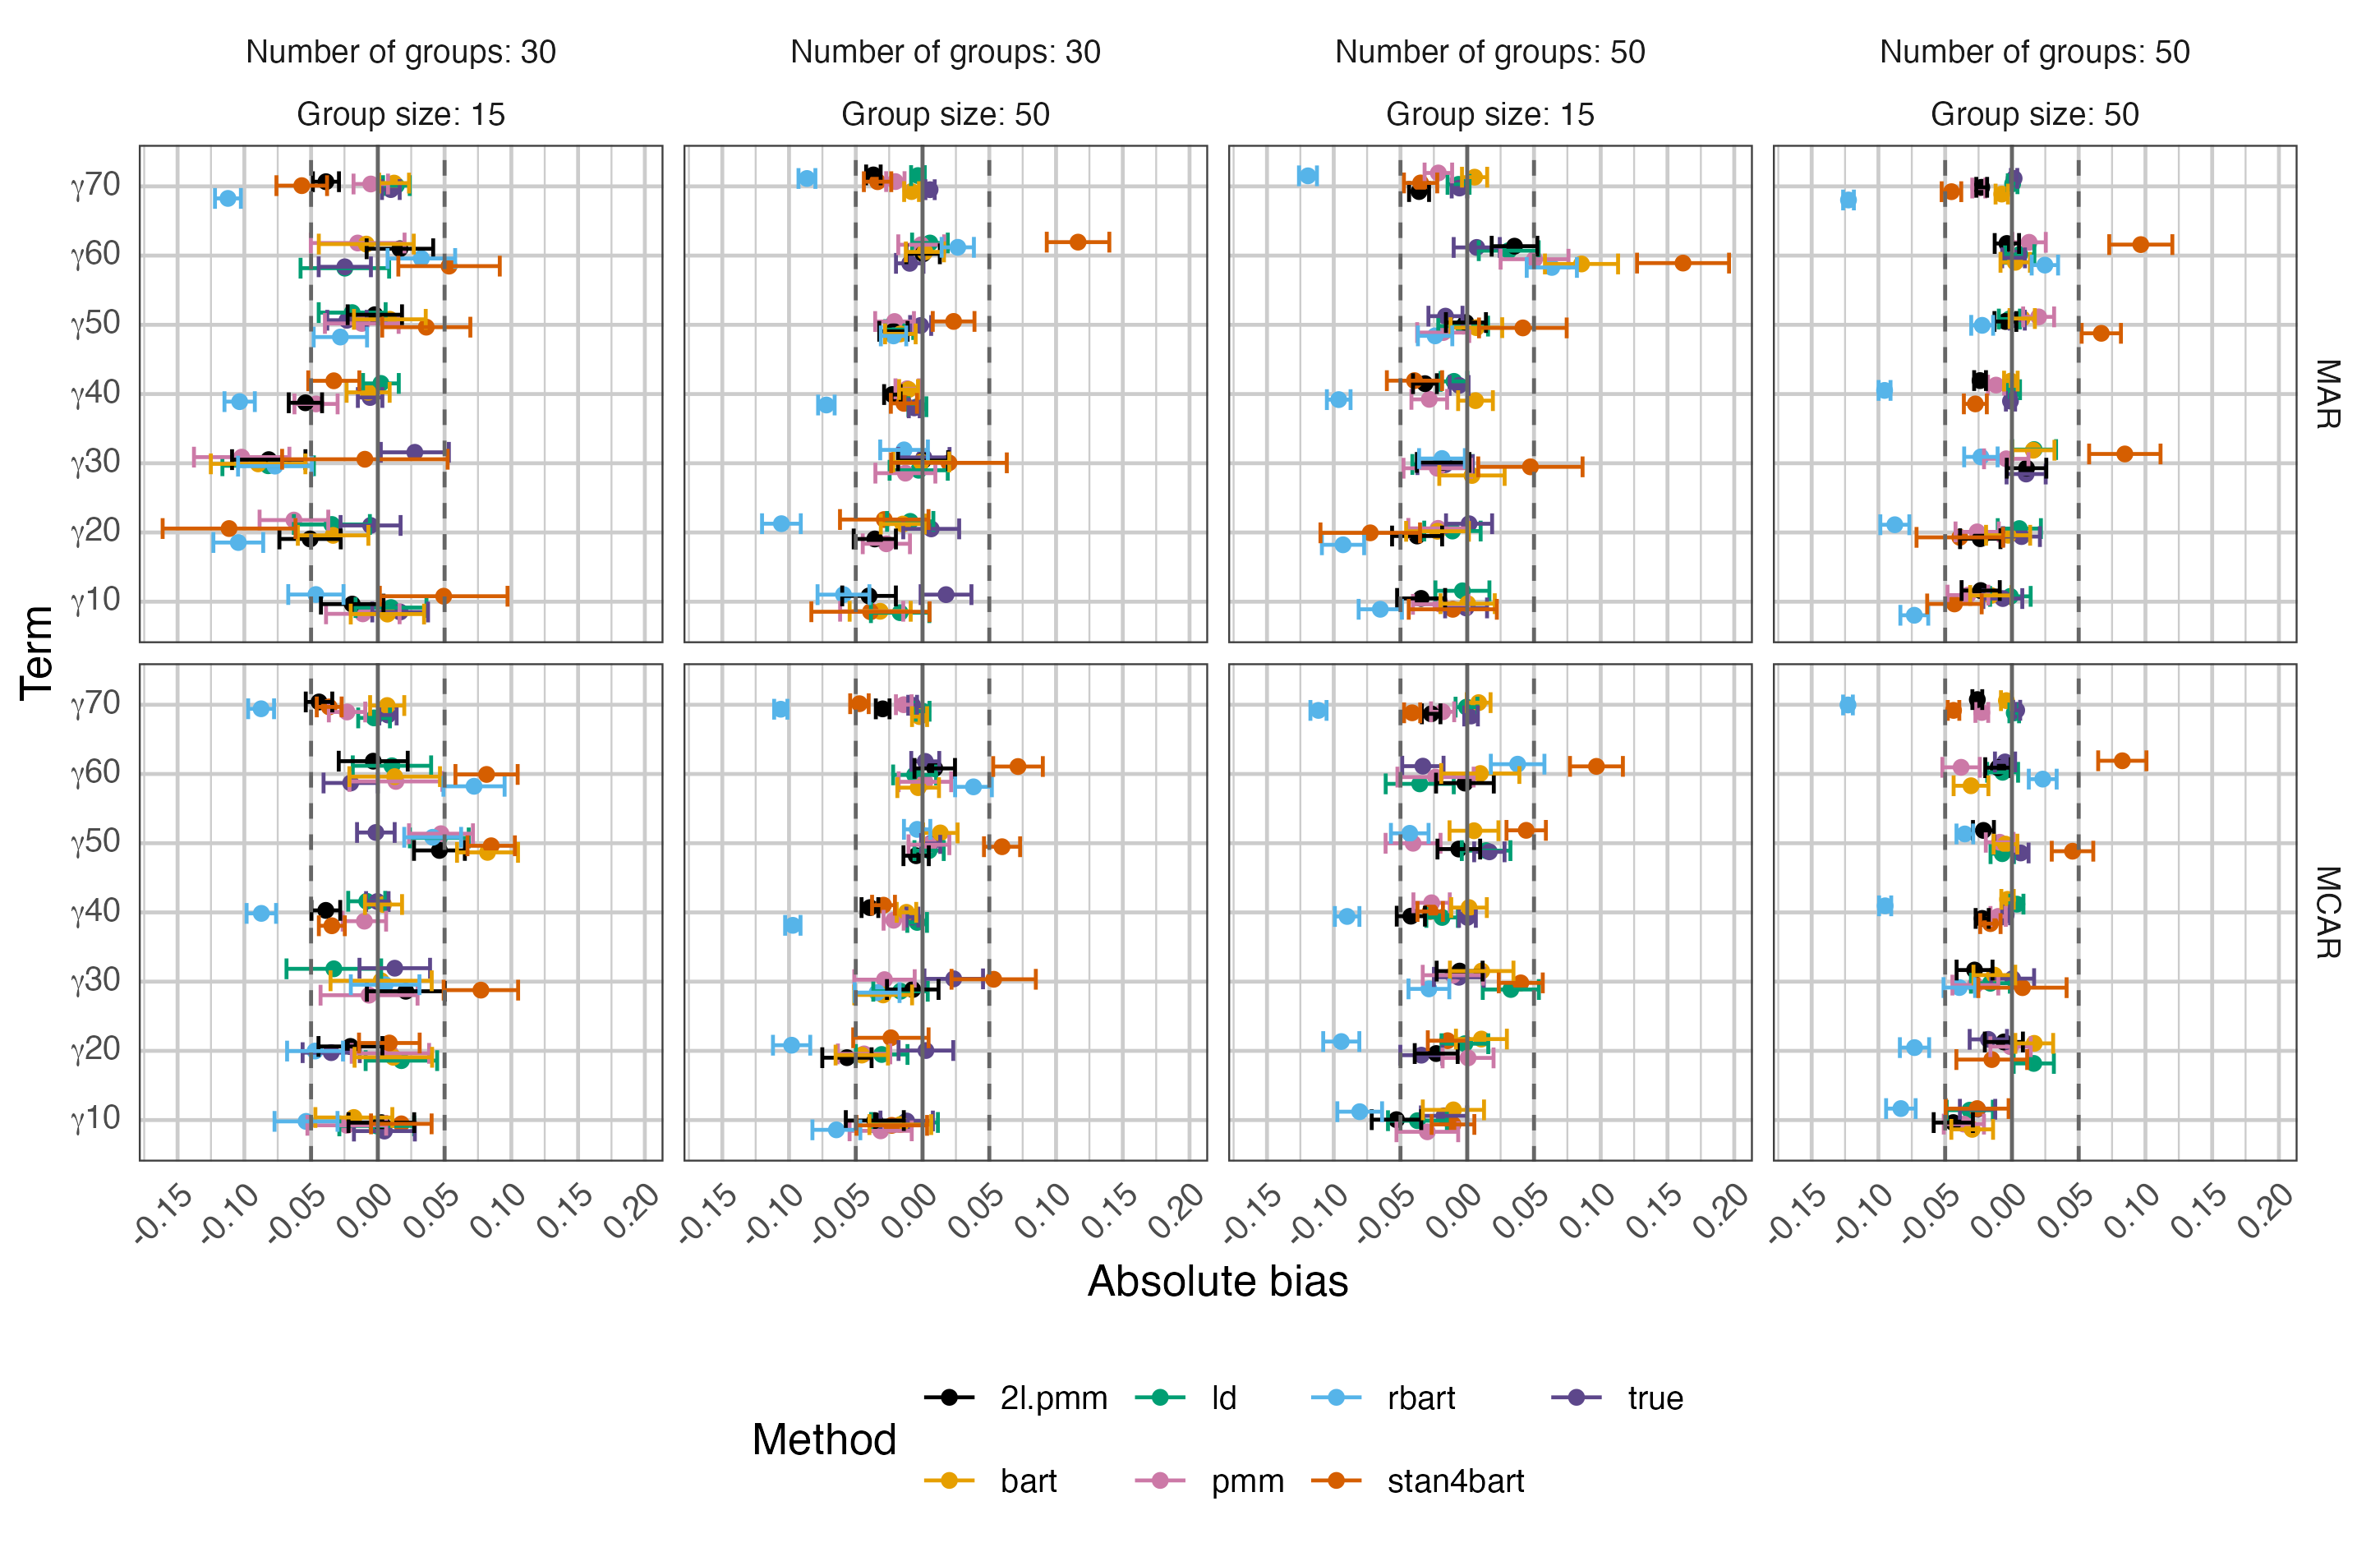
\includegraphics[width=1\textwidth]{biaslevel1.png}
%     \caption{Absolute bias of the level-1 effects of the linear mixed model with respective Monte Carlo SE for all simulated datasets over 100 simulations with ICC = .5.}
%     \label{fig:biaslevel1}
% \end{figure}

Considering the level-2 effects --- $\gamma_{01}$ and $\gamma_{02}$ --- from figure \ref{fig:biaslevel2}, stan4bart performs the worst out of all imputation methods in general: greatly underestimating the level-2 effects. 2l.PMM performs best out of all imputation methods, even though still over- or underestimating the level-2 effects at times and seemingly performing slightly worse under MCAR. PMM and R-BART consistently underestimate the level-2 effects for all conditions. BART performs slightly better, at times even mimicking the performance of 2l.PMM. 

% \begin{figure}[H]
%     \centering
%     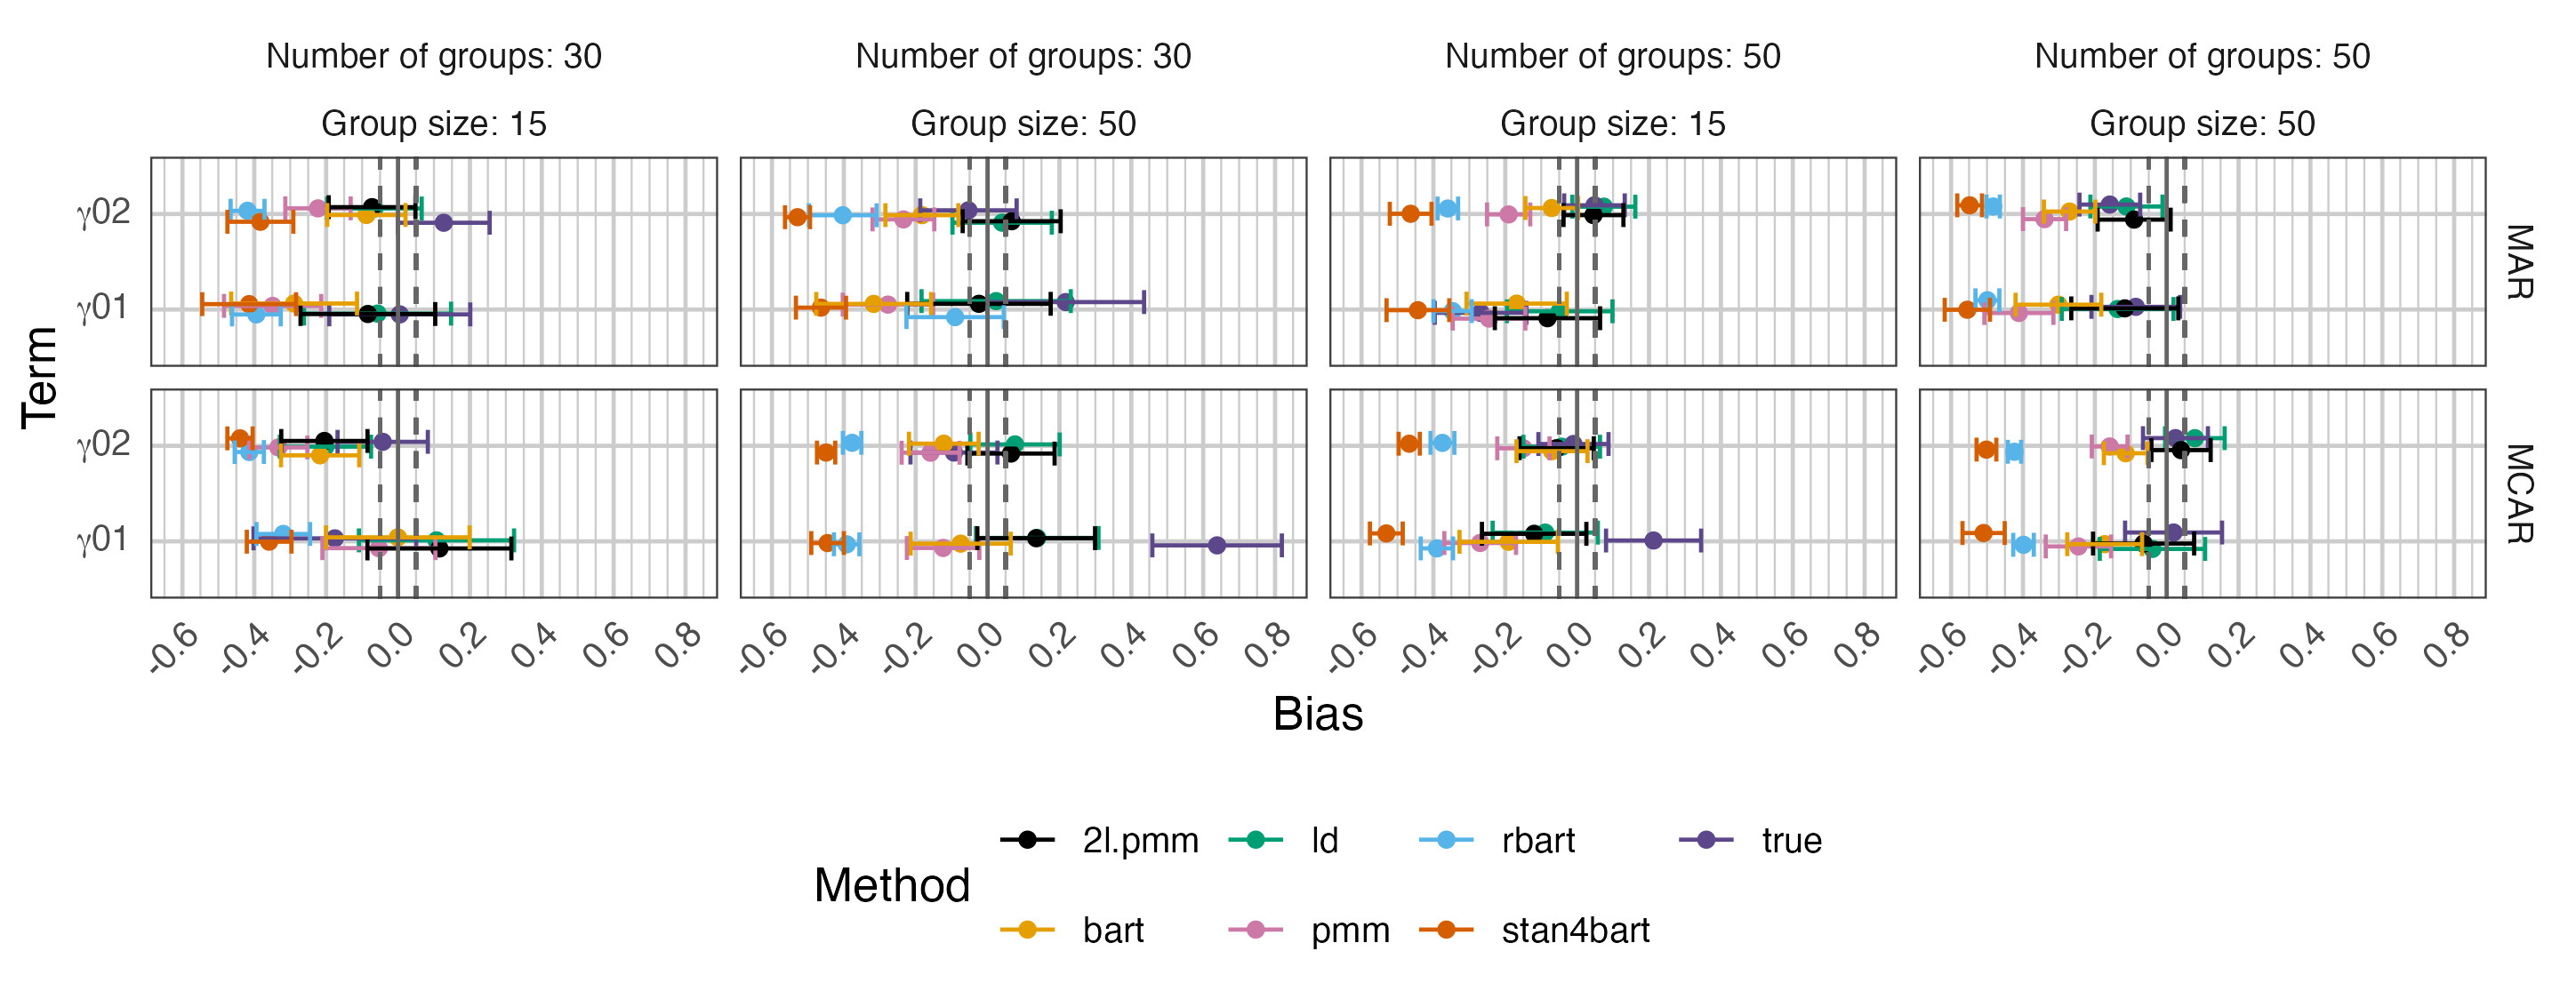
\includegraphics[width=1\textwidth]{biaslevel2.png}
%     \caption{Absolute bias of the level-2 effects of the linear mixed model with respective Monte Carlo SE for all simulated datasets over 100 simulations with ICC = .5.}
%     \label{fig:biaslevel2}
% \end{figure}

For the cross-level interactions --- $\gamma_{11}, \gamma_{21}$, and $\gamma_{32}$ ---, stan4bart has, again, the worst performance out of all methods. Figure \ref{fig:biascrosslevel} shows that stan4bart consistently underestimates the cross-level interactions for all conditions. For both MAR and MCAR, listwise deletion performs largely acceptable in terms of bias, often staying within the 10\% relative bias lines. 2l.PMM performs best out of all imputation methods, even though it still underestimates the cross-level interactions regularly and performs slightly better under MCAR than MAR. BART consistently outperforms PMM and R-BART, notwithstanding it still underestimates the cross-level interactions. Additionally, BART, R-BART and PMM seem to benefit from smaller groups. 

% \begin{figure}[H]
%     \centering
%     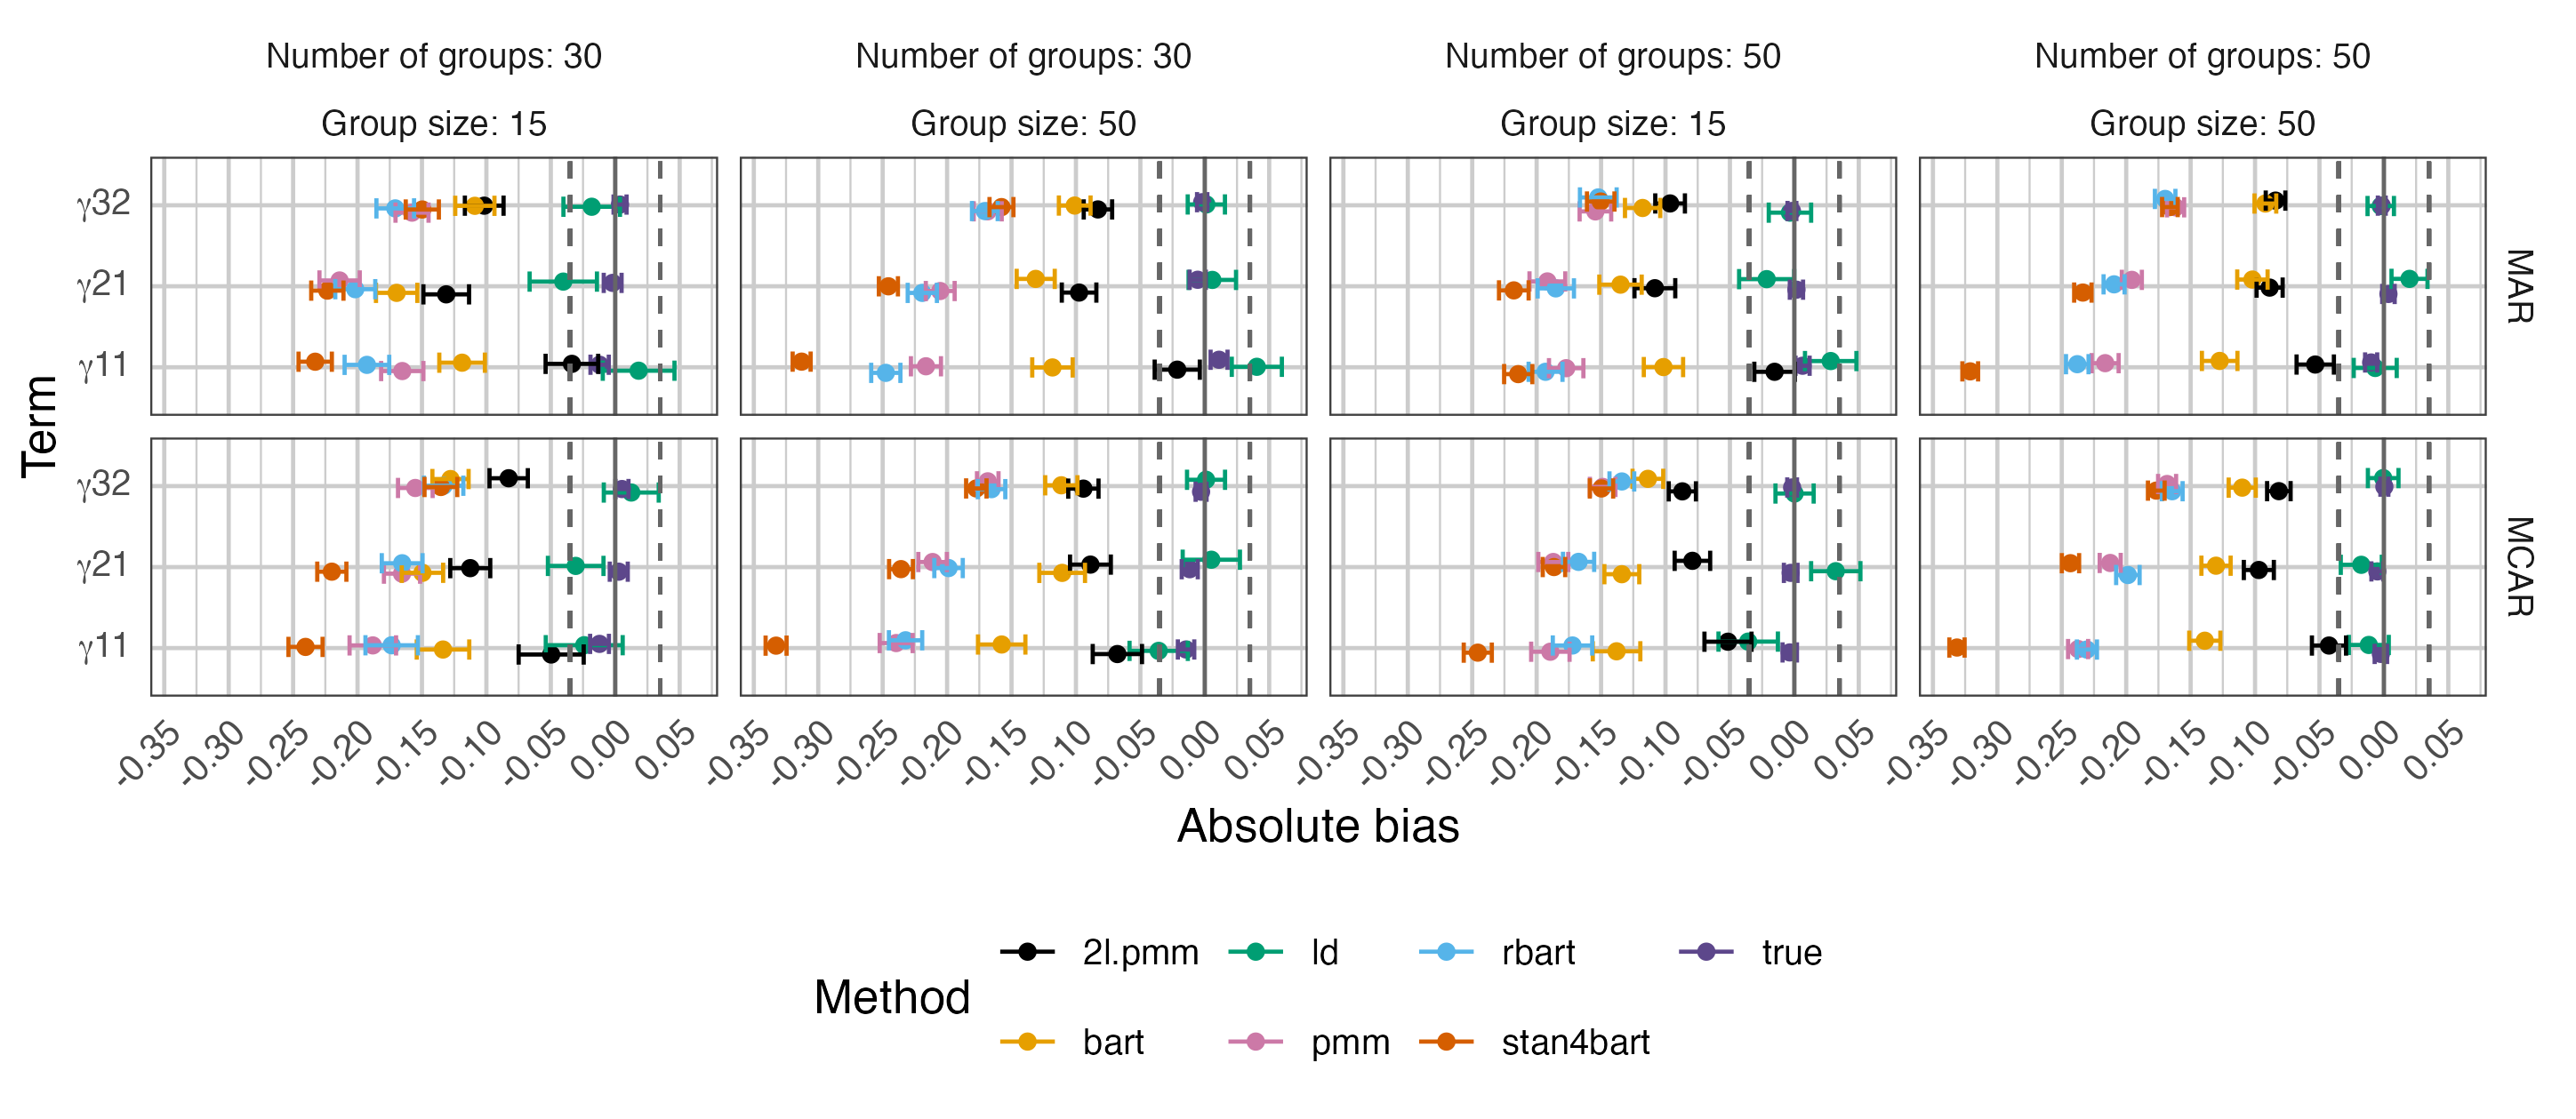
\includegraphics[width=1\textwidth]{biascrosslevel.png}
%     \caption{Absolute bias of the cross-level interactions of the linear mixed model with respective Monte Carlo SE for all simulated datasets over 100 simulations with ICC = .5.}
%     \label{fig:biascrosslevel}
% \end{figure}

The absolute bias for the random slopes in figure \ref{fig:biasrandom} show that stan4bart has the best overall performance out of all imputation methods. When the data is MAR, stan4bart provides acceptable biases when group sizes are 15 and underestimates the random slopes when group sizes are 50, which reduces when there are more groups. PMM, BART and R-BART have the worst performance: they consistently underestimate the random slopes for all factor conditions. While 2l.PMM does perform better than PMM, BART, and R-BART, it still underestimates the random slopes for almost all conditions. Listwise deletion performs largely acceptable in terms of bias, most of the time staying within the 10\% relative bias lines for both MAR and MCAR. Under MCAR, listwise deletion does tend to slightly overestimate the random slopes.

% \begin{figure}[H]
%     \centering
%     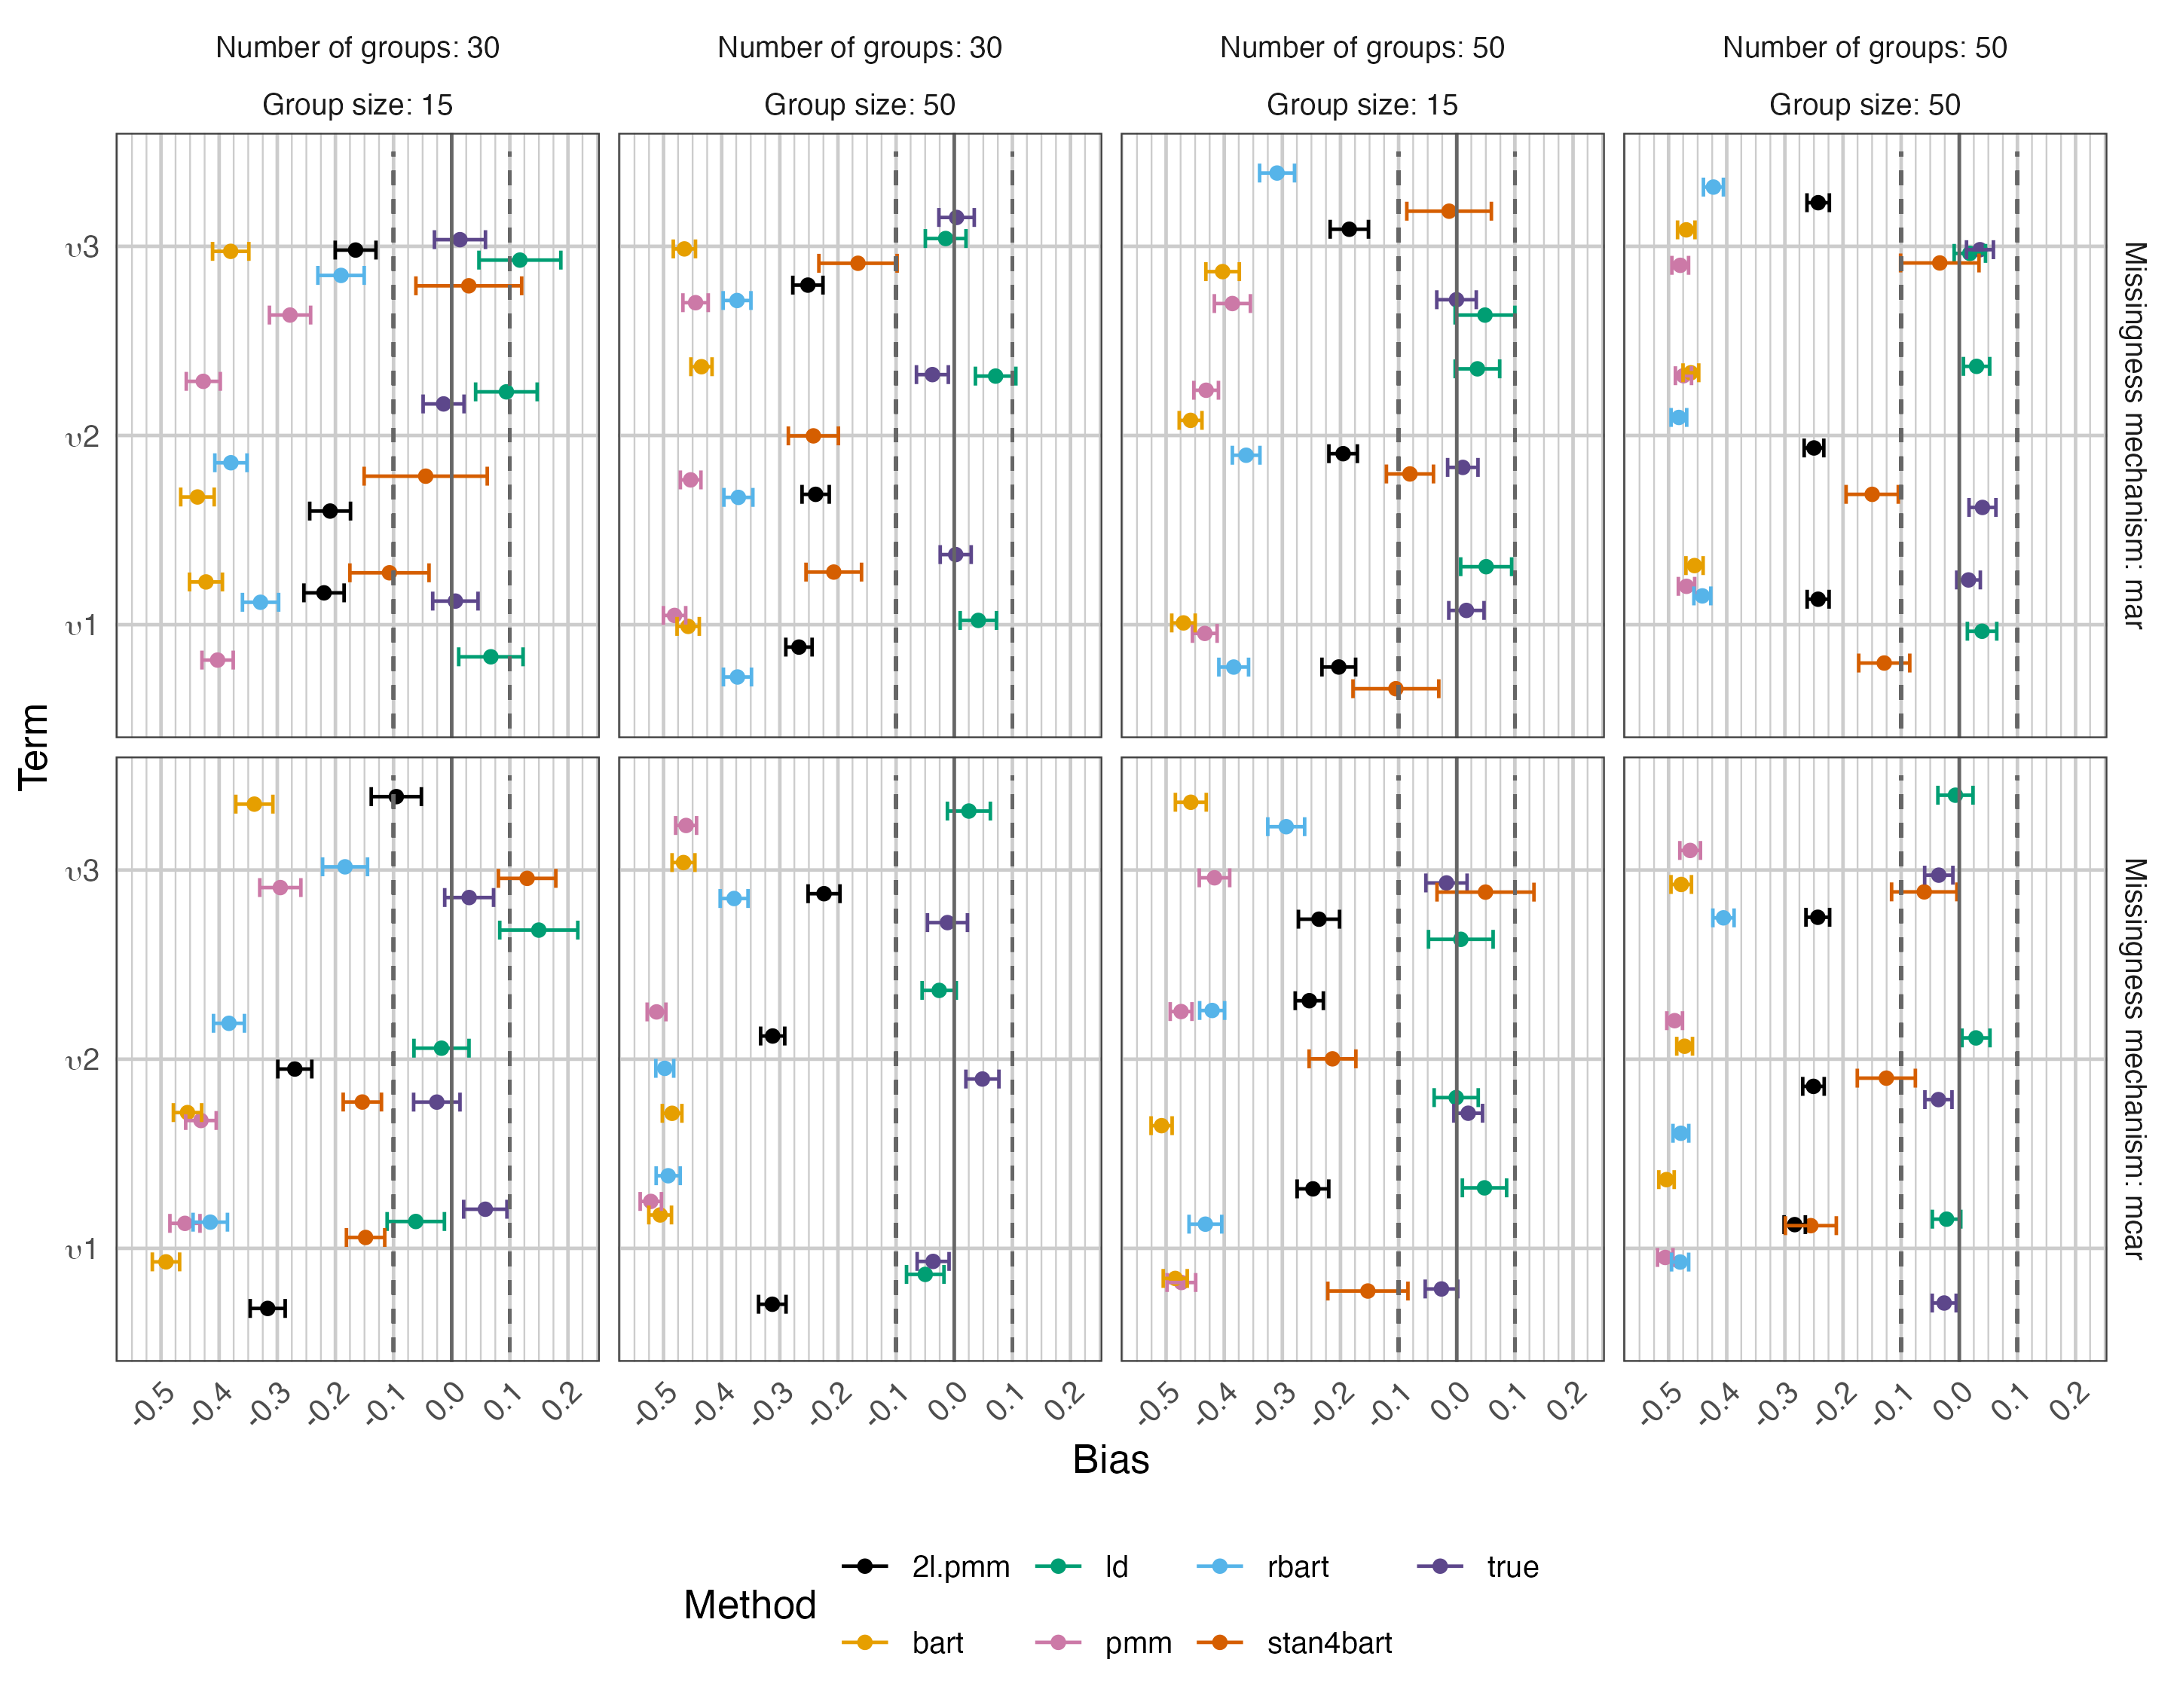
\includegraphics[width=1\textwidth]{biasrandom.png}
%     \caption{Absolute bias of the random slopes of the linear mixed model with respective Monte Carlo SE for all simulated datasets over 100 simulations with ICC = .5.}
%     \label{fig:biasrandom}
% \end{figure}

Lastly, the absolute bias for the intercept and residual variance will be discussed. From figure \ref{fig:bias2} it can be seen that stan4bart and 2l.PMM have an acceptable bias for the intercept variance for almost all conditions. Stan4bart seems to slightly overestimate the intercept variance when the data is MAR compared to MCAR. Additionally, stan4bart improves in absolute bias when there are more groups in the dataset. 2l.PMM slightly underestimates the intercept variance to an acceptable extend --- not more than 10\% in terms of relative bias --- for all conditions. PMM, R-BART and BART routinely underestimate the intercept variance for all conditions. Listwise deletion shows a very minor bias, underestimating the intercept variance when the data is MAR. 

Looking at the residual variance, listwise deletion is the only method that is acceptably biased for all --- or any --- condition. All other imputation methods routinely overestimate the residual variance. Stan4bart has the best performance followed by 2l.PMM, BART, PMM, and R-BART, in that order. Overall, the bias seems to be markedly consistent across all conditions. Aside from, stan4bart which seems to increase in bias when the total sample size increases and 2l.PMM which seems to decrease in bias with more groups in de dataset. 

\begin{figure}[H]
    \centering
    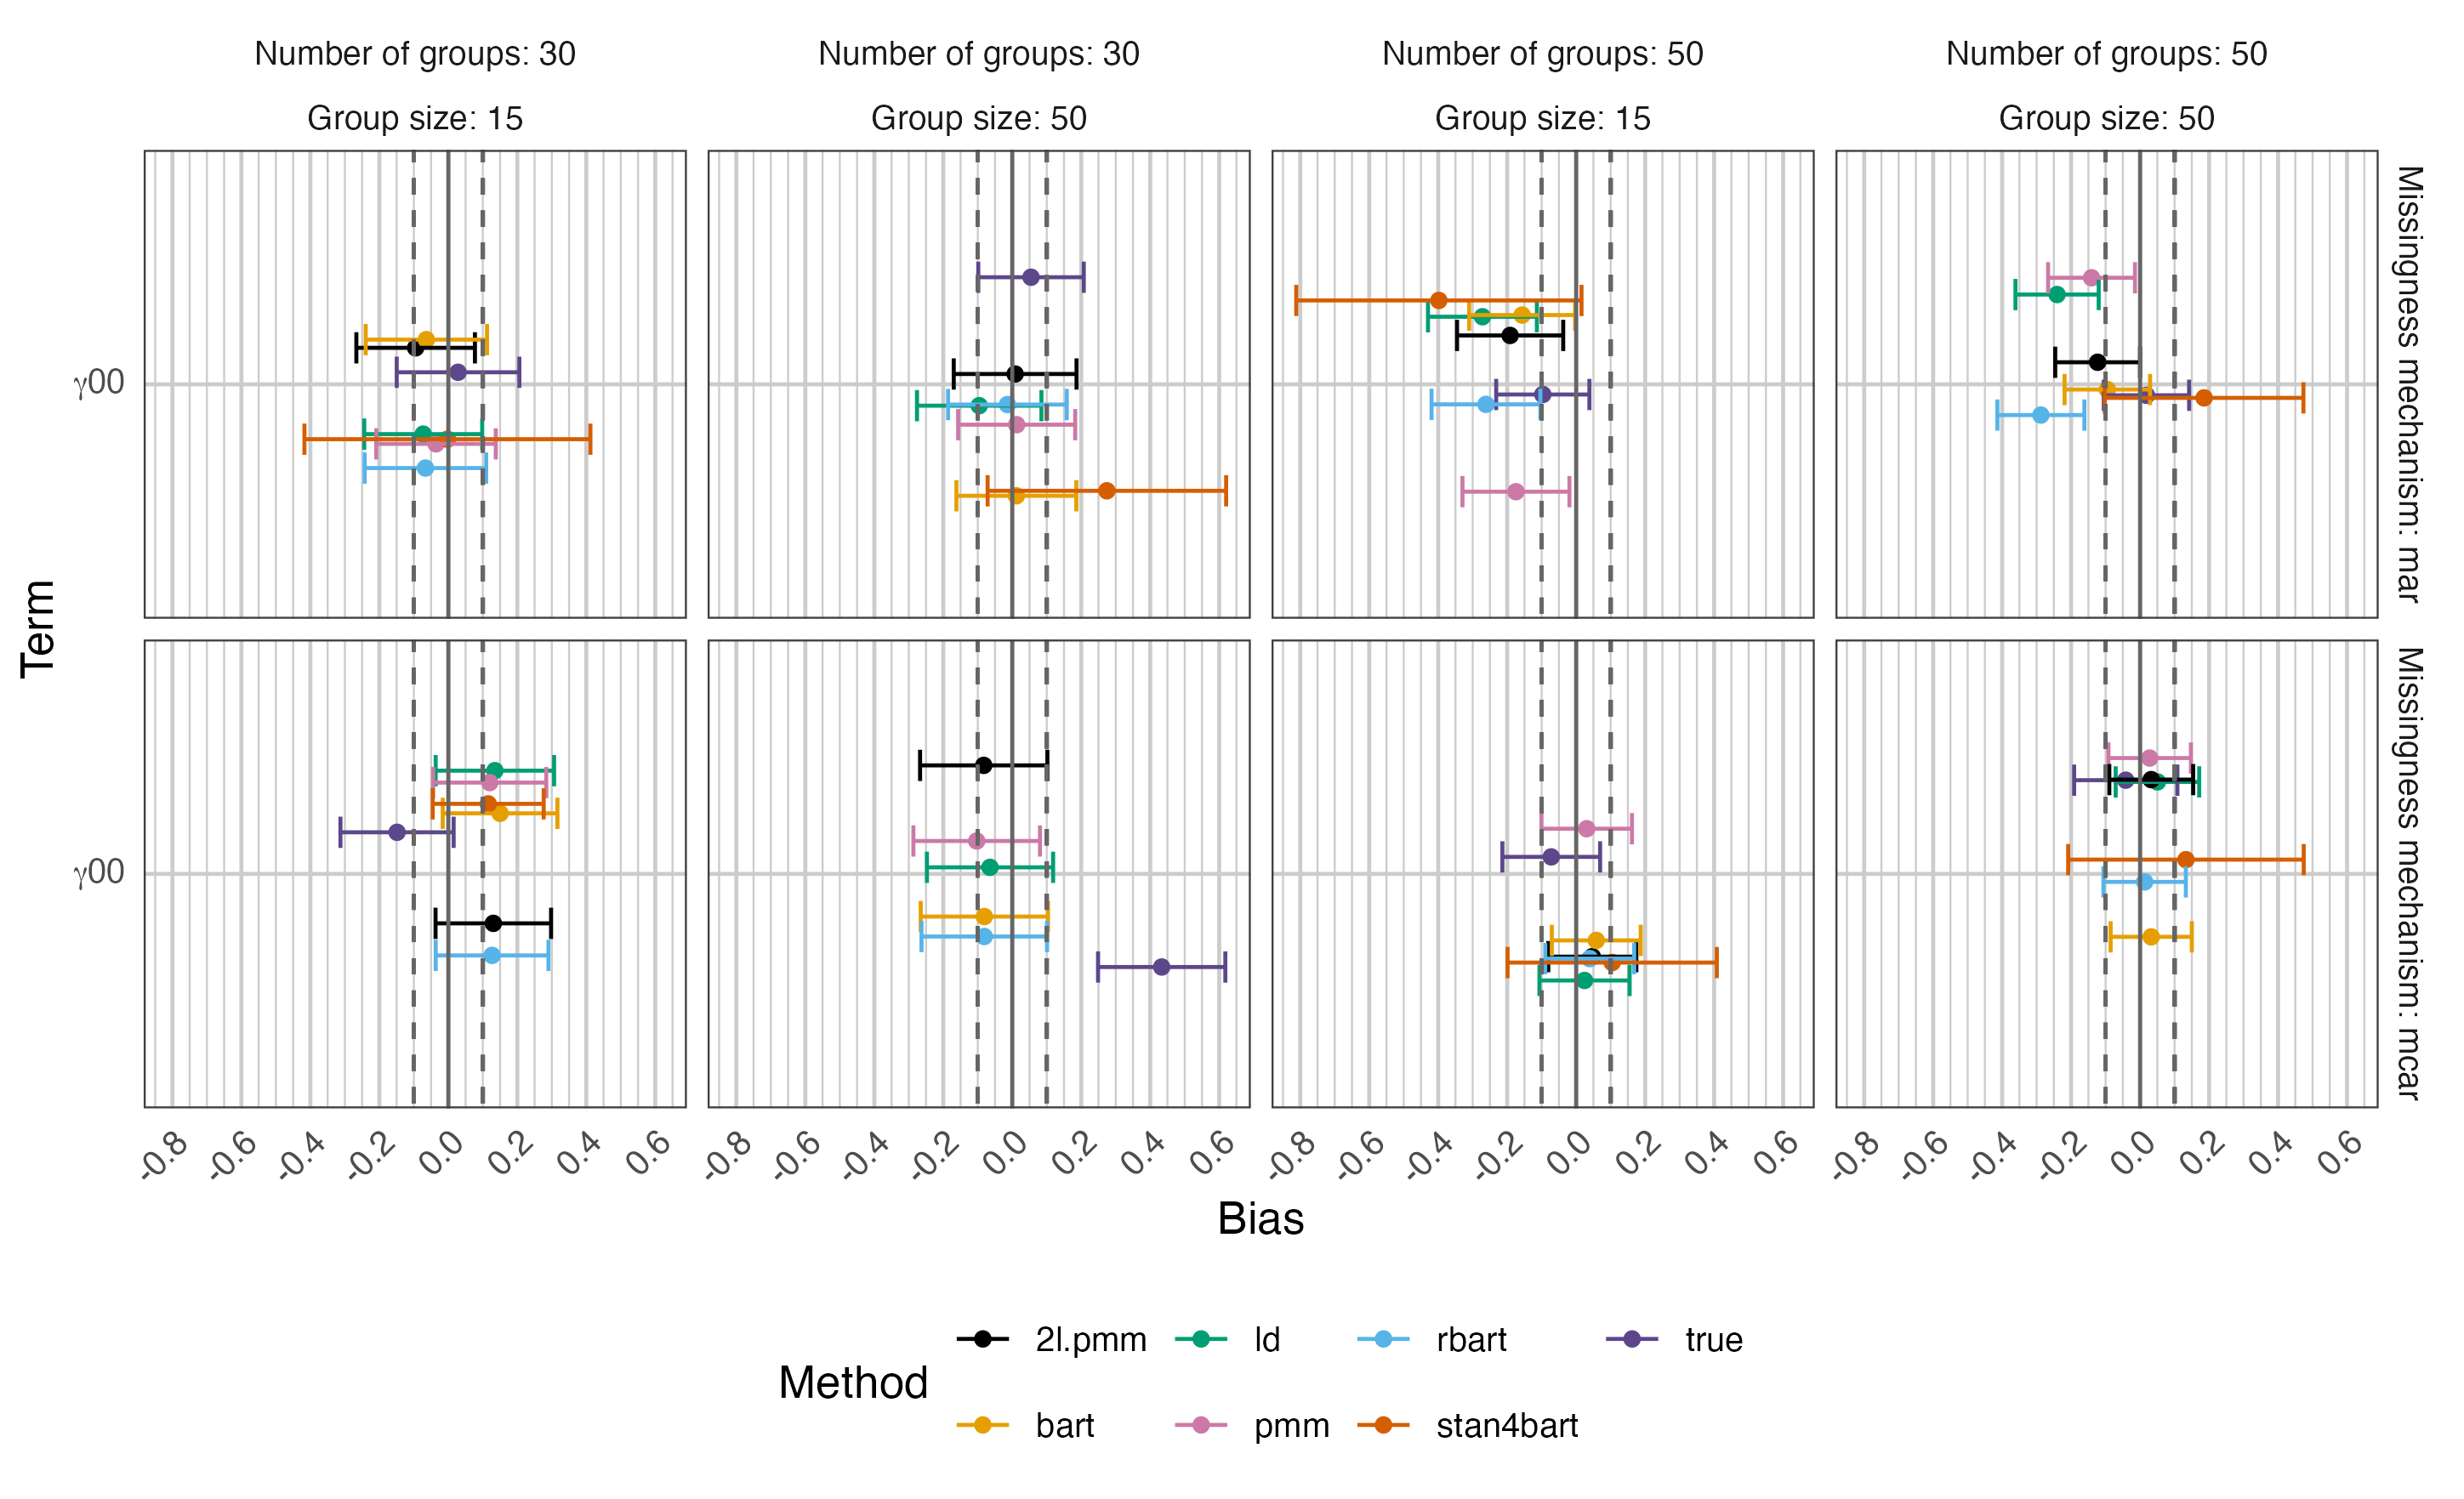
\includegraphics[width=1\textwidth]{biasintercept.png}
    \caption{Absolute bias of the overall intercept of the linear mixed model with respective Monte Carlo SE for all simulated datasets over 100 simulations with ICC = .5. The dashed lines represent ±10\% relative bias. Method stan4bart is based on a differing number of dataset simulations described in section \ref{sec:simulation}.}
    \label{fig:biasintercept}
    % \caption*{\footnotesize{A note}}
\end{figure}

\begin{figure}[H]
    \centering 
    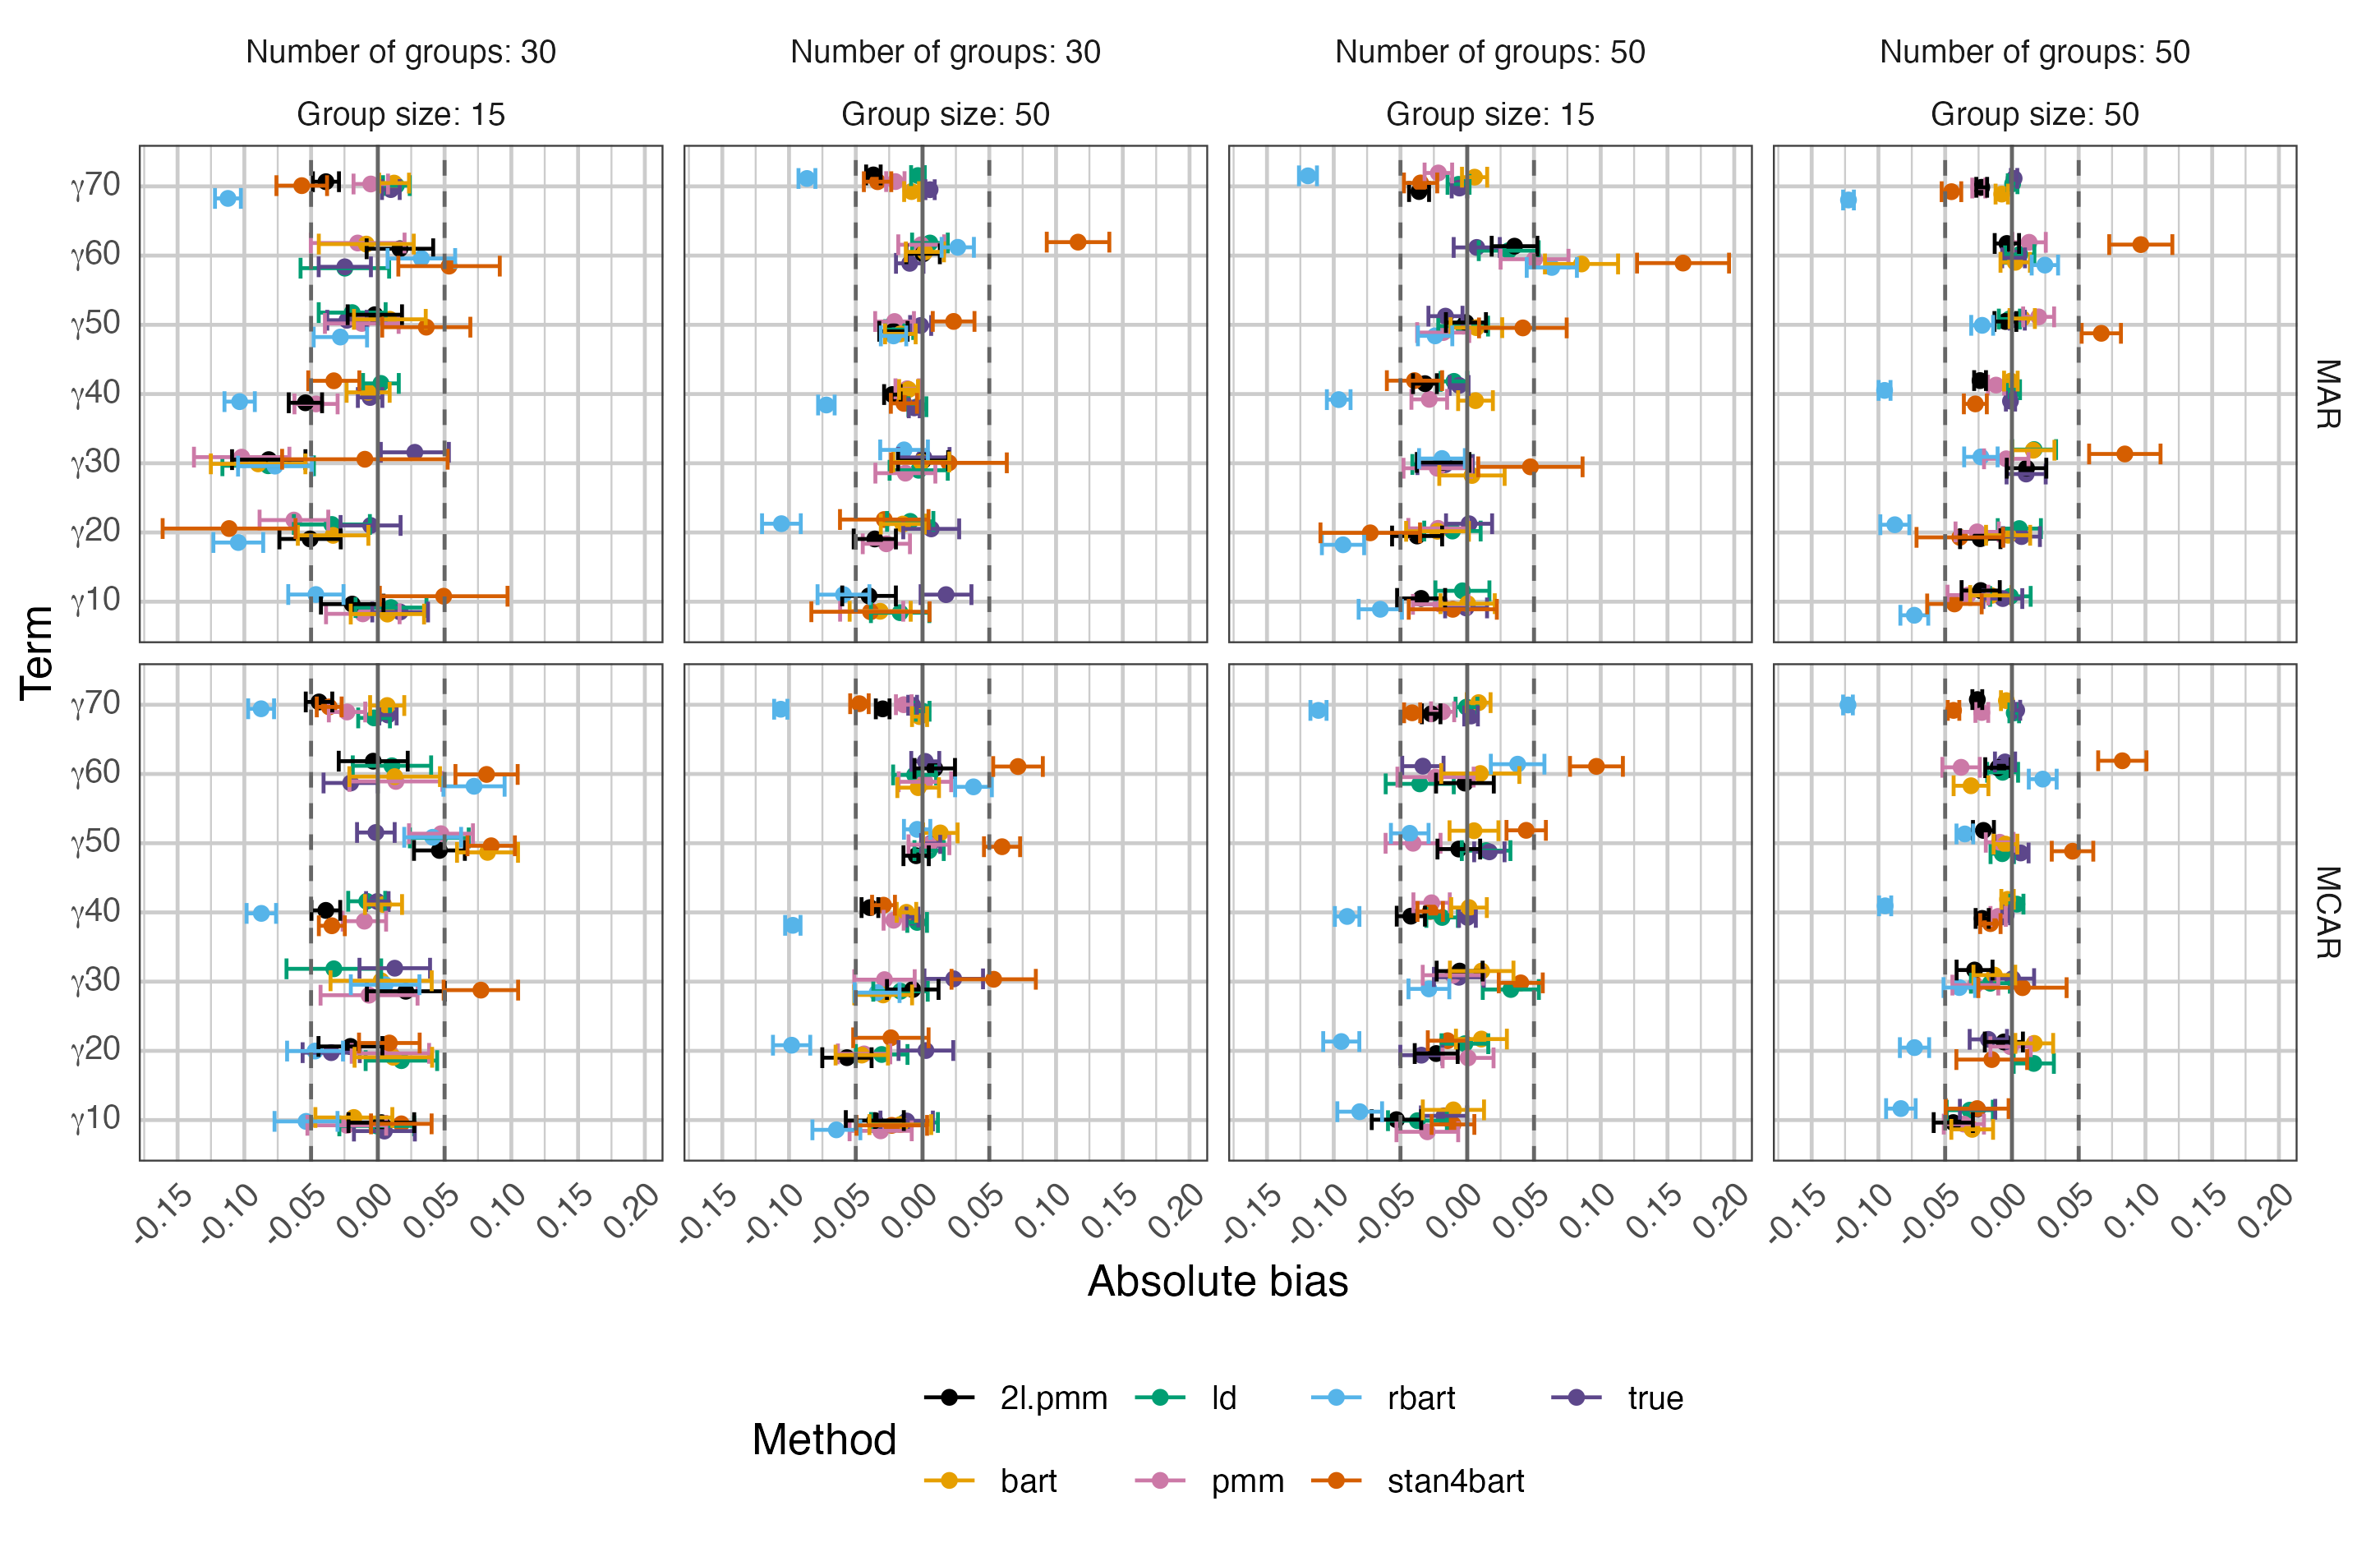
\includegraphics[width=1\textwidth]{biaslevel1.png}
    \caption{Absolute bias of the level-1 effects of the linear mixed model with respective Monte Carlo SE for all simulated datasets over 100 simulations with ICC = .5. The dashed lines represent ±10\% relative bias.}
    \label{fig:biaslevel1}
\end{figure}

\begin{figure}[H]
    \centering
    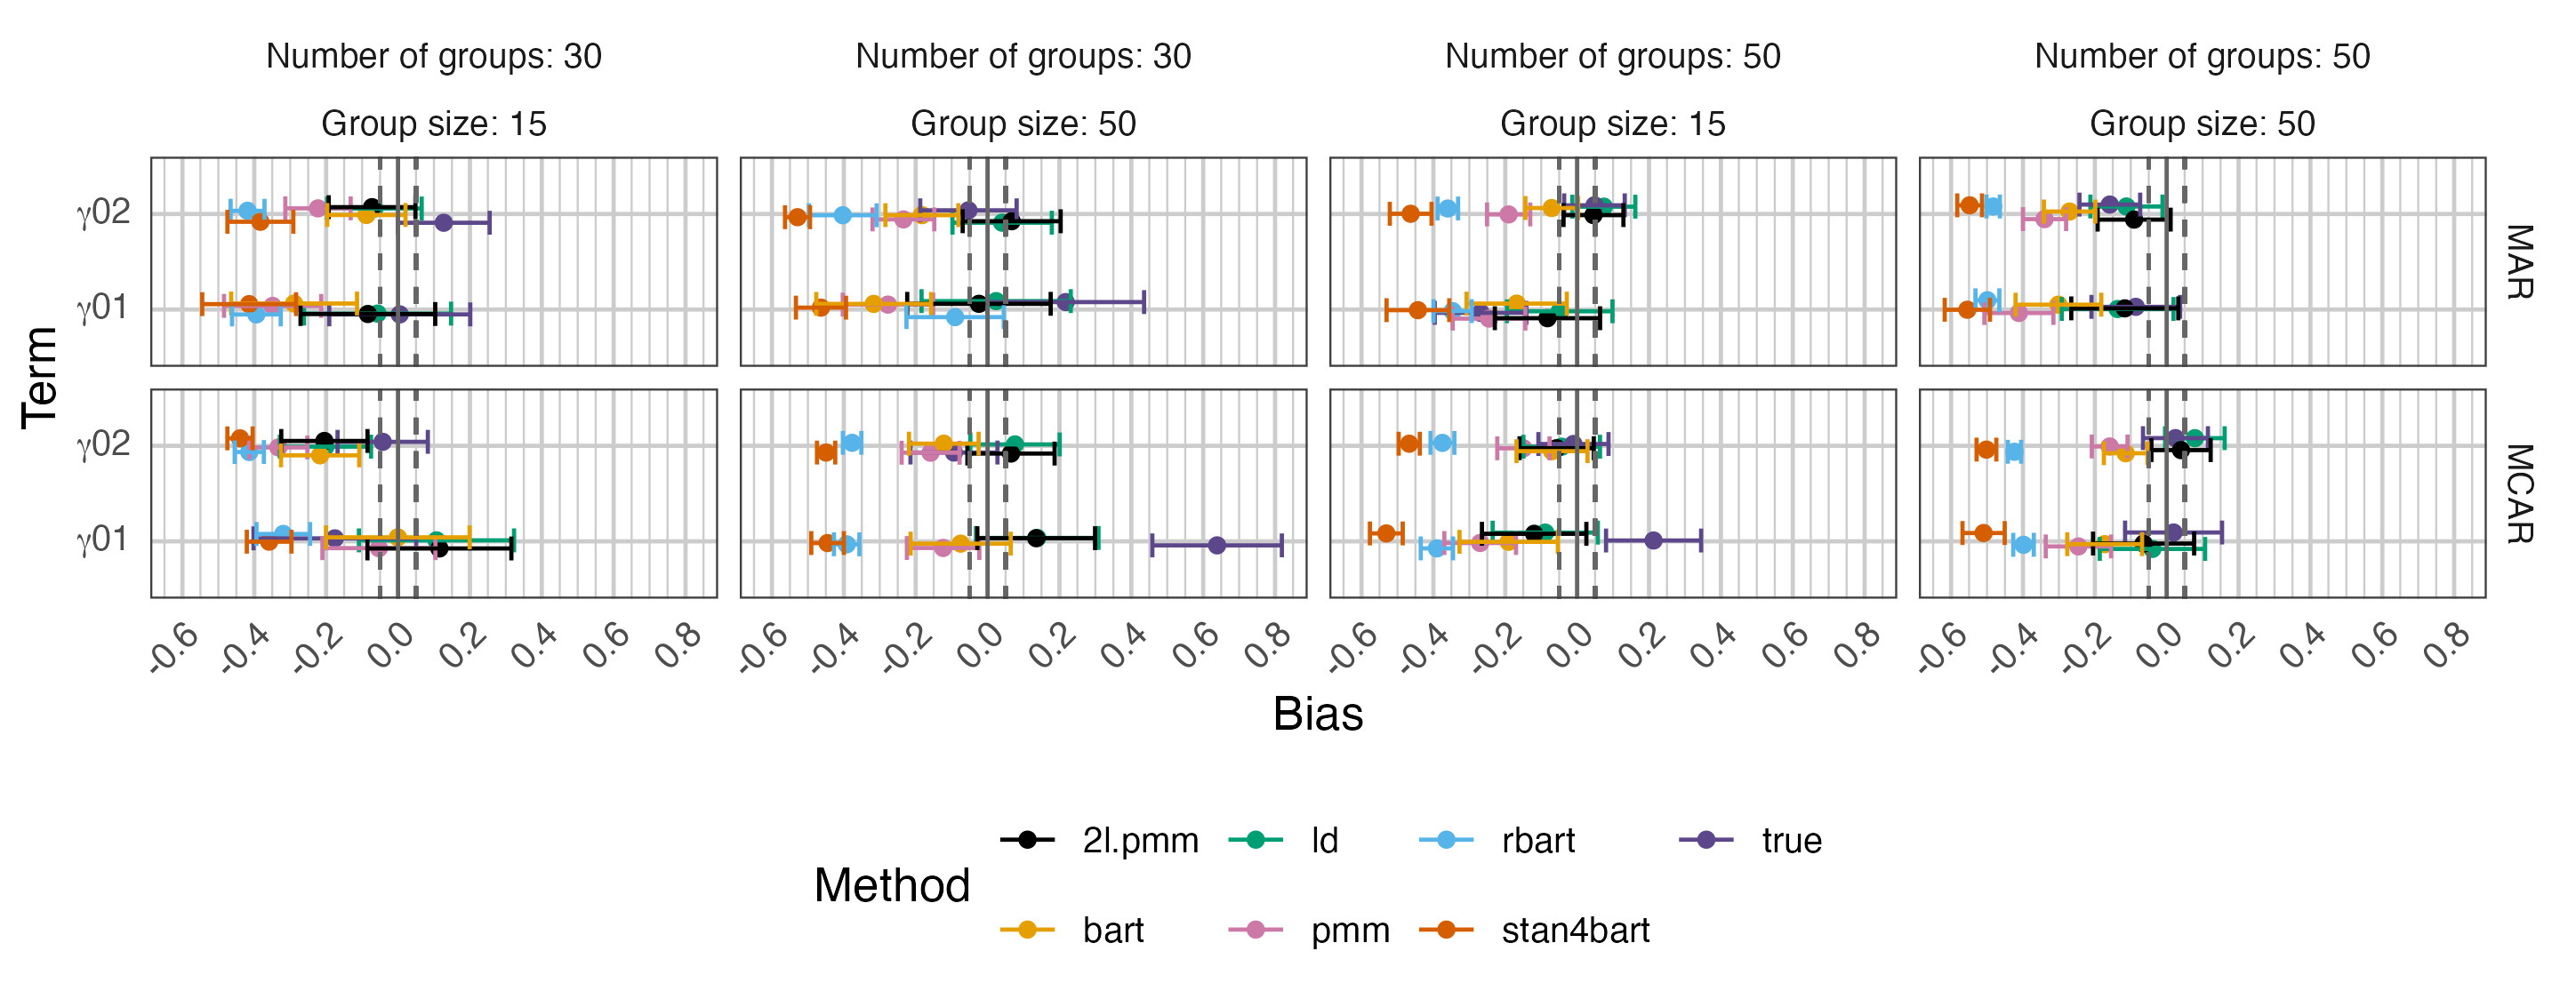
\includegraphics[width=1\textwidth]{biaslevel2.png}
    \caption{Absolute bias of the level-2 effects of the linear mixed model with respective Monte Carlo SE for all simulated datasets over 100 simulations with ICC = .5. The dashed lines represent ±10\% relative bias.}
    \label{fig:biaslevel2}
\end{figure}

\begin{figure}[H]
    \centering
    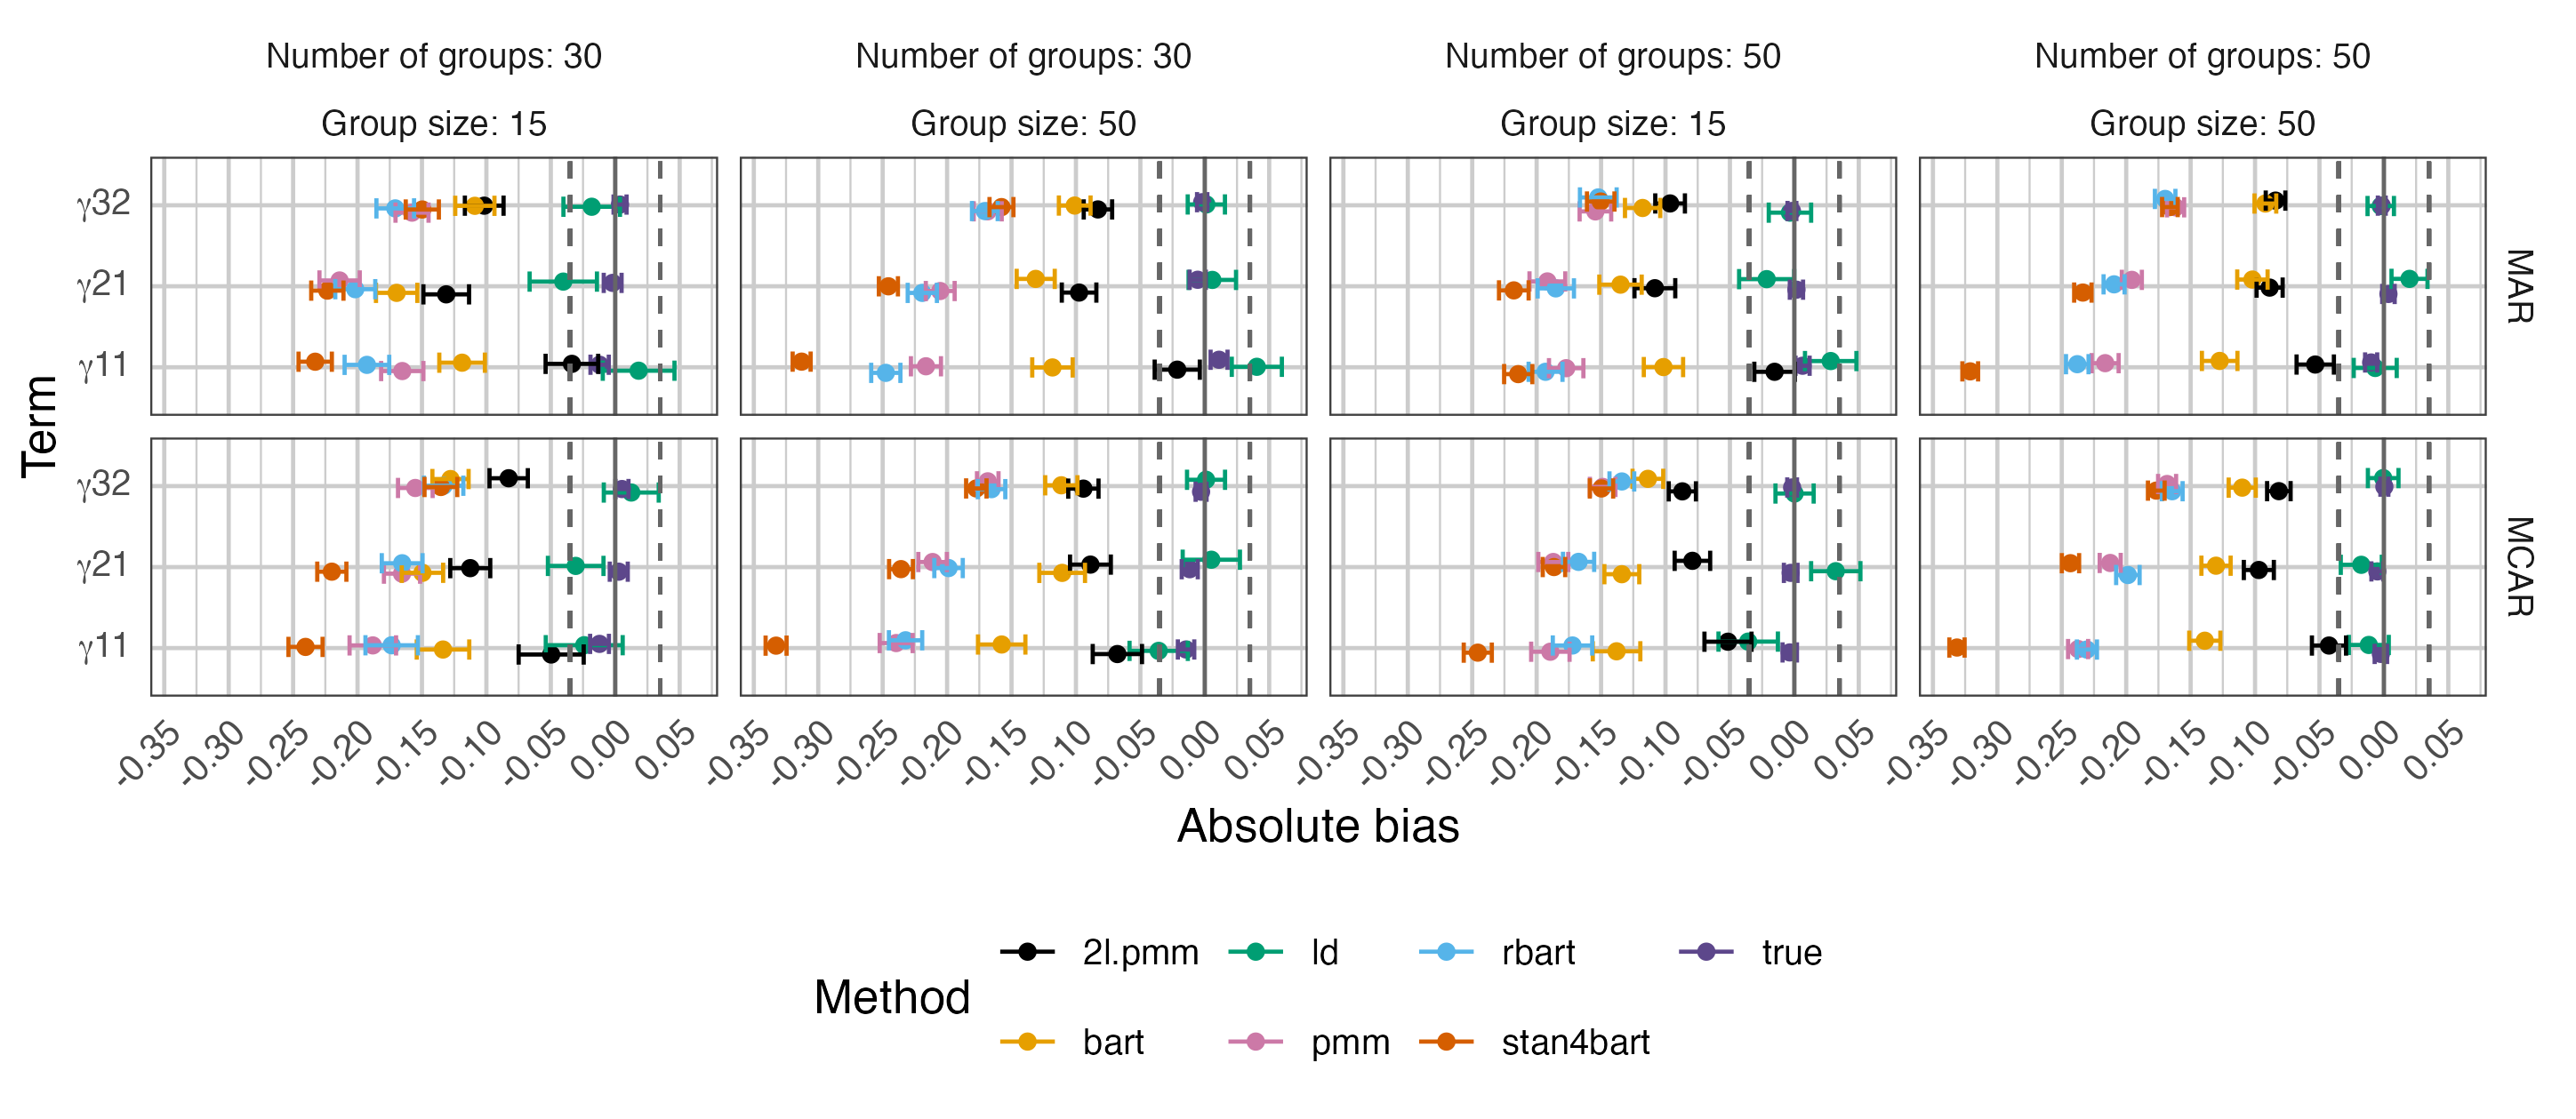
\includegraphics[width=1\textwidth]{biascrosslevel.png}
    \caption{Absolute bias of the cross-level interactions of the linear mixed model with respective Monte Carlo SE for all simulated datasets over 100 simulations with ICC = .5. The dashed lines represent ±10\% relative bias.}
    \label{fig:biascrosslevel}
\end{figure}

\begin{figure}[H]
    \centering
    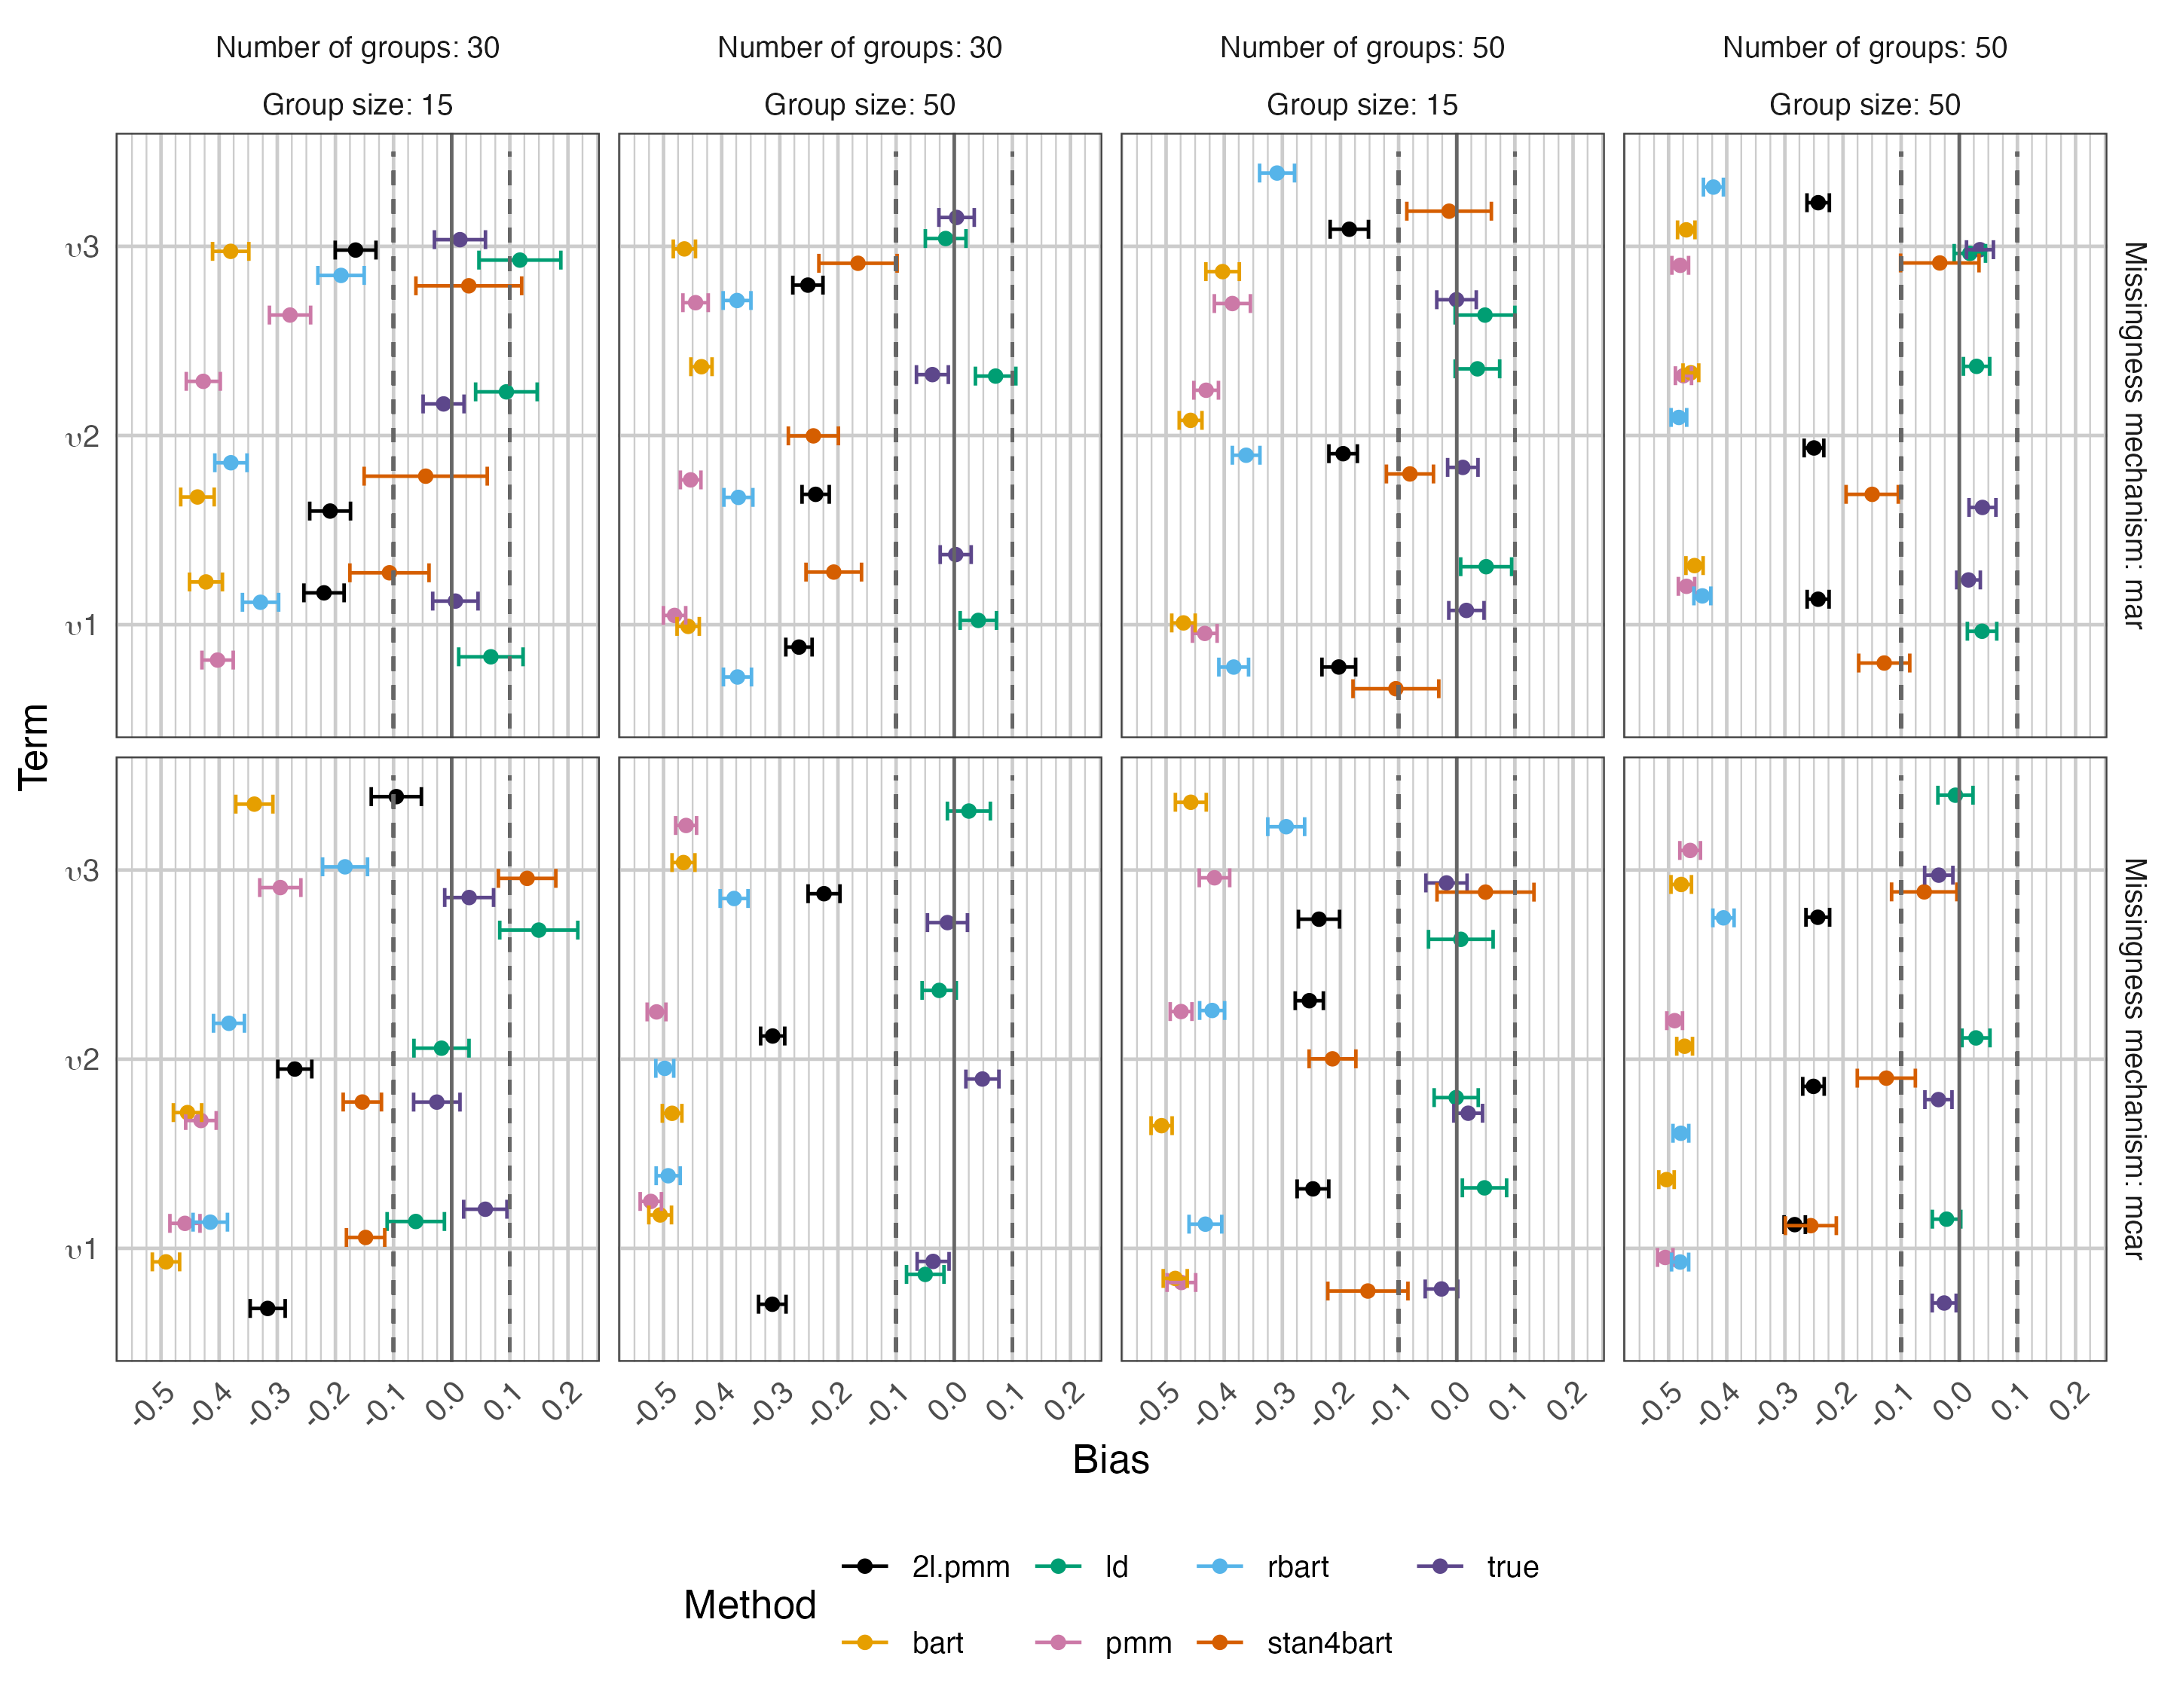
\includegraphics[width=1\textwidth]{biasrandom.png}
    \caption{Absolute bias of the random slopes of the linear mixed model with respective Monte Carlo SE for all simulated datasets over 100 simulations with ICC = .5. The dashed lines represent ±10\% relative bias.}
    \label{fig:biasrandom}
\end{figure}

\begin{figure}[H]
    \centering
    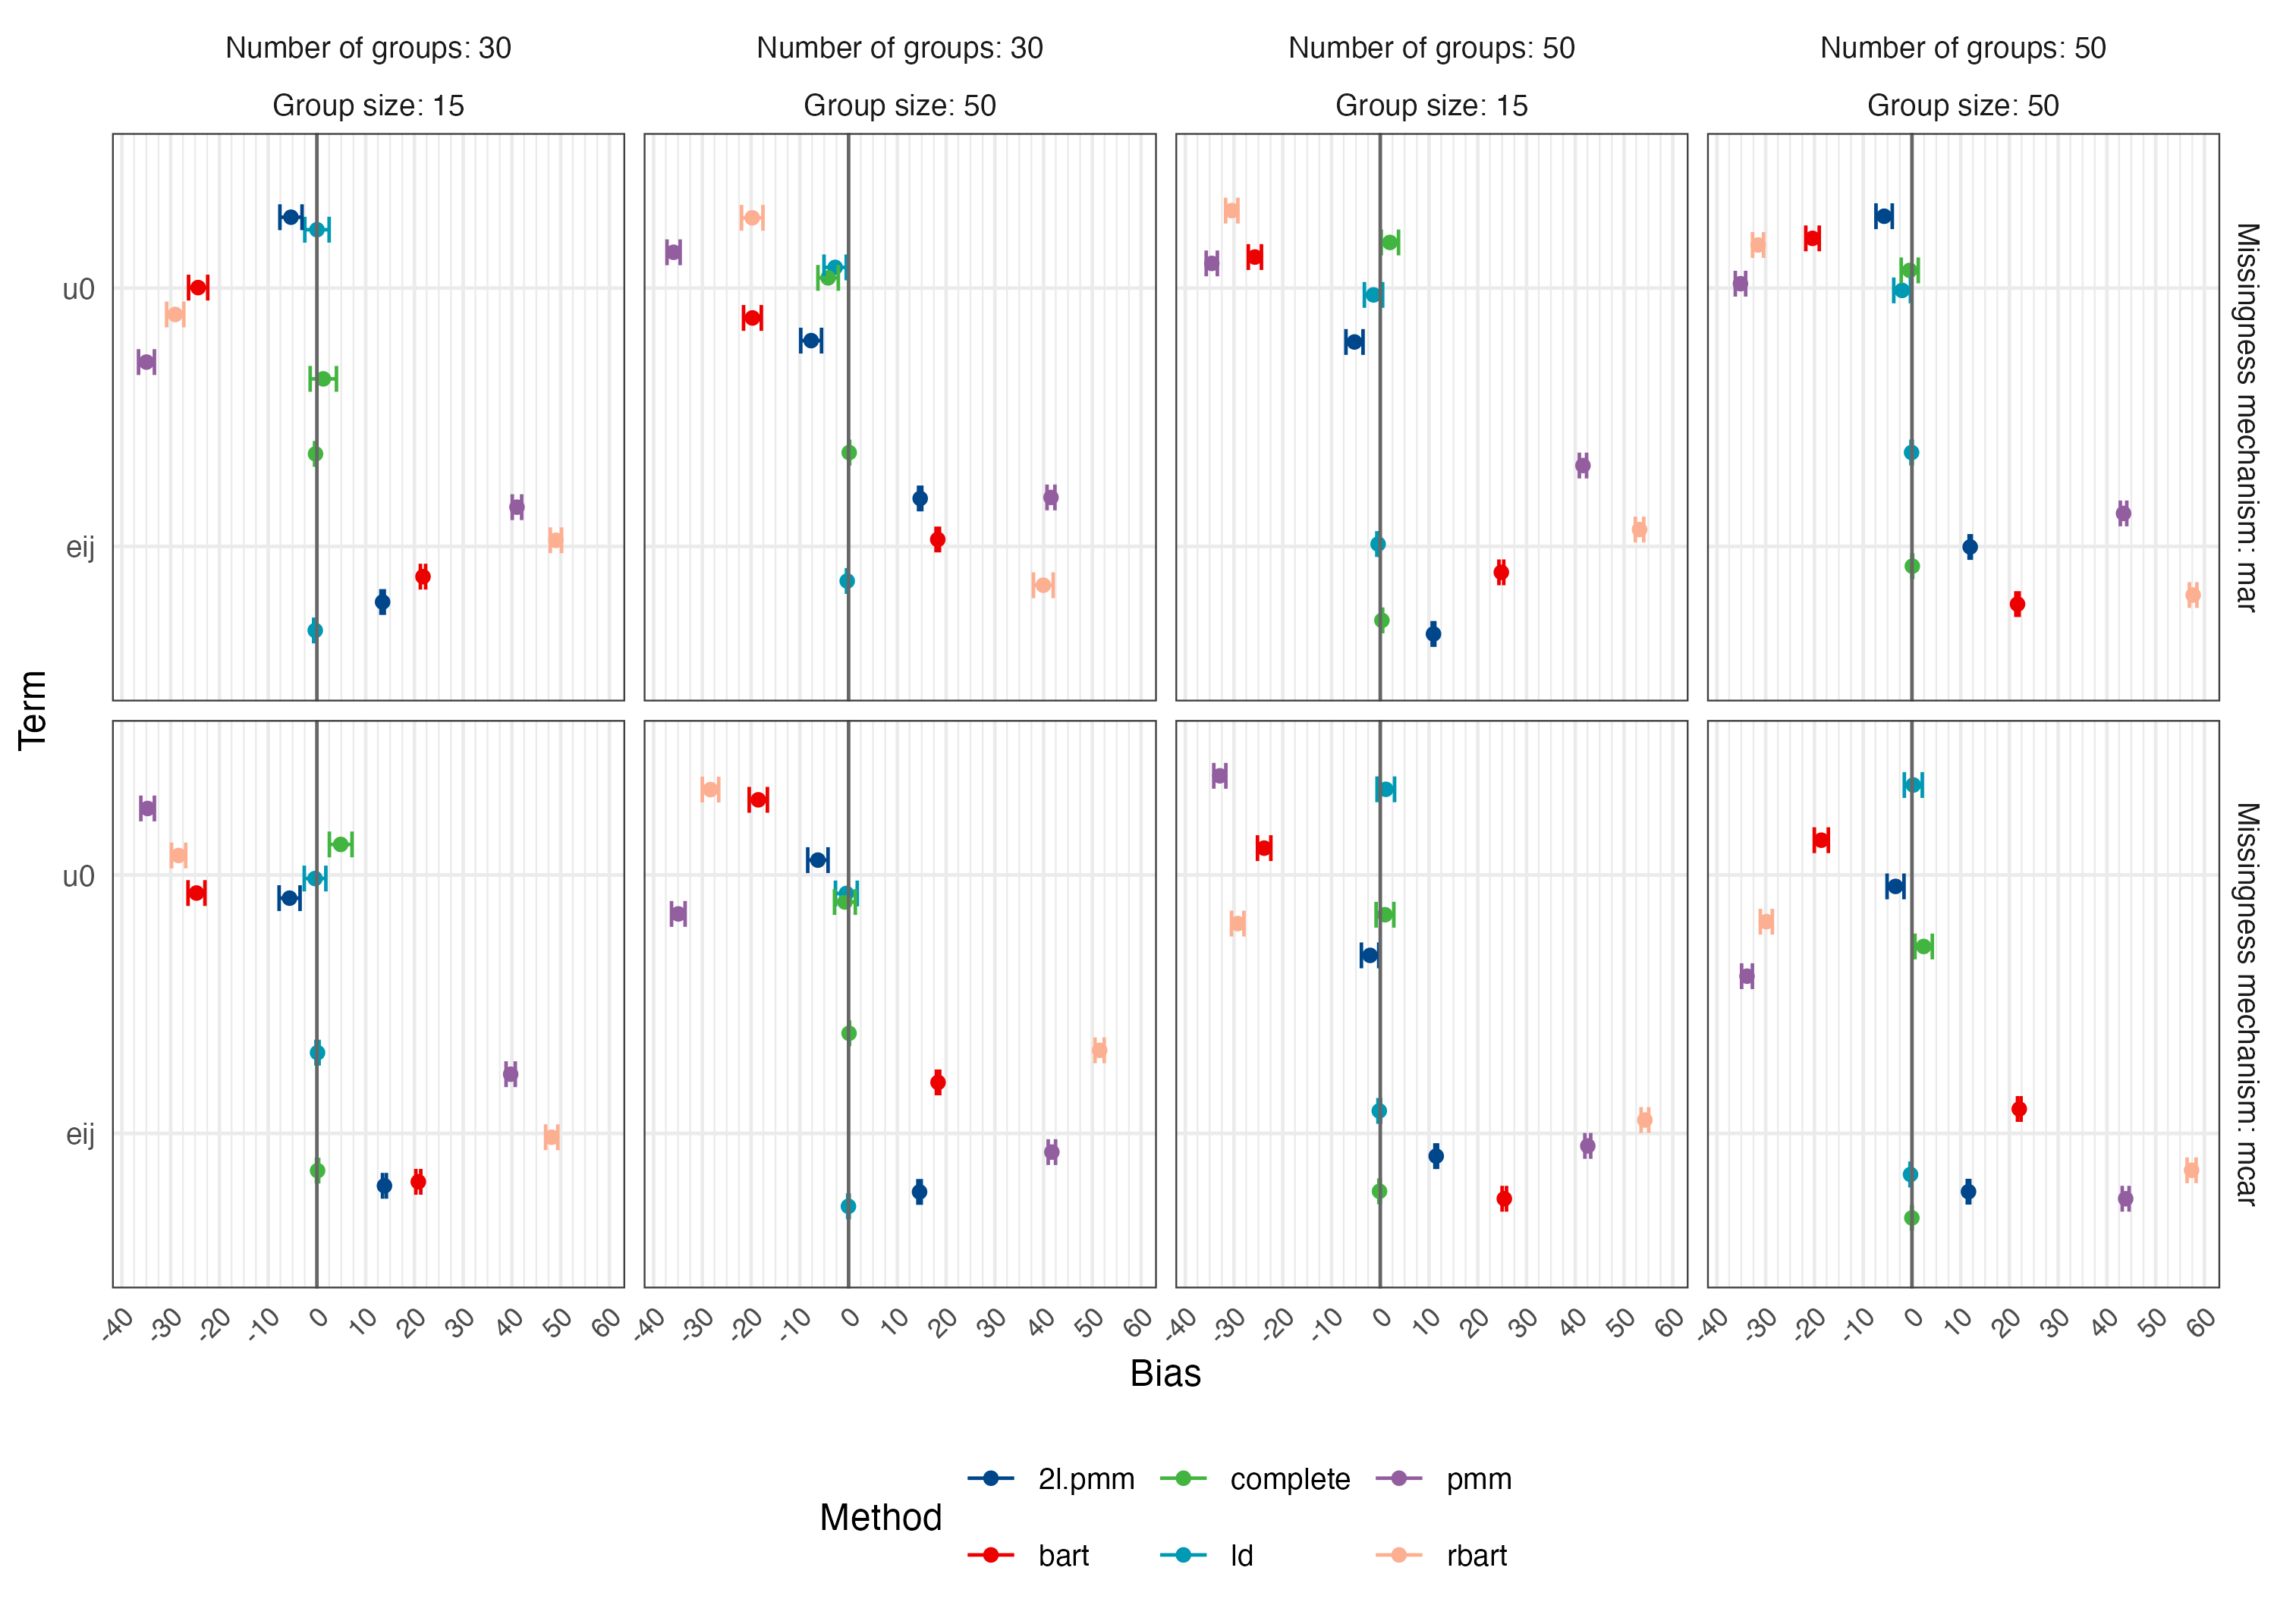
\includegraphics[width=1\textwidth]{bias2.png}
    \caption{Bias of the eij and u0}
    \label{fig:bias2}
\end{figure}

\subsection{Coverage}
Figures \ref{fig:coveragelevel1} and \ref{fig:coveragelevel2} show the coverage of the 95\% confidence intervals of the estimates of the linear mixed model --- the overall intercept; the level-1 effects; and the level-2 effects --- for all imputation methods in consideration with Monte Carlo SE.

First, the estimates of the level-1 fixed effects --- the overal intercept, $\gamma_{00}$ and level-1 effects $\gamma_{10}:\gamma_{70}$ --- will be considered in terms of coverage. Then, the level-2 effects --- $\gamma_{01}$ and $\gamma_{02}$ --- and cross-leven interactions --- $\gamma_{11}, \gamma{21}$ and $\gamma_{32}$ will be considered.

Figure \ref{fig:coveragelevel1} shows that the coverage of the overall intercept, $\gamma_{00}$, is best for imputation method 2l.PMM when the data is MAR. However, when the data is MCAR, stan4bart performs best. Namely, 2l.PMM shows slight undercoverage in the smallest sample size when the data is MCAR and stan4bart shows more flucutations in coverage when the data is MAR. PMM shows undercoverage for all conditions. R-BART also shows consitent undercoverage of the intercept for all conditions except with 30 groups of size 15 when the data is MAR. BART undercovers the intercept for all conditions when the data is MAR, but shows acceptable coverage when the data is MCAR and there are 50 groups. 

Next, the coverage of the level-1 effects in figure \ref{fig:coveragelevel1} shows that 2l.PMM performs best out of all imputation methods for all conditions. Stan4bart also shows a good performance in terms of coverage, however, it regularly overcovers and sometimes undercovers the level-1 effects. PMM at times shows under- or overcoverage, while BART more consistently shows undercoverage. R-BART has most fluctuations in coverage: when group sizes are 50, it shows undercoverage as low as around 47,5\% and overcoverage as high as around 98\%.

% \begin{figure}[H]
%     \centering
%     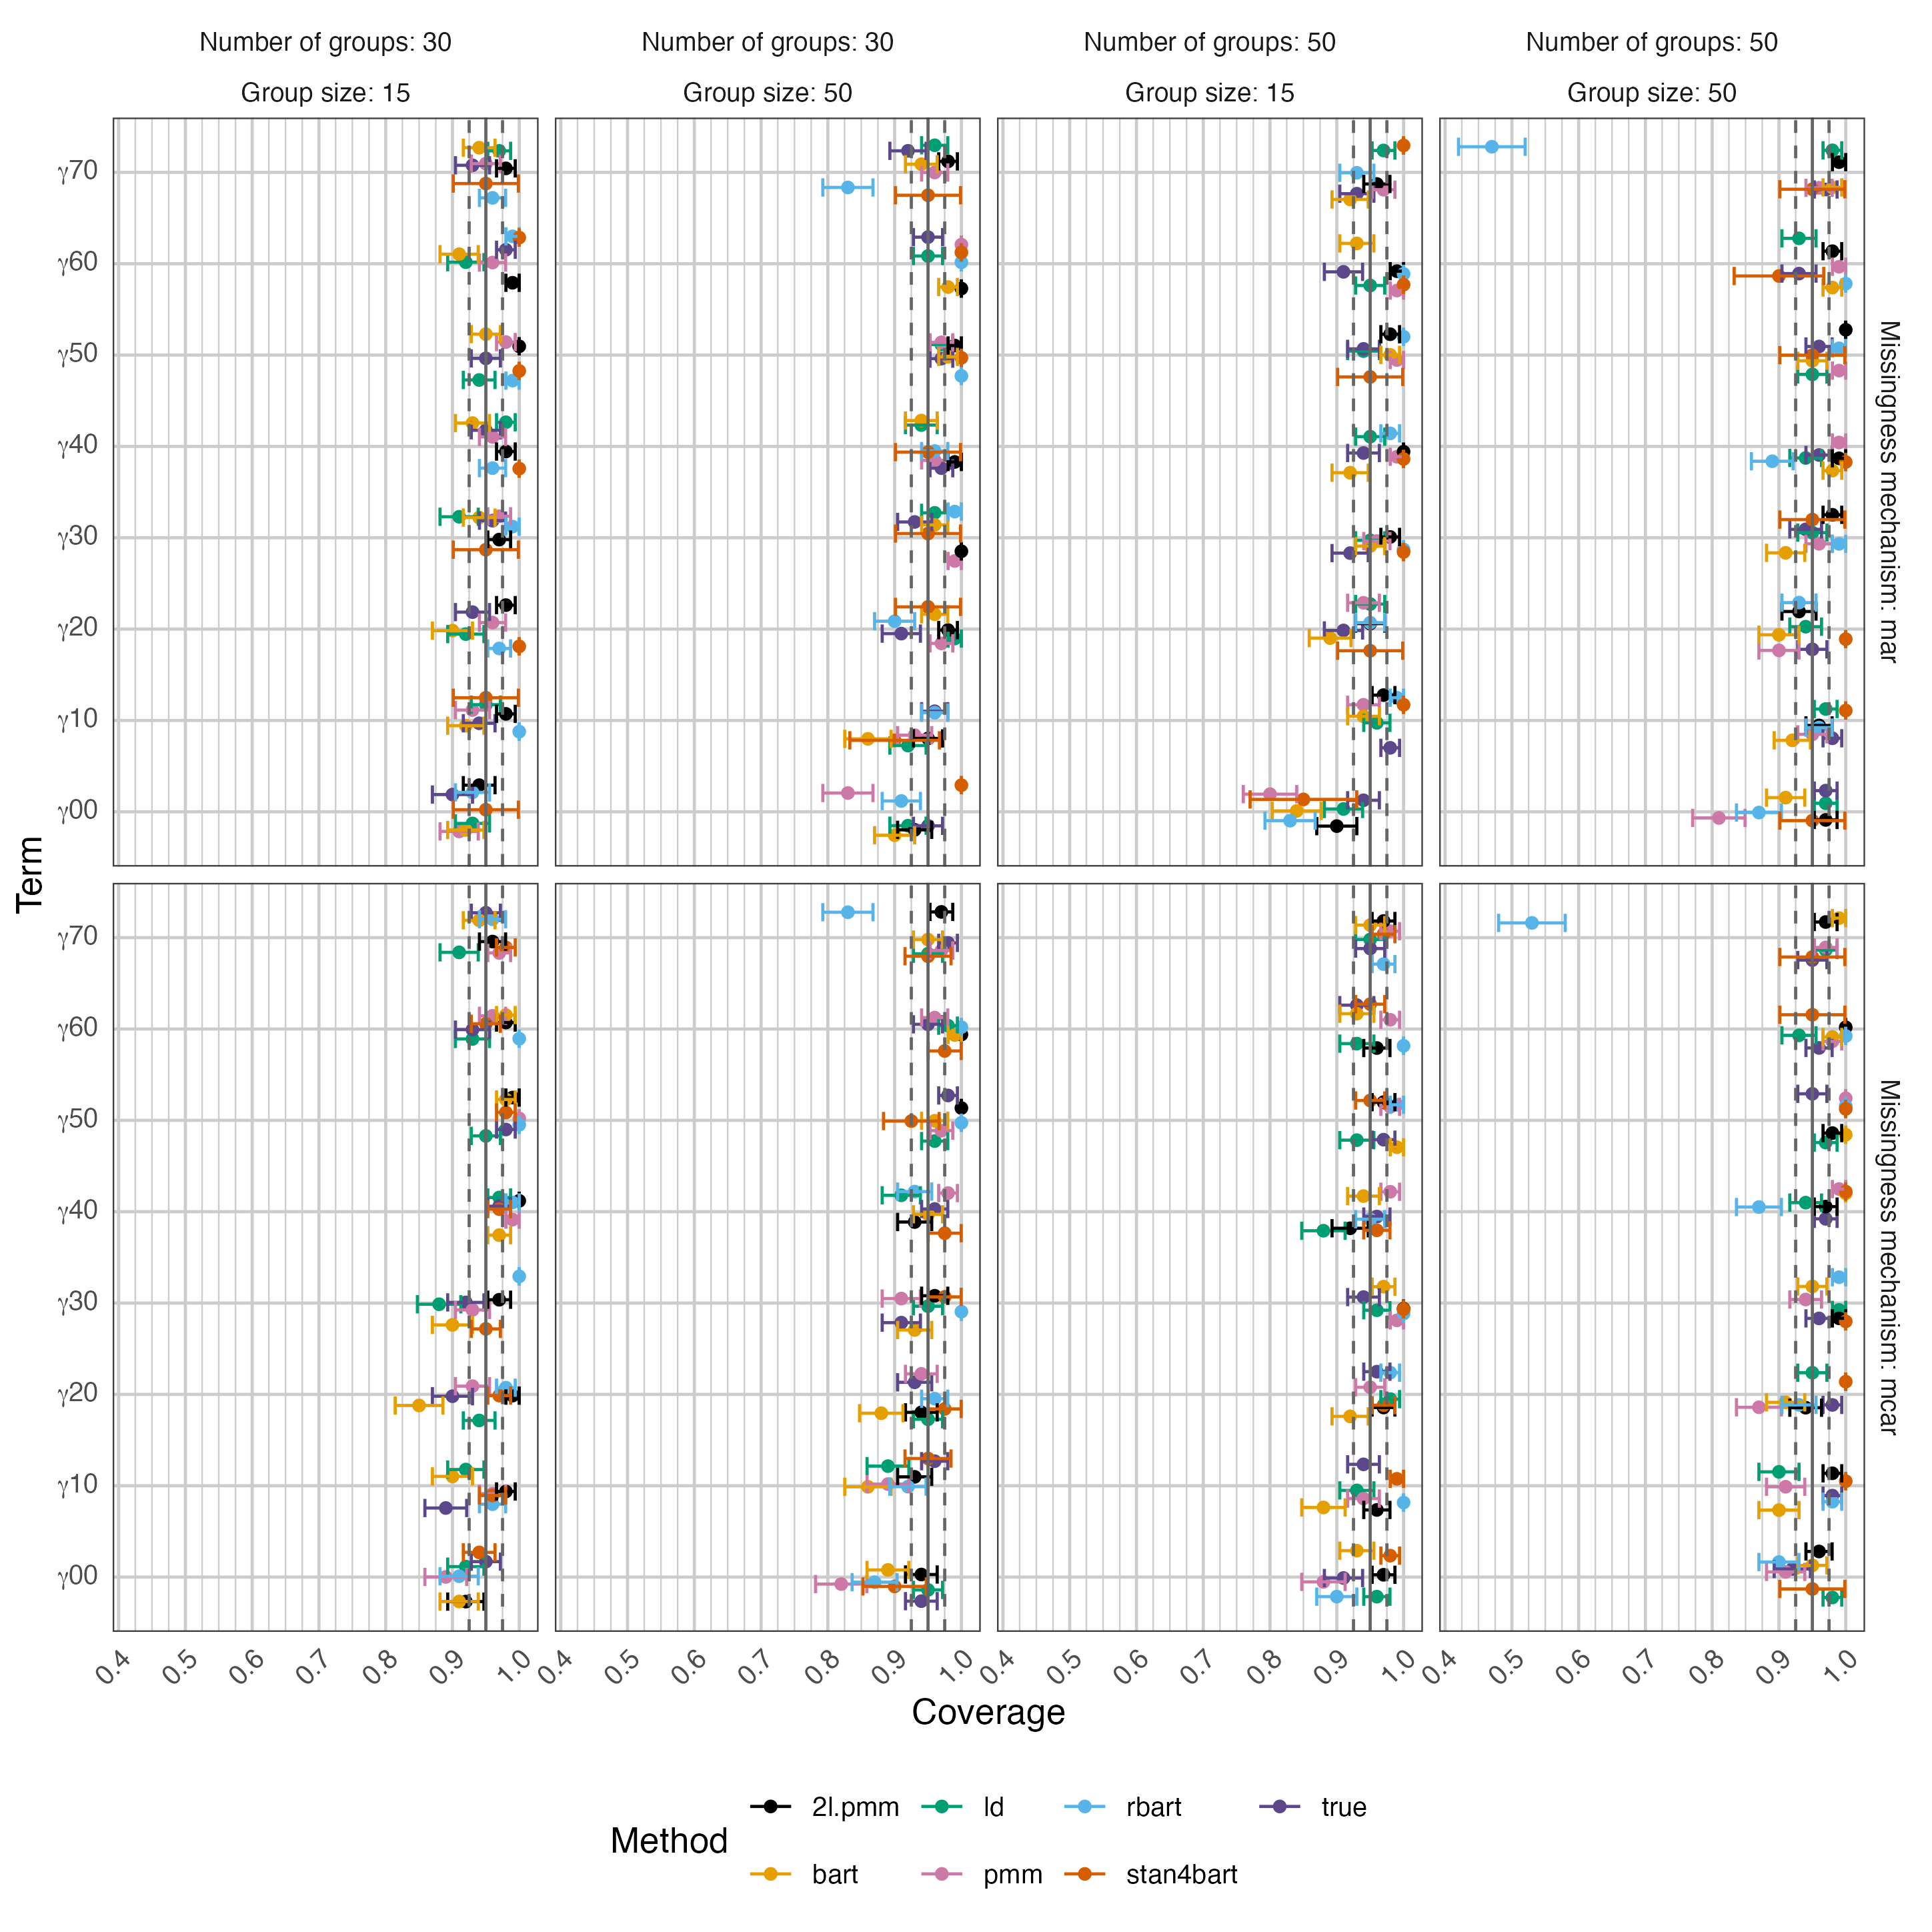
\includegraphics[width=1\textwidth]{coveragelevel1.png}
%     \caption{Coverage of the estimates}
%     \label{fig:coveragelevel1}
% \end{figure}

Lastly, the coverage of the level-2 effects and cross-level interactions in figure \ref{fig:coveragelevel2} shows that BART has the overall worst coverage for all conditions, with coverages ranging from 65\% to 82.5\%. PMM also routinely undercovers the level-2 effects, which worsens with group sizes of 50. R-BART tends to overcover the level-2 effects, but undercovers at times as well the level-2 effect. Overall, 2l.PMM demonstrates the best coverage, despite exhibiting slight undercoverage when the data is MAR and there are 50 groups. 

2l.PMM also has the best coverage of the cross-level interactions out of the imputation methods. Albeit showing a slight under- or overcoverage at times. Listwise deletion also performs considerably good, showing better coverage when the data is MAR compared to MCAR. When the group size is 15, PMM; BART; and R-BART, show an acceptable coverage --- sometimes slightly under- or overcovering the cross-level interactions ---, but considerable undercoverage when the group size is increased to 50. Stan4bart has the worst coverage of the cross-level interactions: showing considerable undercoverage for all conditions, especially when the group size is increased to 50.

\begin{figure}[H]
    \centering
    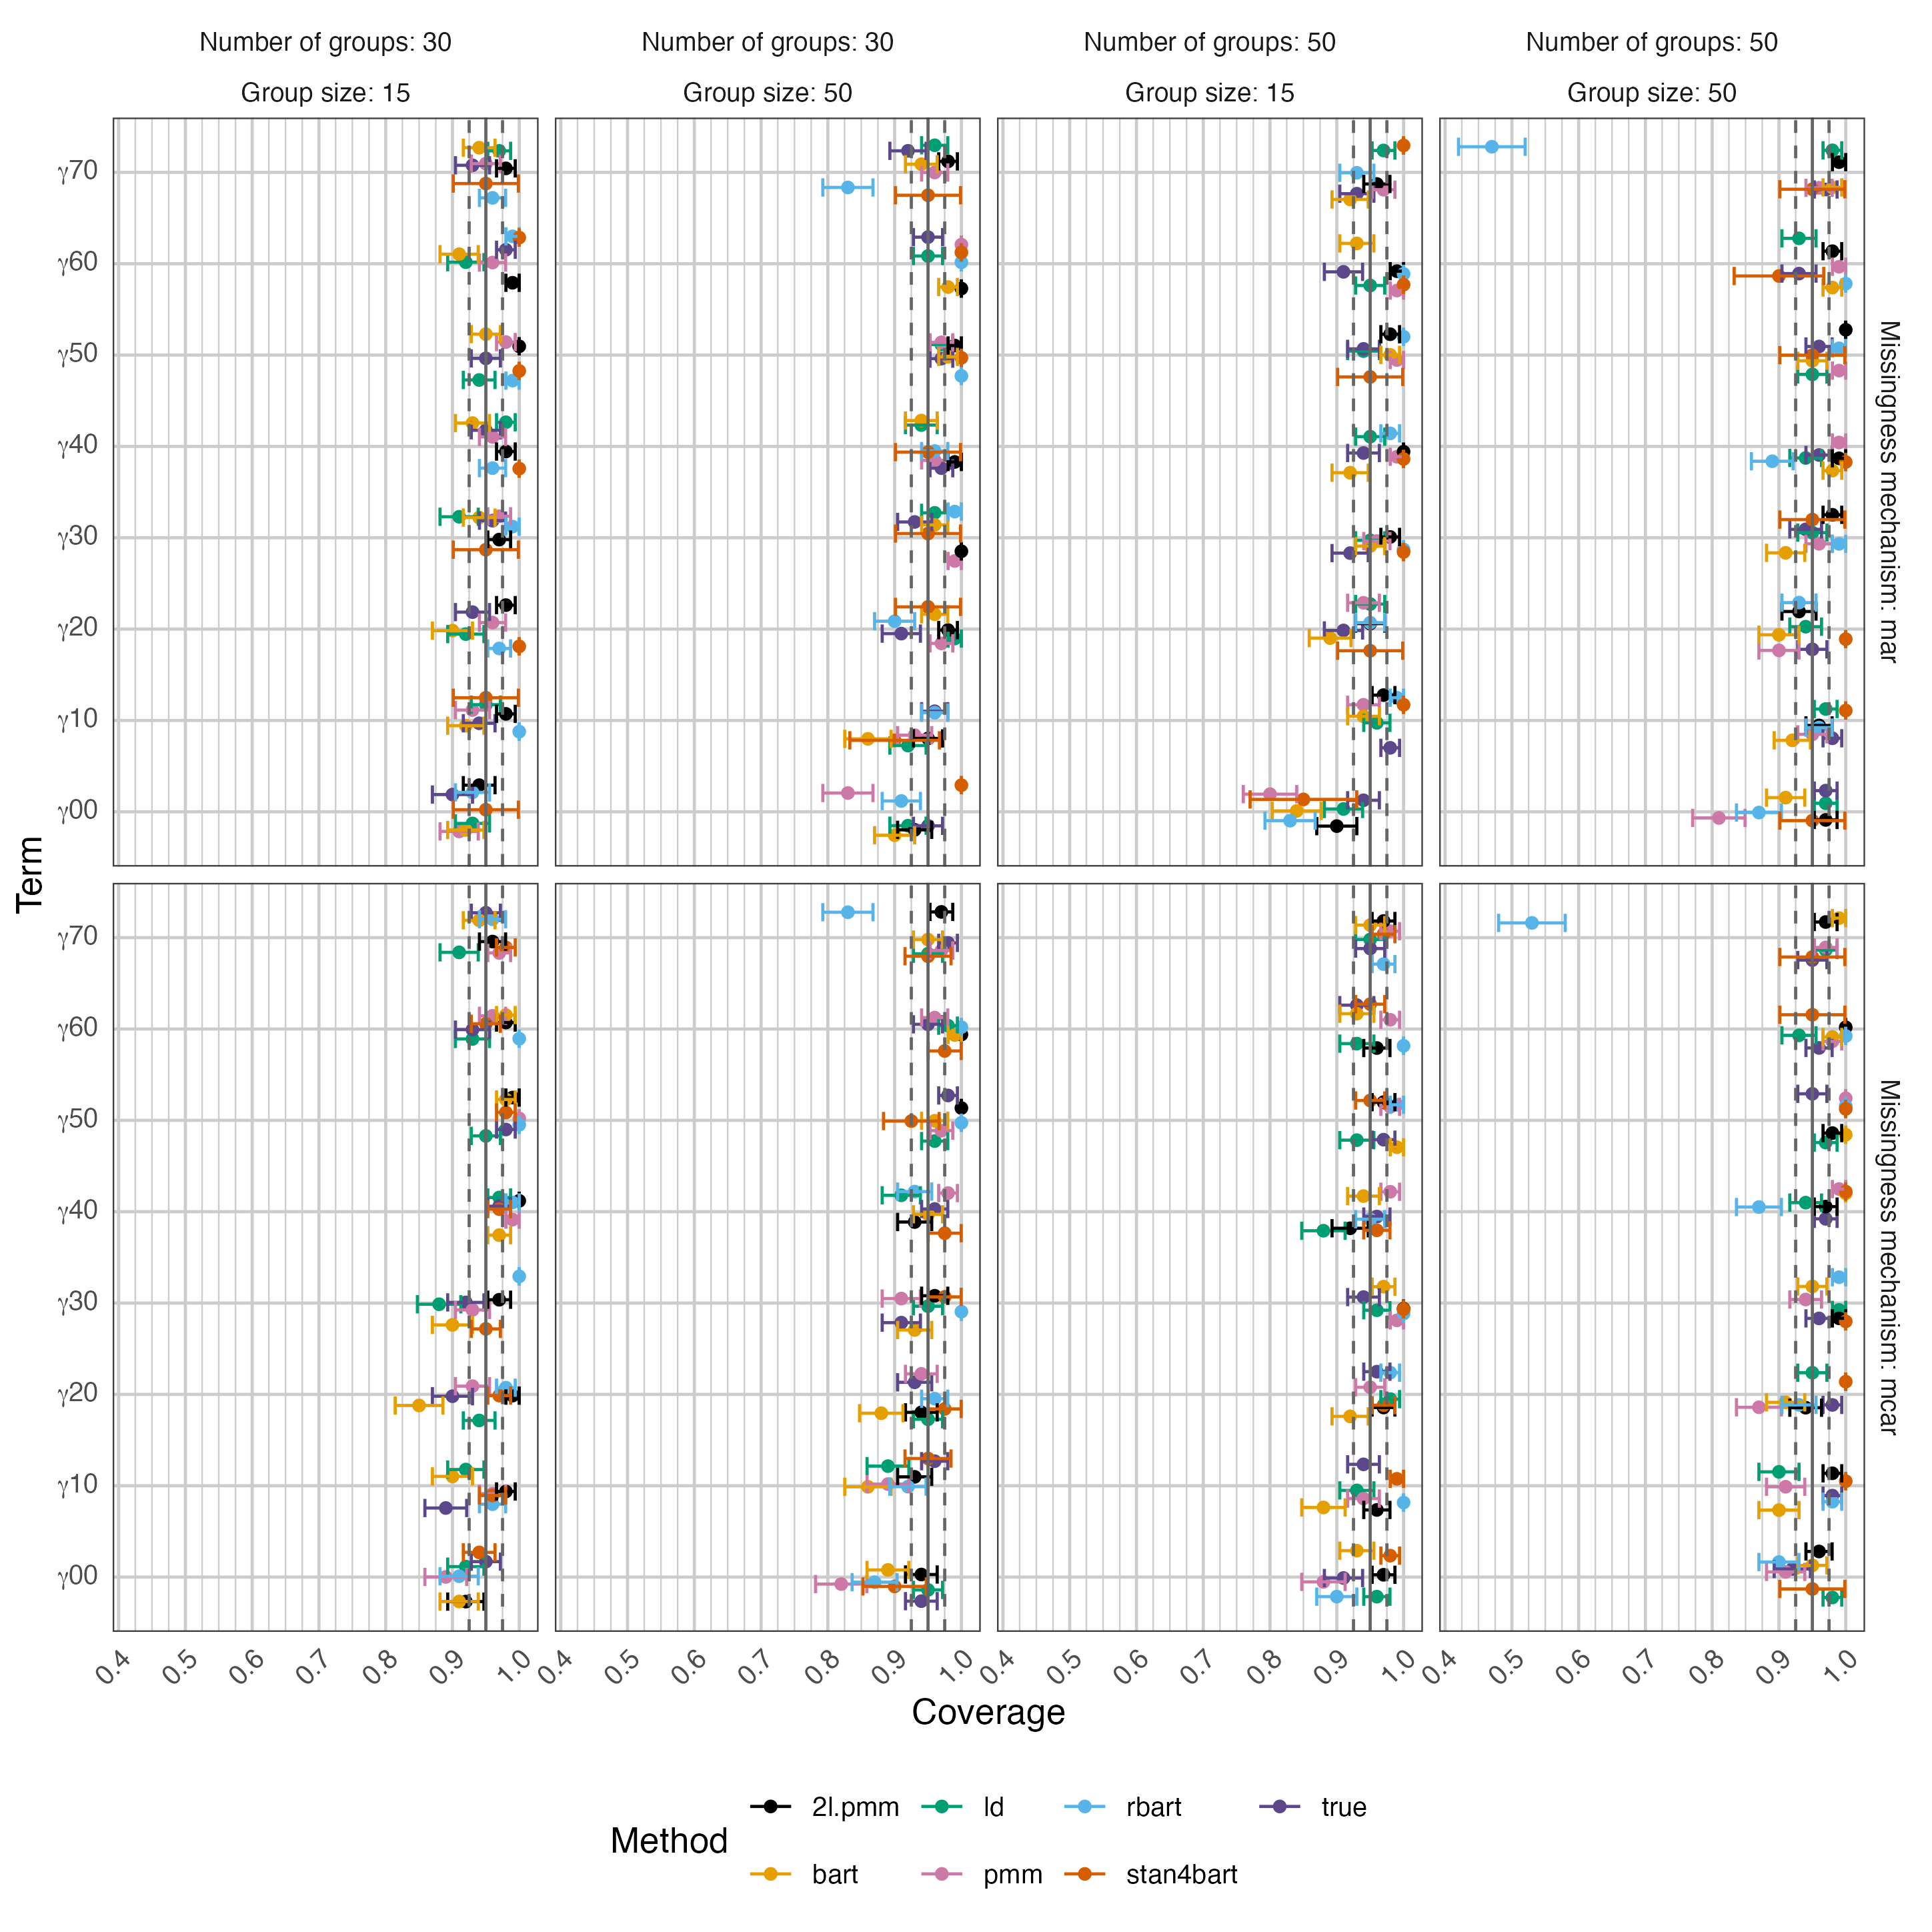
\includegraphics[width=1\textwidth]{coveragelevel1.png}
    \caption{Coverage of the 95\% confidence intervals of the intercept and level-1 effects of the linear mixed model with respective Monte Carlo SE for all simulated datasets over 100 simulations with ICC = .5. The solid line represents the nominal 95\% coverage, and the dashed lines at .925 and .975 represent the liberal criterion from \citet{bradley1978}.}
    \label{fig:coveragelevel1}
\end{figure}

\begin{figure}[H]
    \centering
    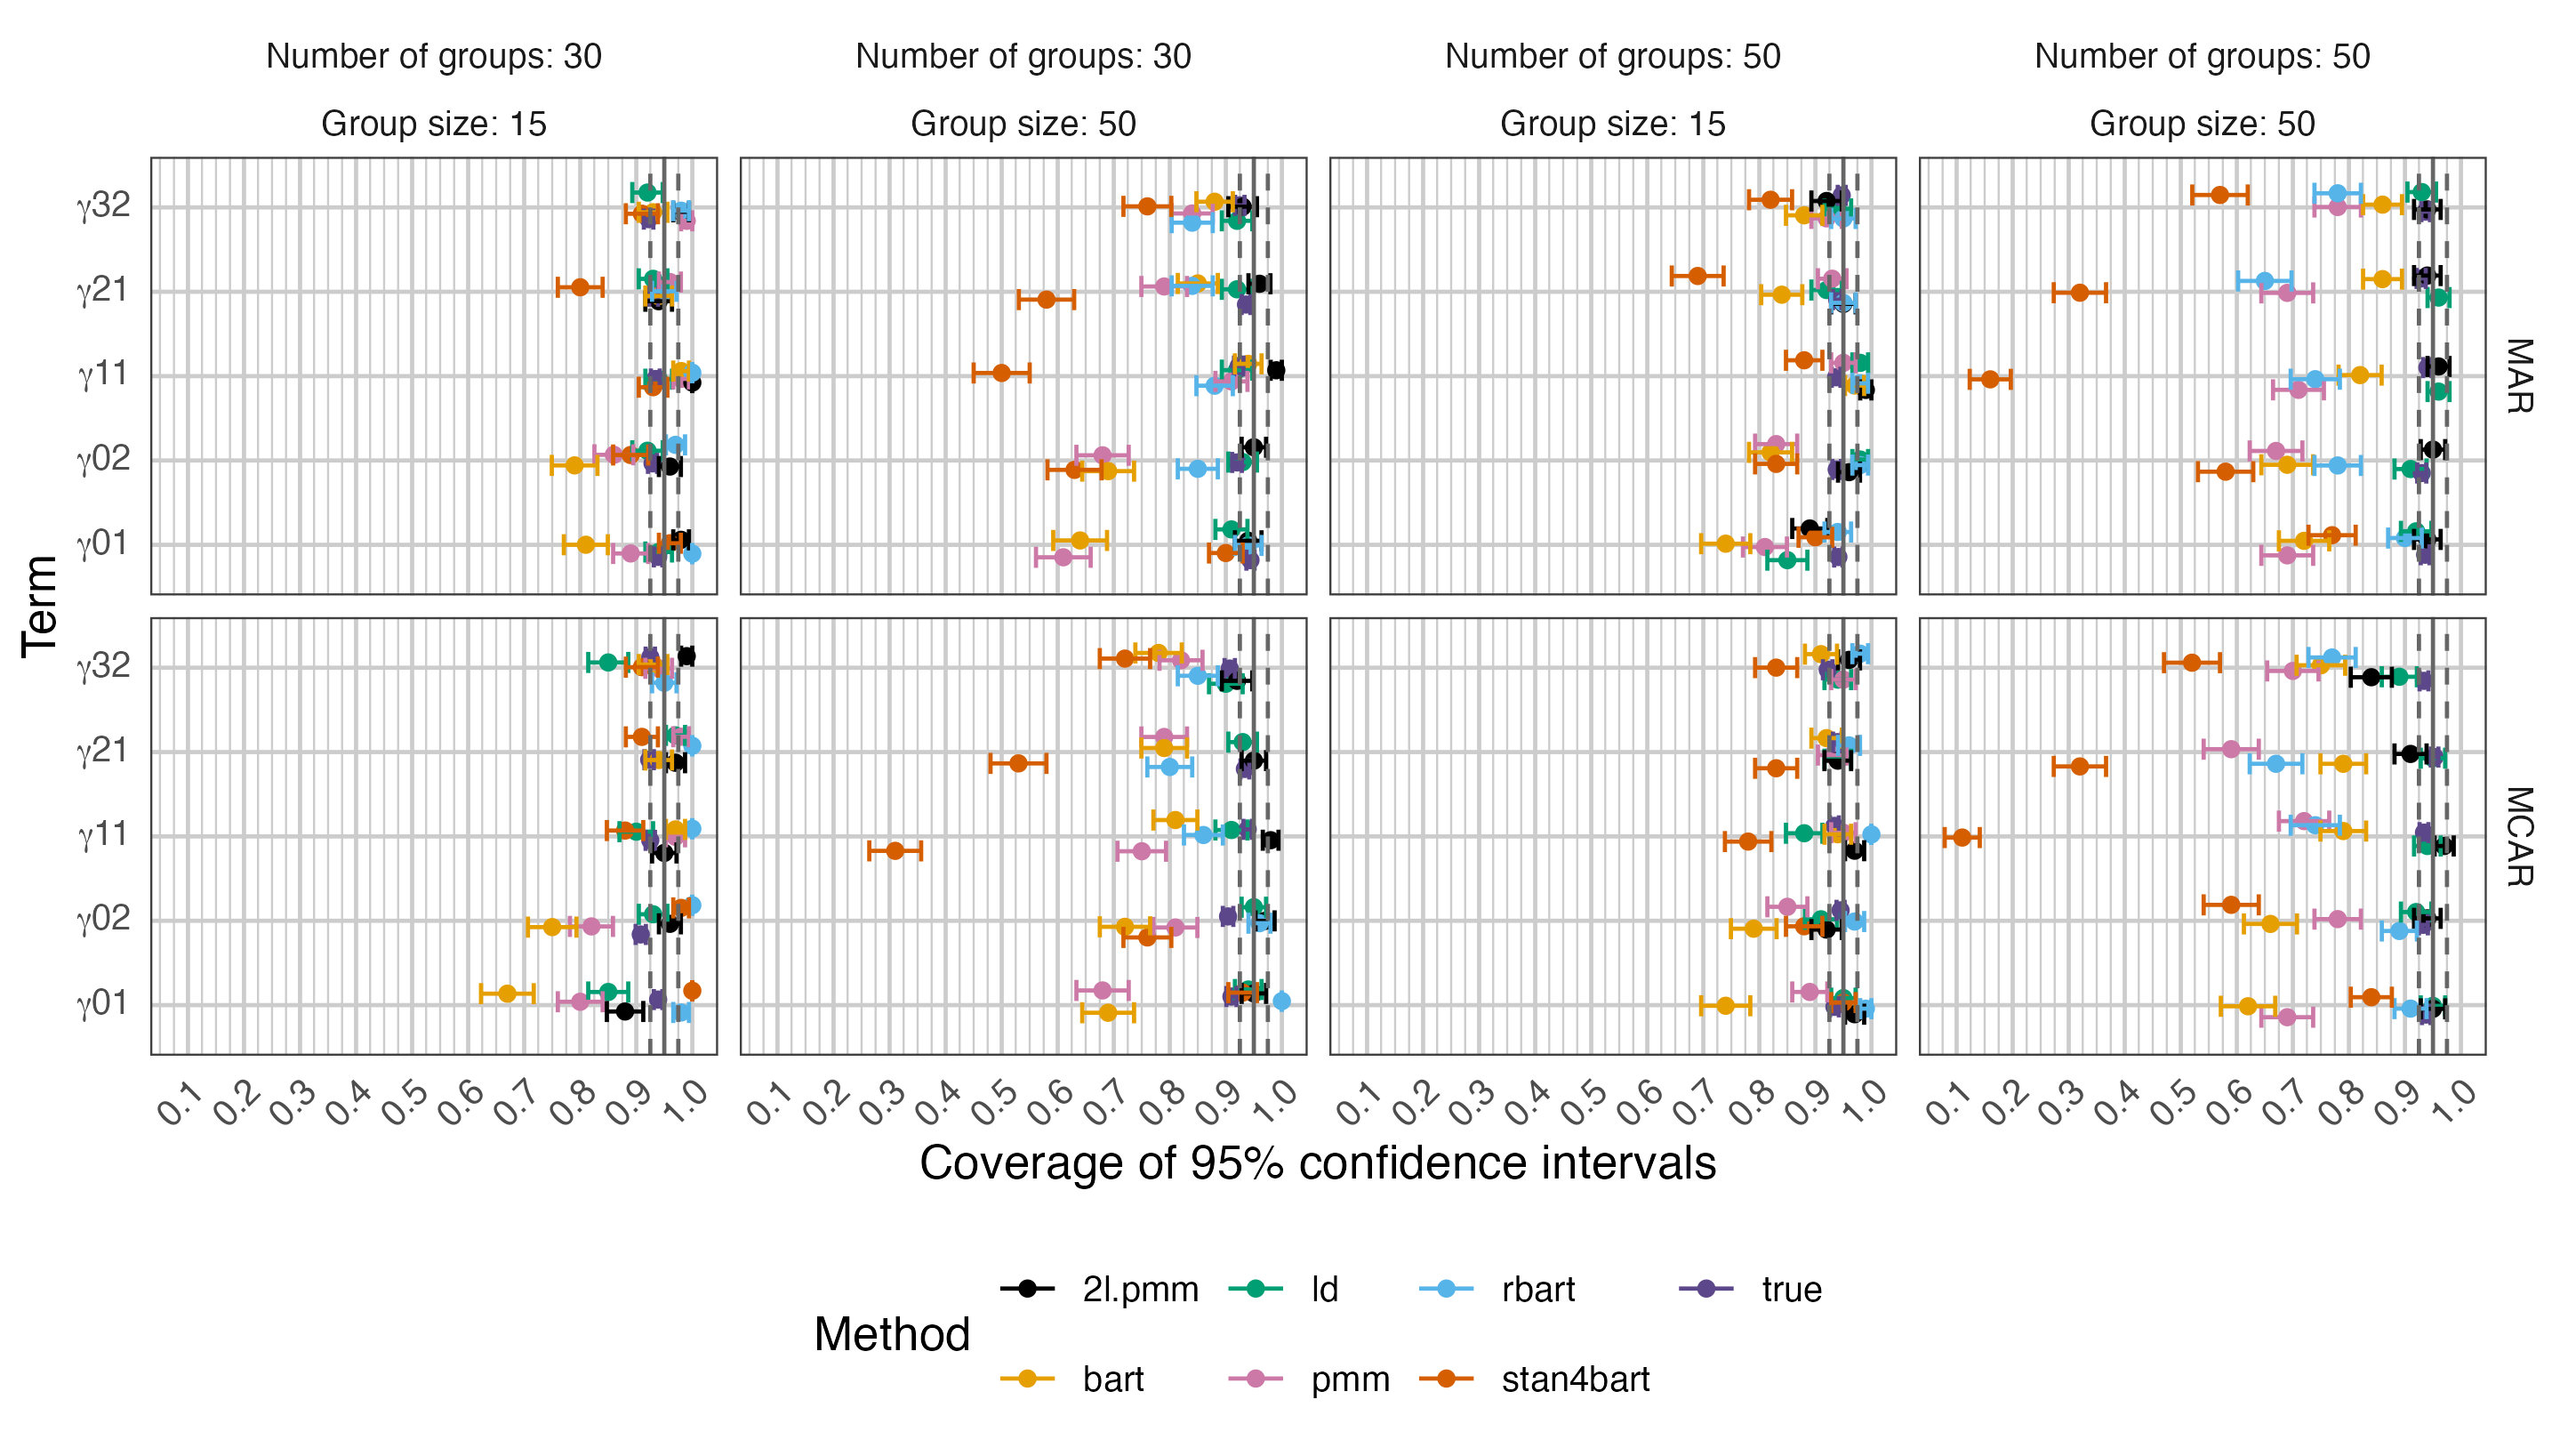
\includegraphics[width=1\textwidth]{coveragelevel2.png}
    \caption{Coverage of the 95\% confidence intervals of the level-2 and cross-level effects of the linear mixed model with respective Monte Carlo SE for all simulated datasets over 100 simulations with ICC = .5. The solid line represents the nominal 95\% coverage, and the dashed lines at .925 and .975 represent the liberal criterion from \citet{bradley1978}.}
    \label{fig:coveragelevel2}
\end{figure}

\subsection{Confidence interval width}
Figures \ref{fig:ciwintercept}, \ref{fig:ciwlevel1}, and \ref{fig:ciwlevel2} show the 95\% confidence interval width of the estimates of the linear mixed model --- the overall intercept; the level-1 effects; and the level-2 effects --- for all imputation methods in consideration.

First, the estimates of the level-1 fixed effects --- the overal intercept, $\gamma_{00}$ and level-1 effects, $\gamma_{10}:\gamma_{70}$ --- will be considered in terms of coverage. Then, the level-2 effects --- $\gamma_{01}$ and $\gamma_{02}$ --- and cross-leven interactions --- $\gamma_{11}, \gamma{21}$ and $\gamma_{32}$ will be considered.

Figure \ref{fig:ciwintercept} shows that the confidence interval width of the intercept is smallest for PMM. However, paired with the coverage estimates from figure \ref{fig:coveragelevel1}, PMM seems to be efficient but routinely undercovers the intercept. The same pattern can be seen for BART and R-BART, while showing smaller confidence intervals widths, they routinely undercover the intercept. 2l.PMM, stan4bart and listwise deletion show larger confidence interval widths --- somewhat mimicking the ``true'' data with 0\% missing values --- oft paired with acceptable coverage.

% \begin{figure}[H]
%     \centering
%     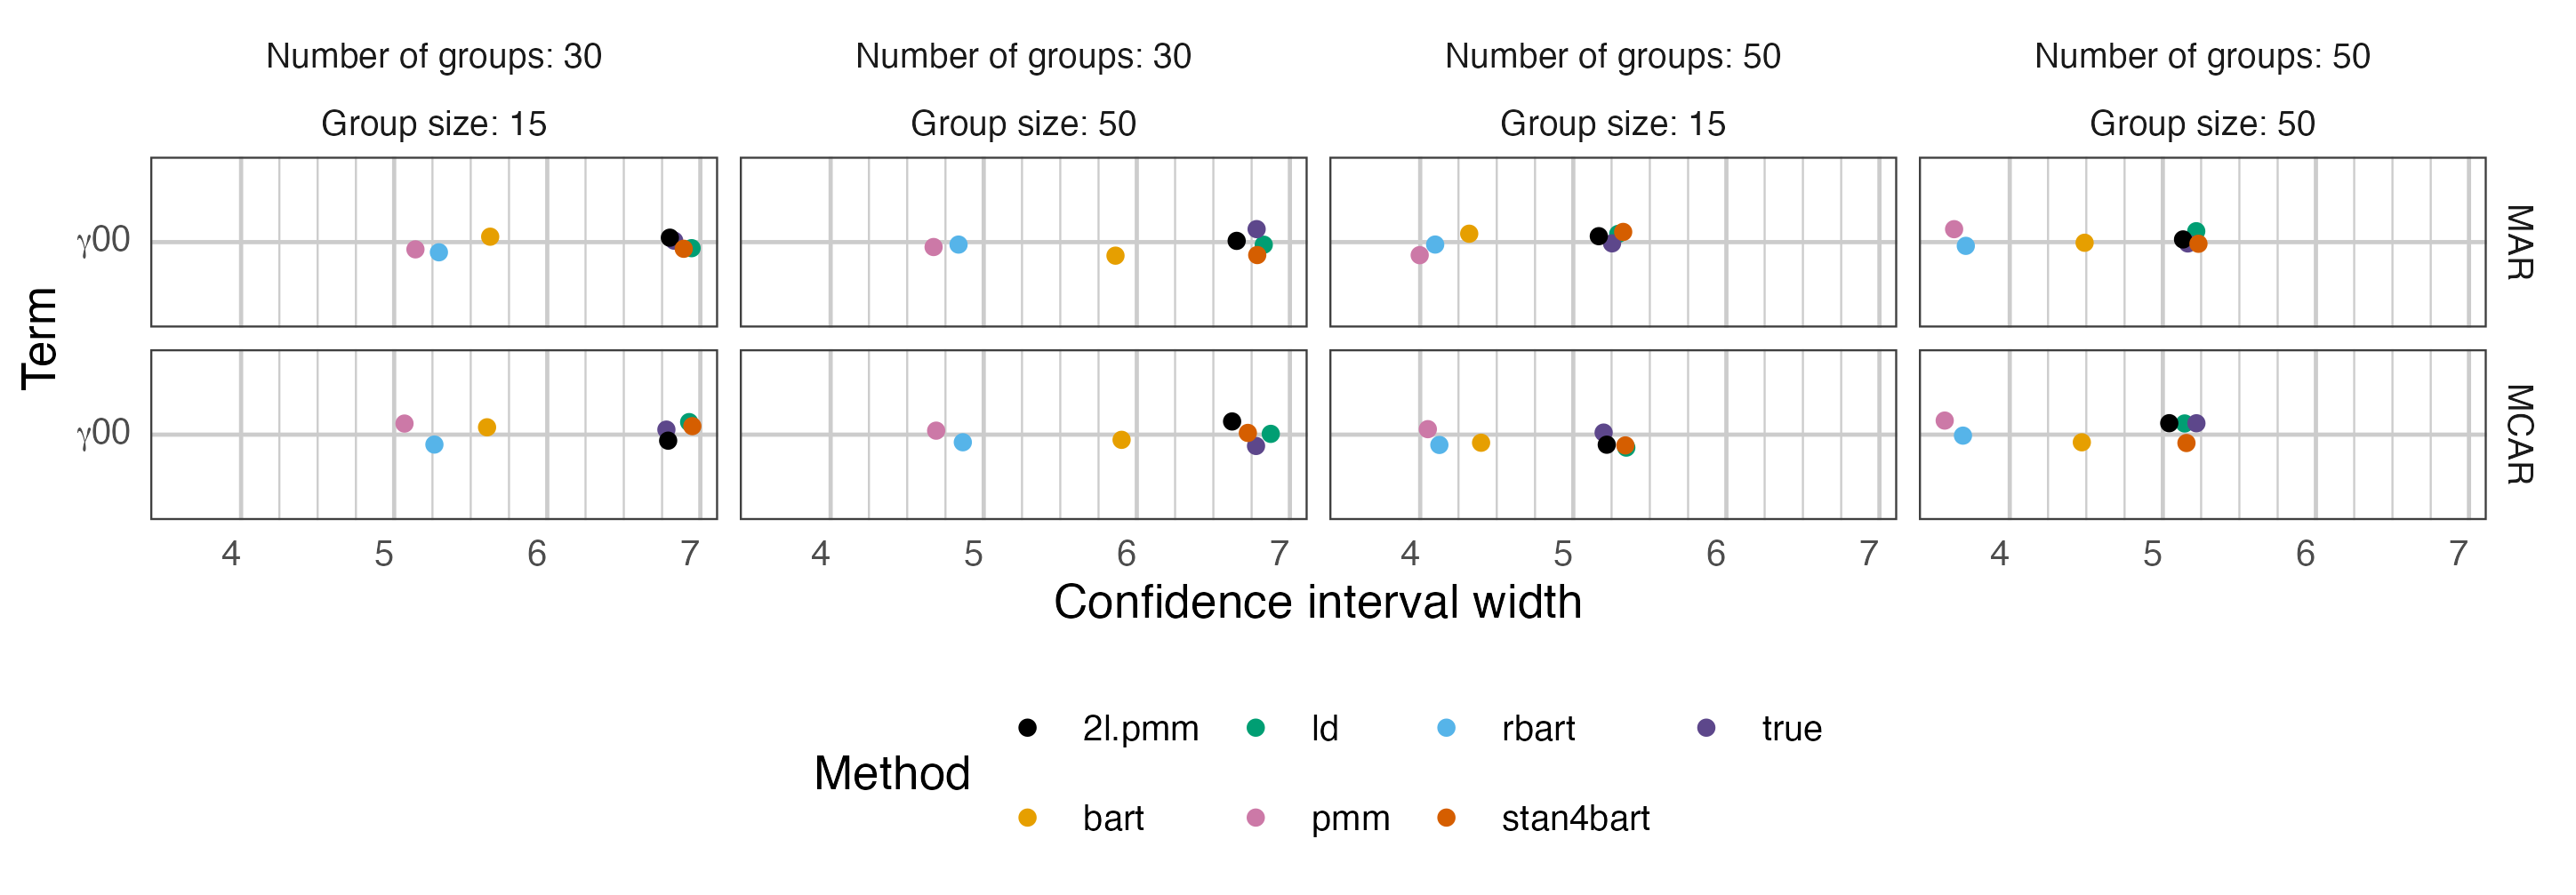
\includegraphics[width=1\textwidth]{ciwintercept.png}
%     \caption{Confidence interval width of the estimates}
%     \label{fig:ciwintercept}
% \end{figure}

For the level-1 effects, $\gamma_{10}:\gamma_{70}$, the confidence interval width of the ``true'' data with 0\% missing values is oft smallest. Listwise deletion and stan4bart are closest in mimicking the width of the ``true'' data and figure \ref{fig:coveragelevel1} shows generally show acceptable coverage of the level-1 effects. 2l.PMM and BART have overall slightly larger confidence intervals, and, as mentoined before, 2l.PMM has the best coverage of the level-1 effects while BART shows more undercoverage. Then, PMM and R-BART show the largest confidence intervals. PMM shows both under- and overcoverage in figure \ref{fig:coveragelevel1}, while R-BART shows considerable undercoverage when its confidence intervals are smallest and overcoverage when its confidence intervals are largest --- for example for effect $\gamma_{70}$ and $\gamma_{60}$ when the data is MAR with 50 groups of 50. Lastly, the confidence interval width for all methods decreases towards the ``true'' data's confidence interval width with an increase in total sample size. 

% \begin{figure}[H]
%     \centering
%     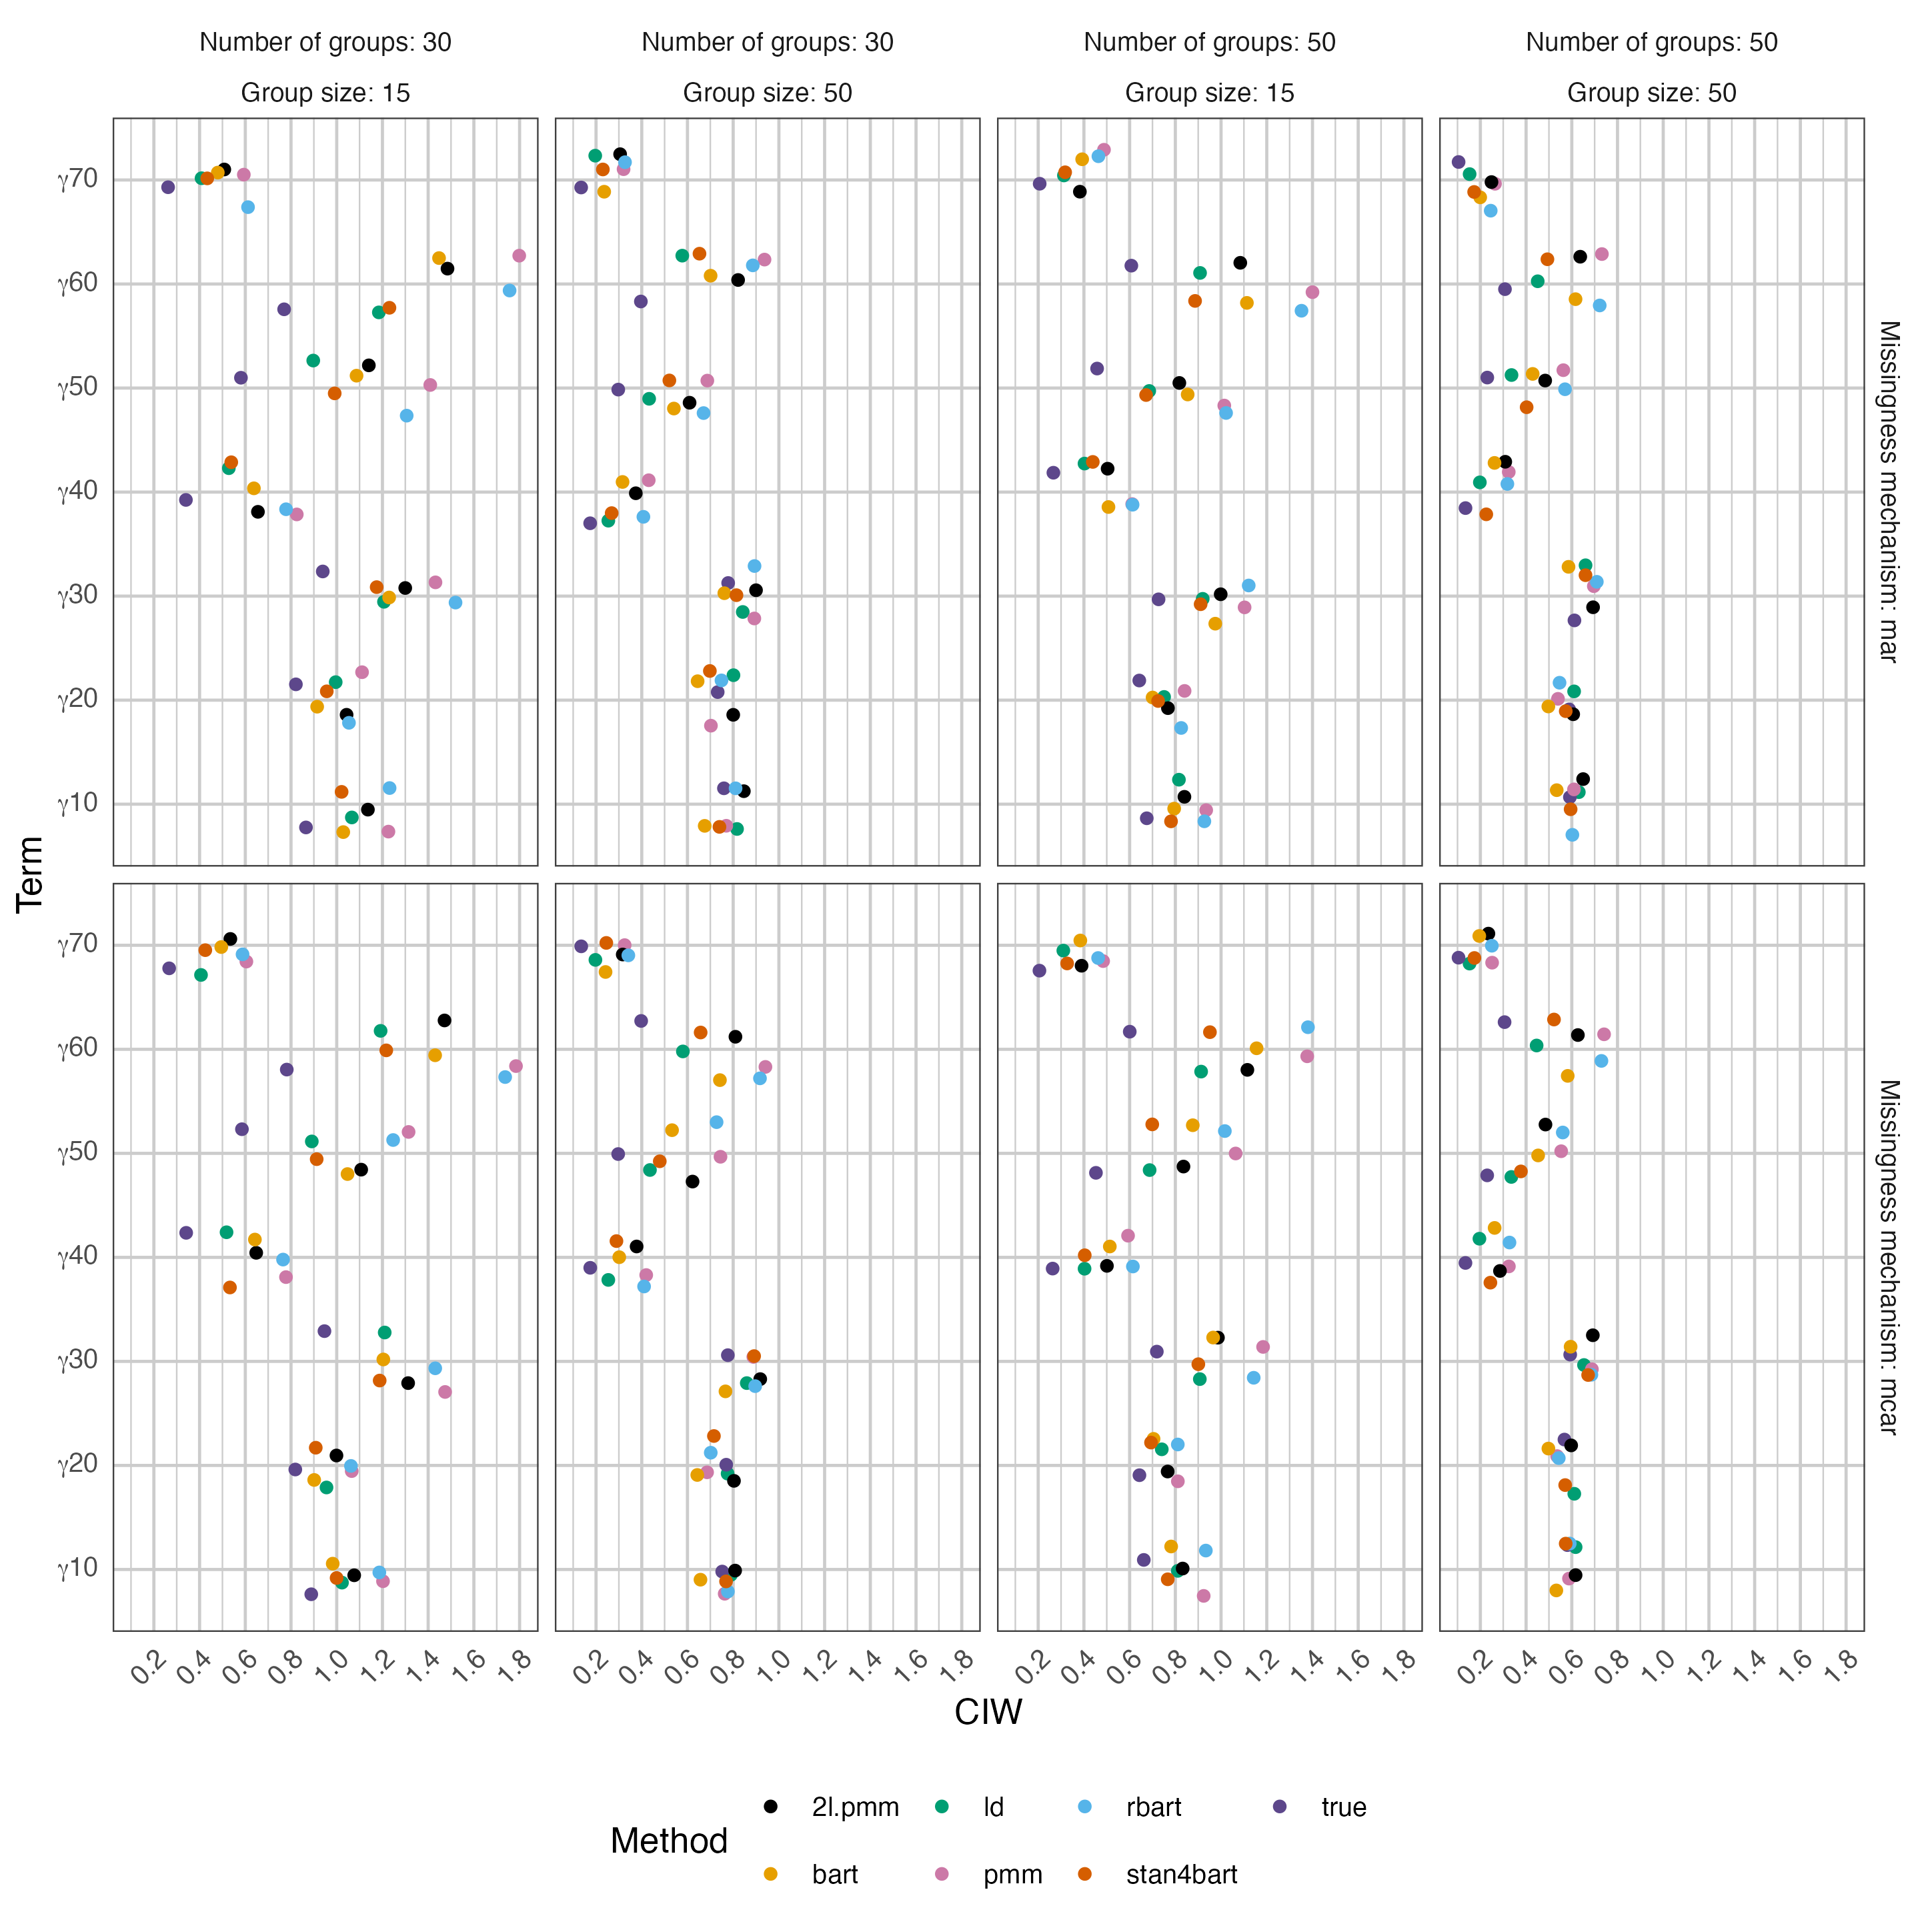
\includegraphics[width=1\textwidth]{ciwlevel1.png}
%     \caption{Confidence interval width of the estimates}
%     \label{fig:ciwlevel1}
% \end{figure}

From figure \ref{fig:ciwlevel2} we can see that 2l.PMM has largest confidence interval width of all imputation methods for the level-2 effects, substantially mimicking the confidence interval from the 0\% missing data. Listwise deletion performs similar to 2l.PMM and the 0\% missing data. The other imputation methods, PMM; BART; R-BART; and stan4bart, show smaller confidence intervals and show a similar pattern in the confidence interval width when the total sample size increases: the confidence interval width decreases leading to more undercoverage --- as can be seen in figure \ref{fig:coveragelevel2}. At the same time, 2l.PMM and listwise deletion show a decrease in width when there are more groups in the data, which is a pattern mirrored by the ``true'' data as well. 

% \begin{figure}[H]
%     \centering
%     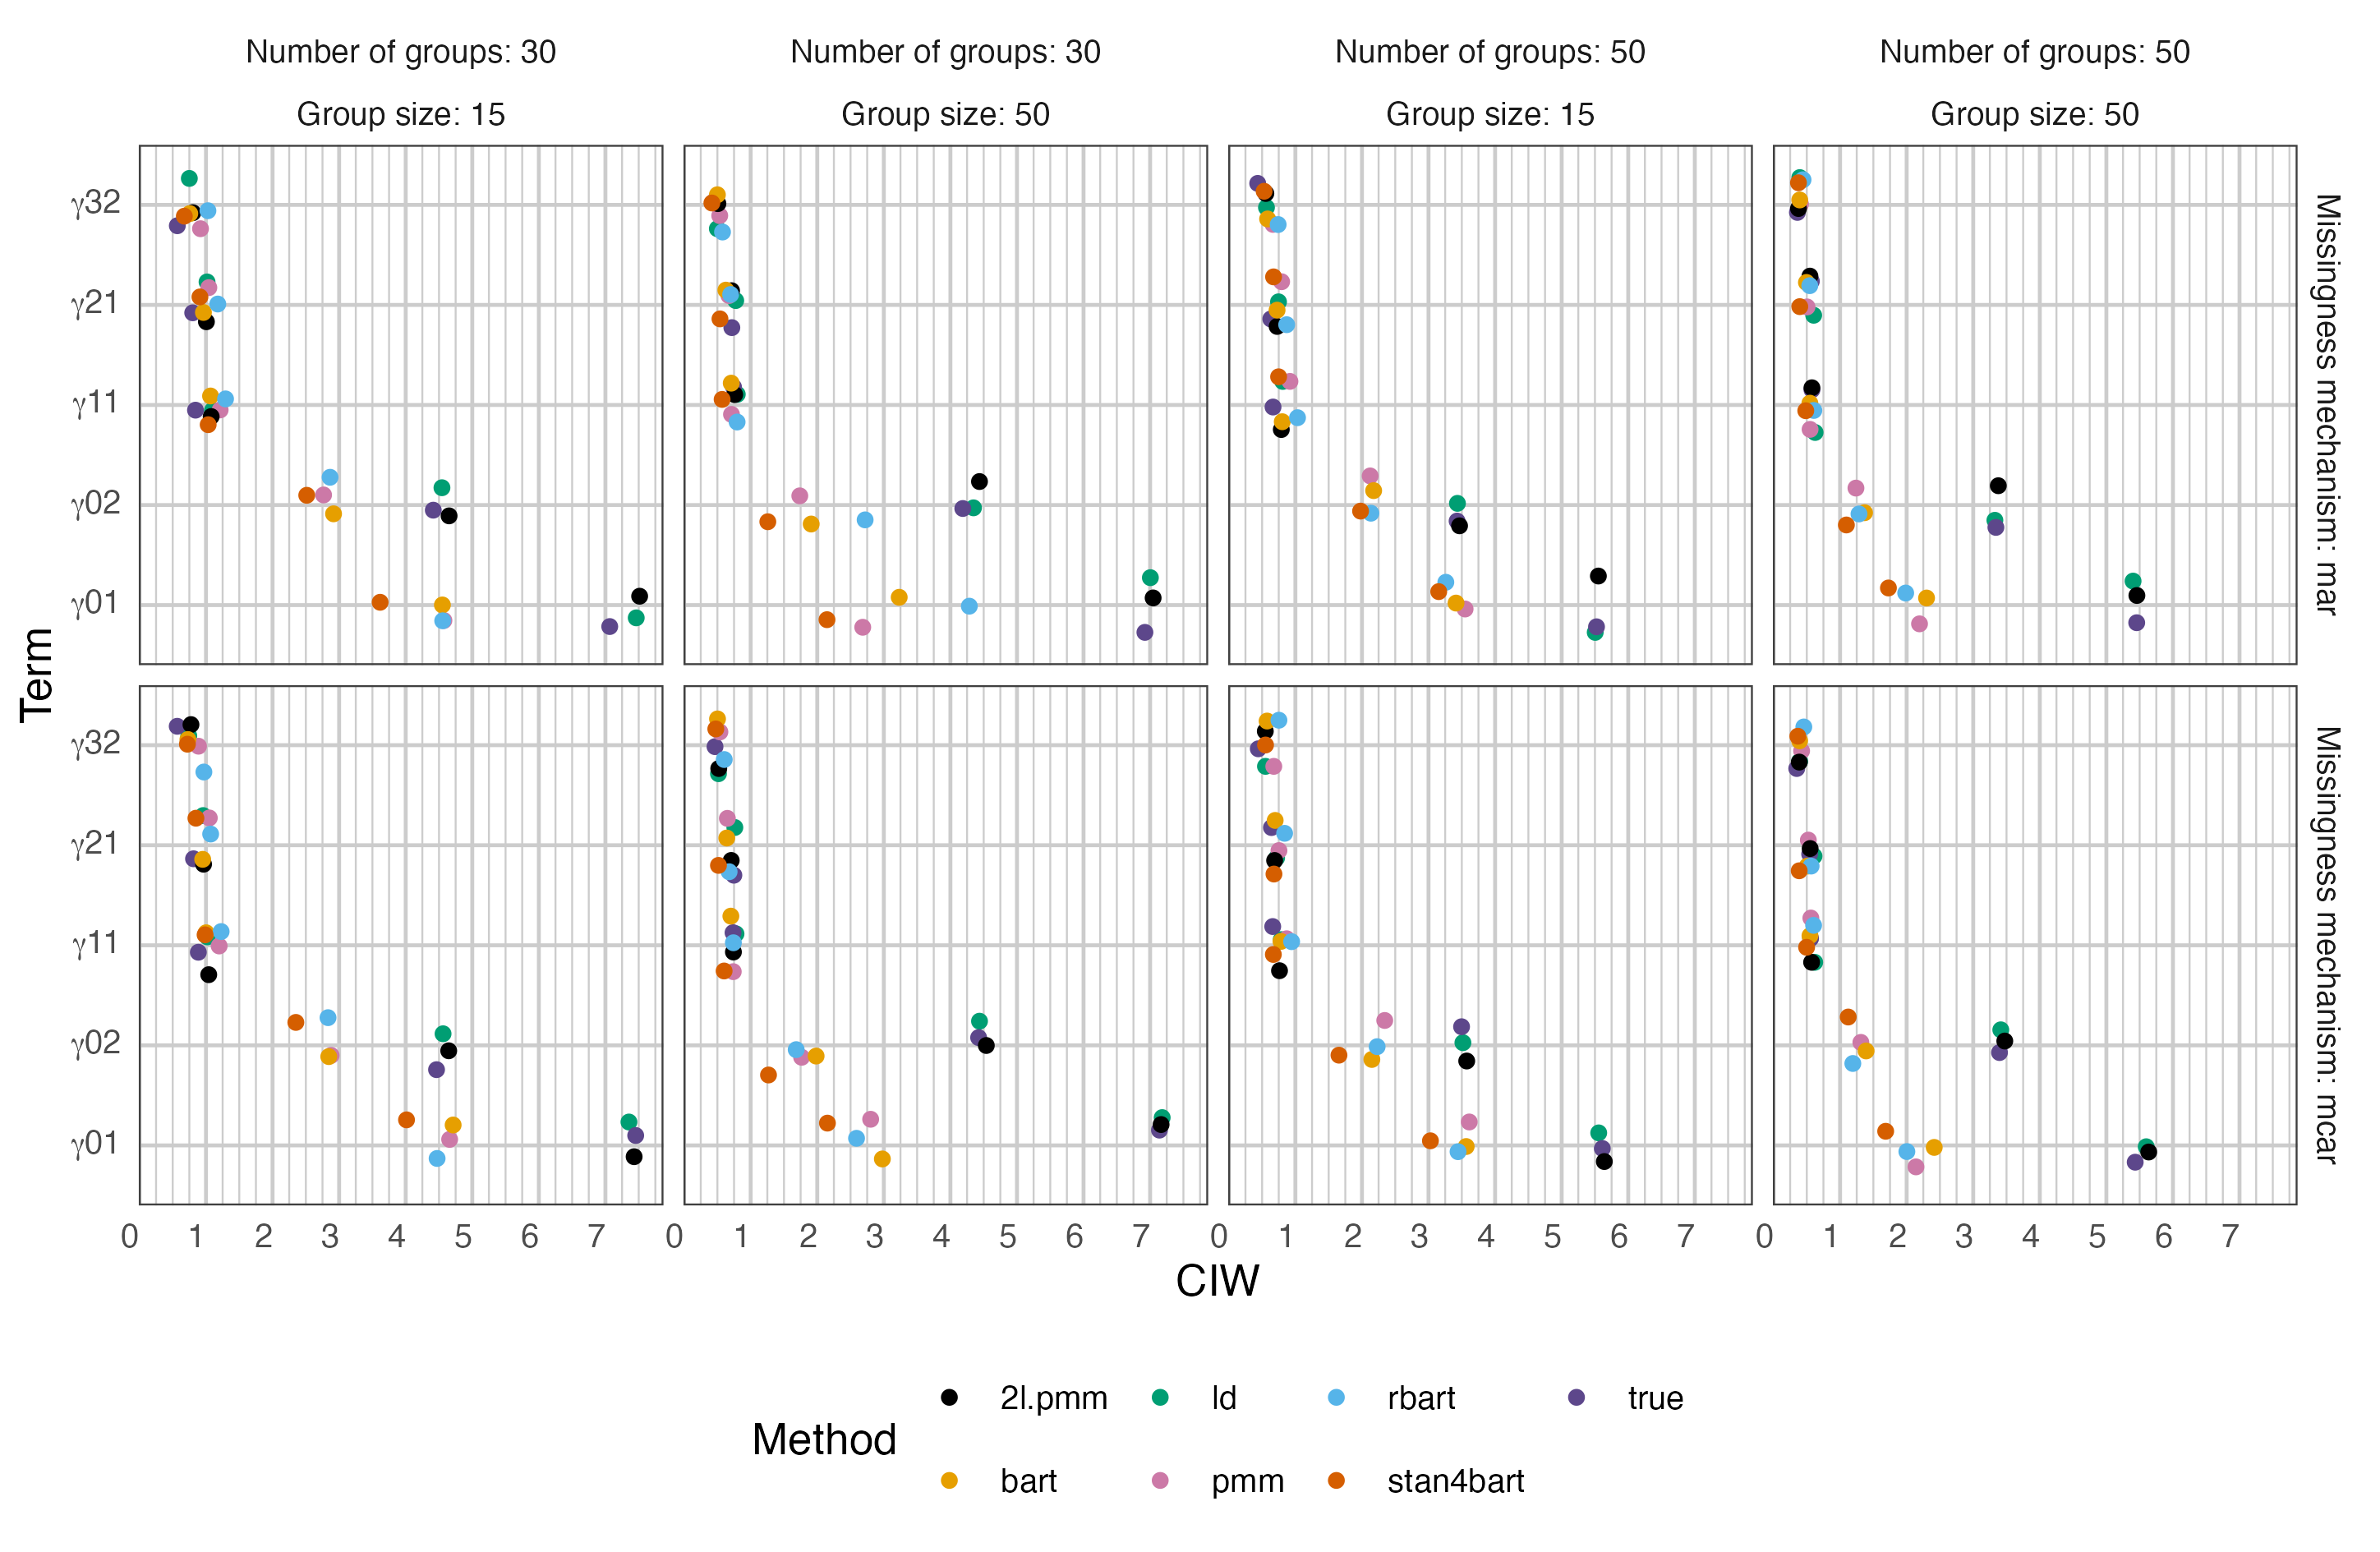
\includegraphics[width=1\textwidth]{ciwlevel2.png}
%     \caption{Confidence interval width of the estimates}
%     \label{fig:ciwlevel2}
% \end{figure}

The width of the 95\% confidence intervals for the cross-level interactions --- shown in figure \ref{fig:ciwcrosslevel} show a similar pattern for all methods: when group sizes are 15, all methods have confidence intervals larger than the 0\% missing data. However, when group sizes are 50, the confidence intervals decrease in size for all methods, either being smaller than or similar to the 0\% missing data. This pattern is also reflected in figure \ref{fig:coveragelevel2}, where these smaller intervals result in undercoverage.

\begin{figure}[H]
    \centering
    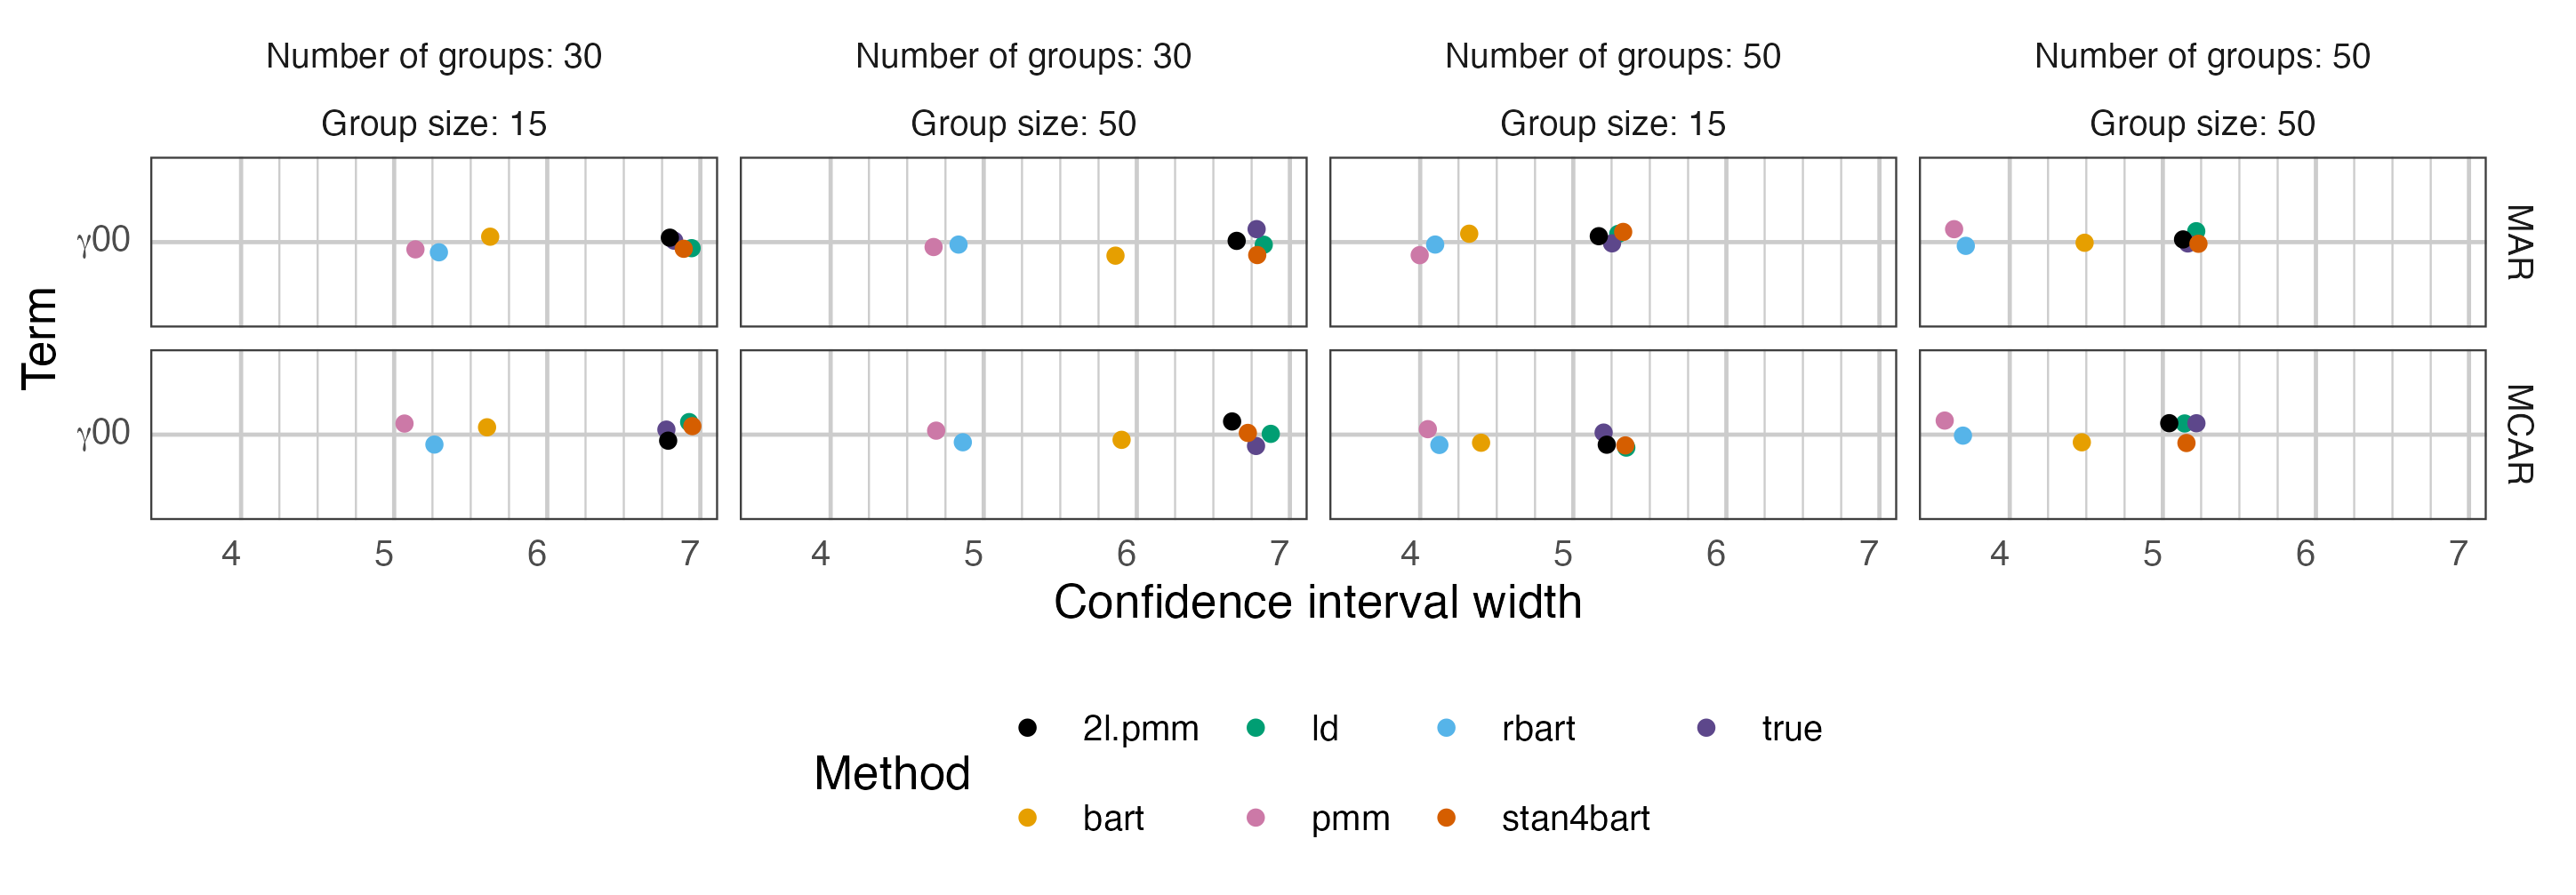
\includegraphics[width=1\textwidth]{ciwintercept.png}
    \caption{Width of the 95\% confidence intervals for the intercept of the linear mixed model for all simulated datasets over 100 simulations with ICC = .5.}
    \label{fig:ciwintercept}
\end{figure}

\begin{figure}[H]
    \centering
    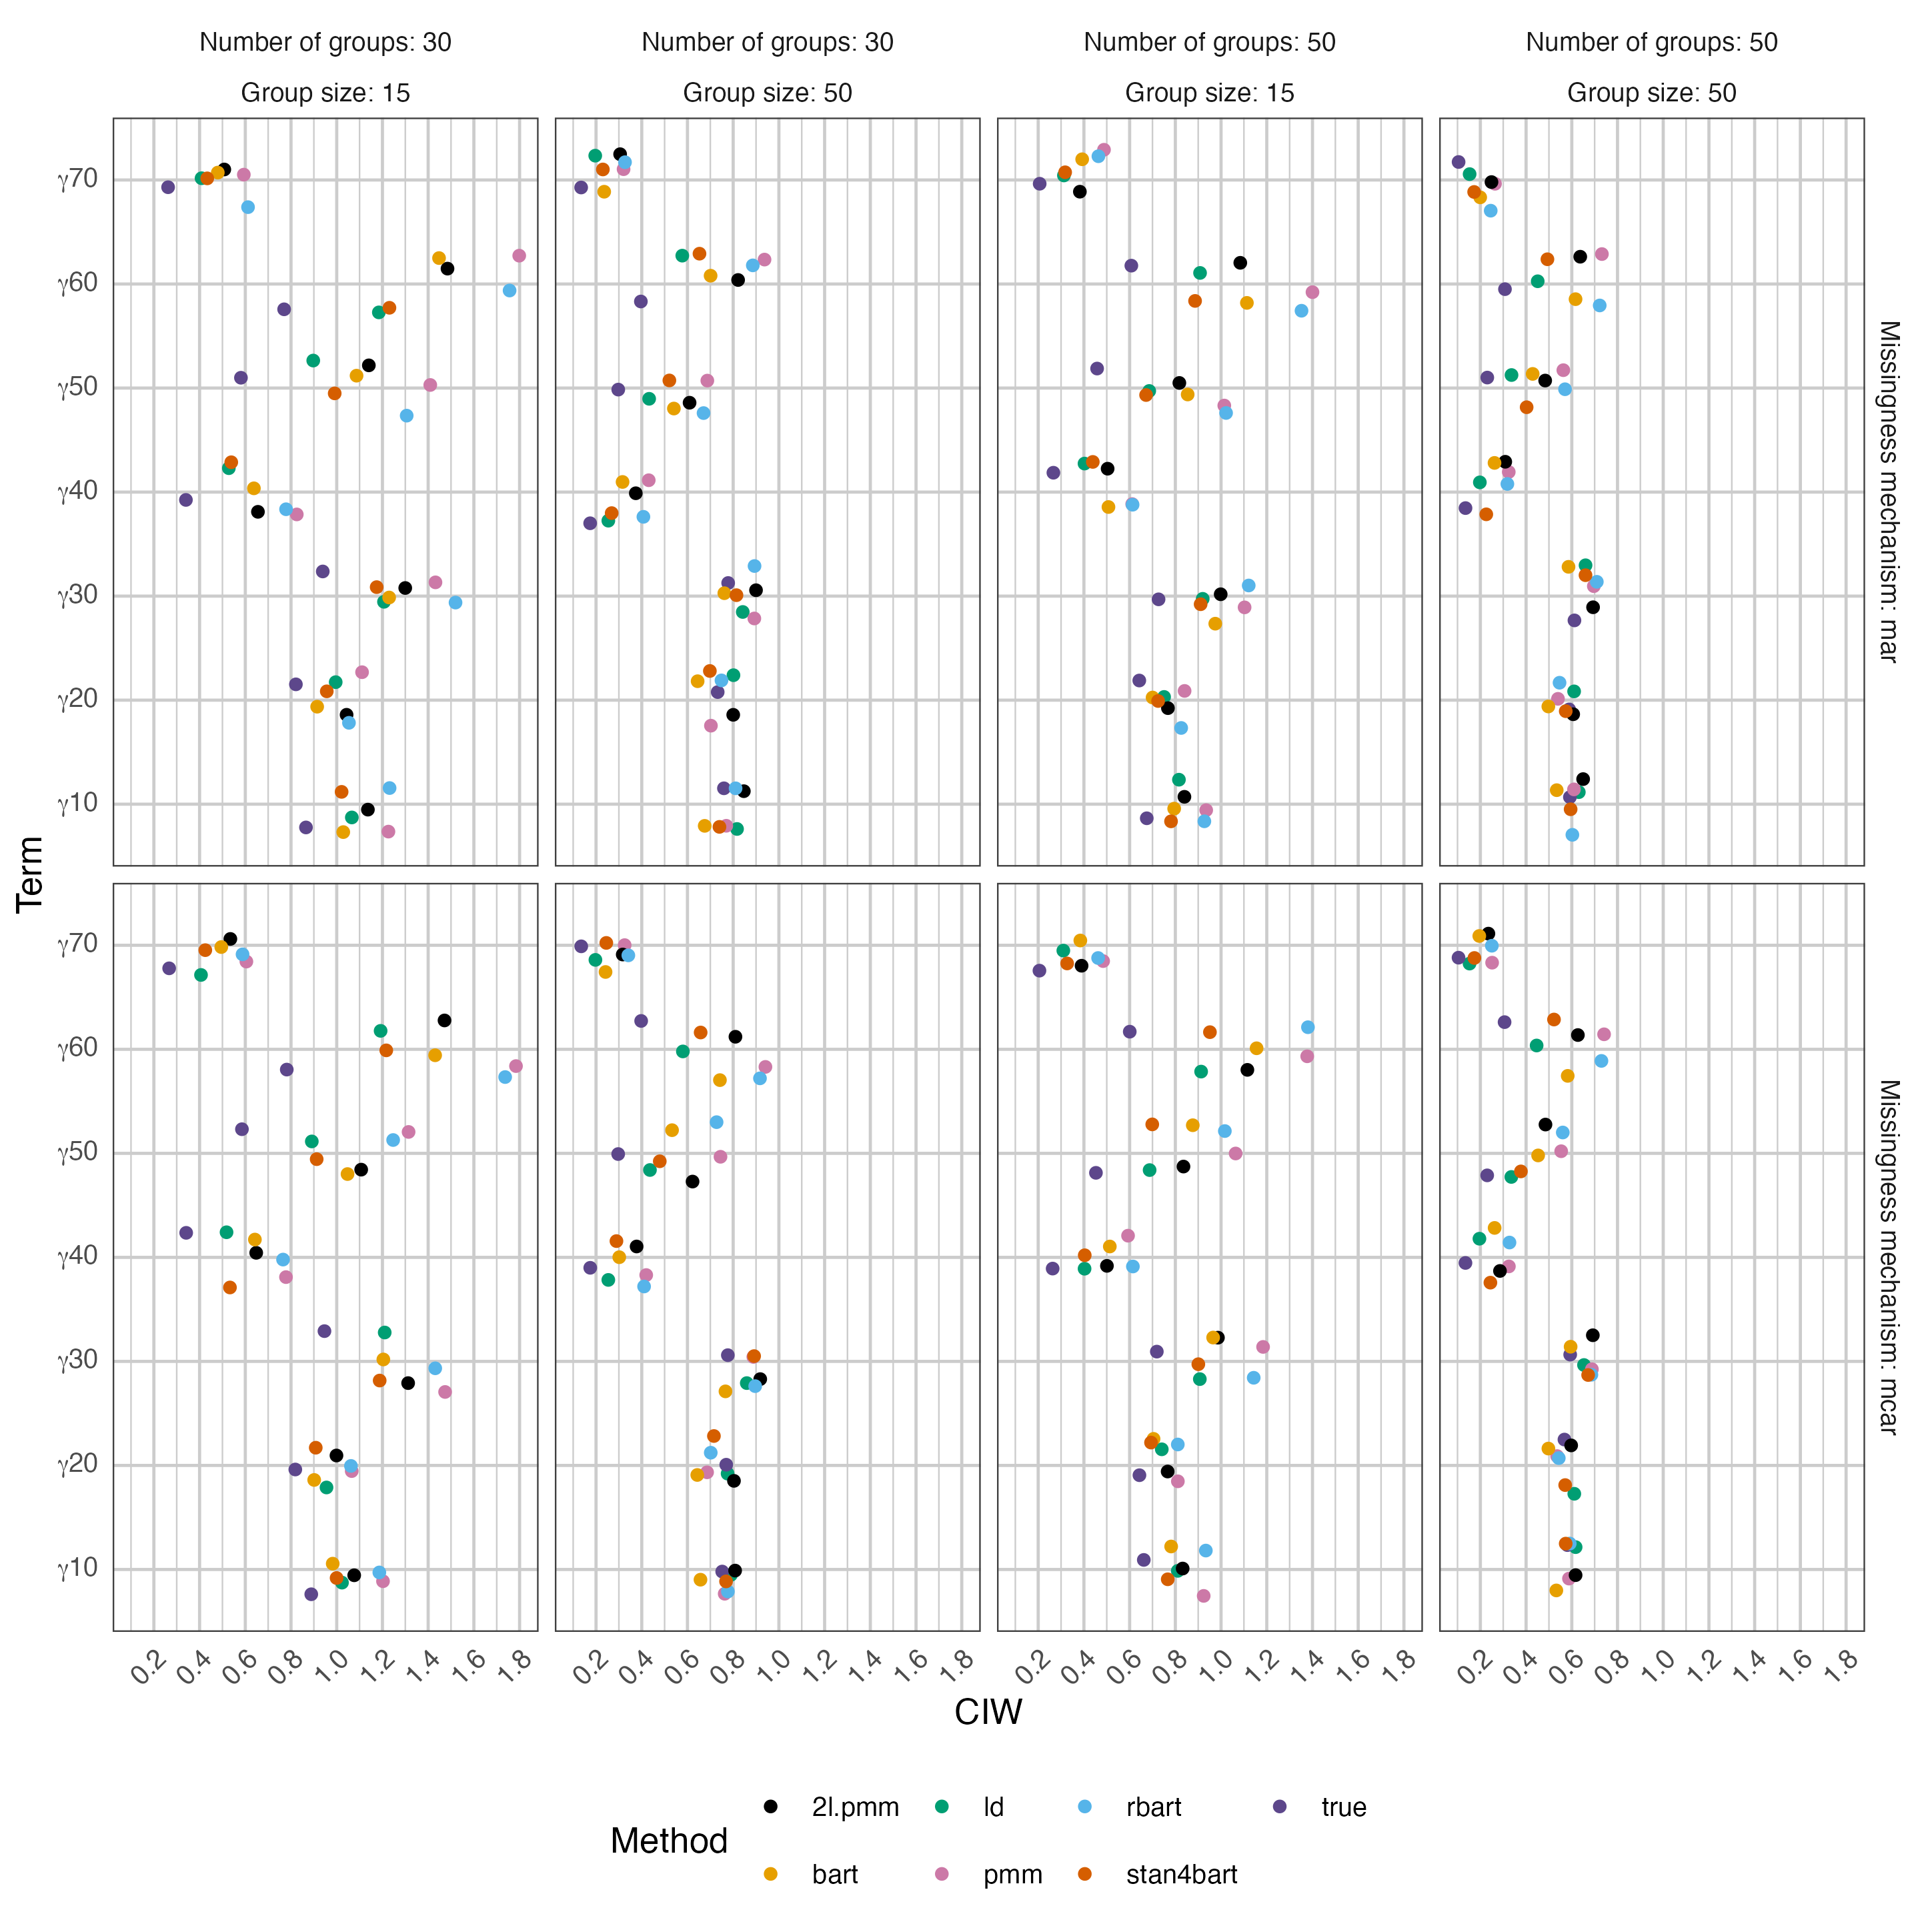
\includegraphics[width=1\textwidth]{ciwlevel1.png}
    \caption{Width of the 95\% confidence intervals for the level-1 effects of the linear mixed model for all simulated datasets over 100 simulations with ICC = .5.}
    \label{fig:ciwlevel1}
\end{figure}

\begin{figure}[H]
    \centering
    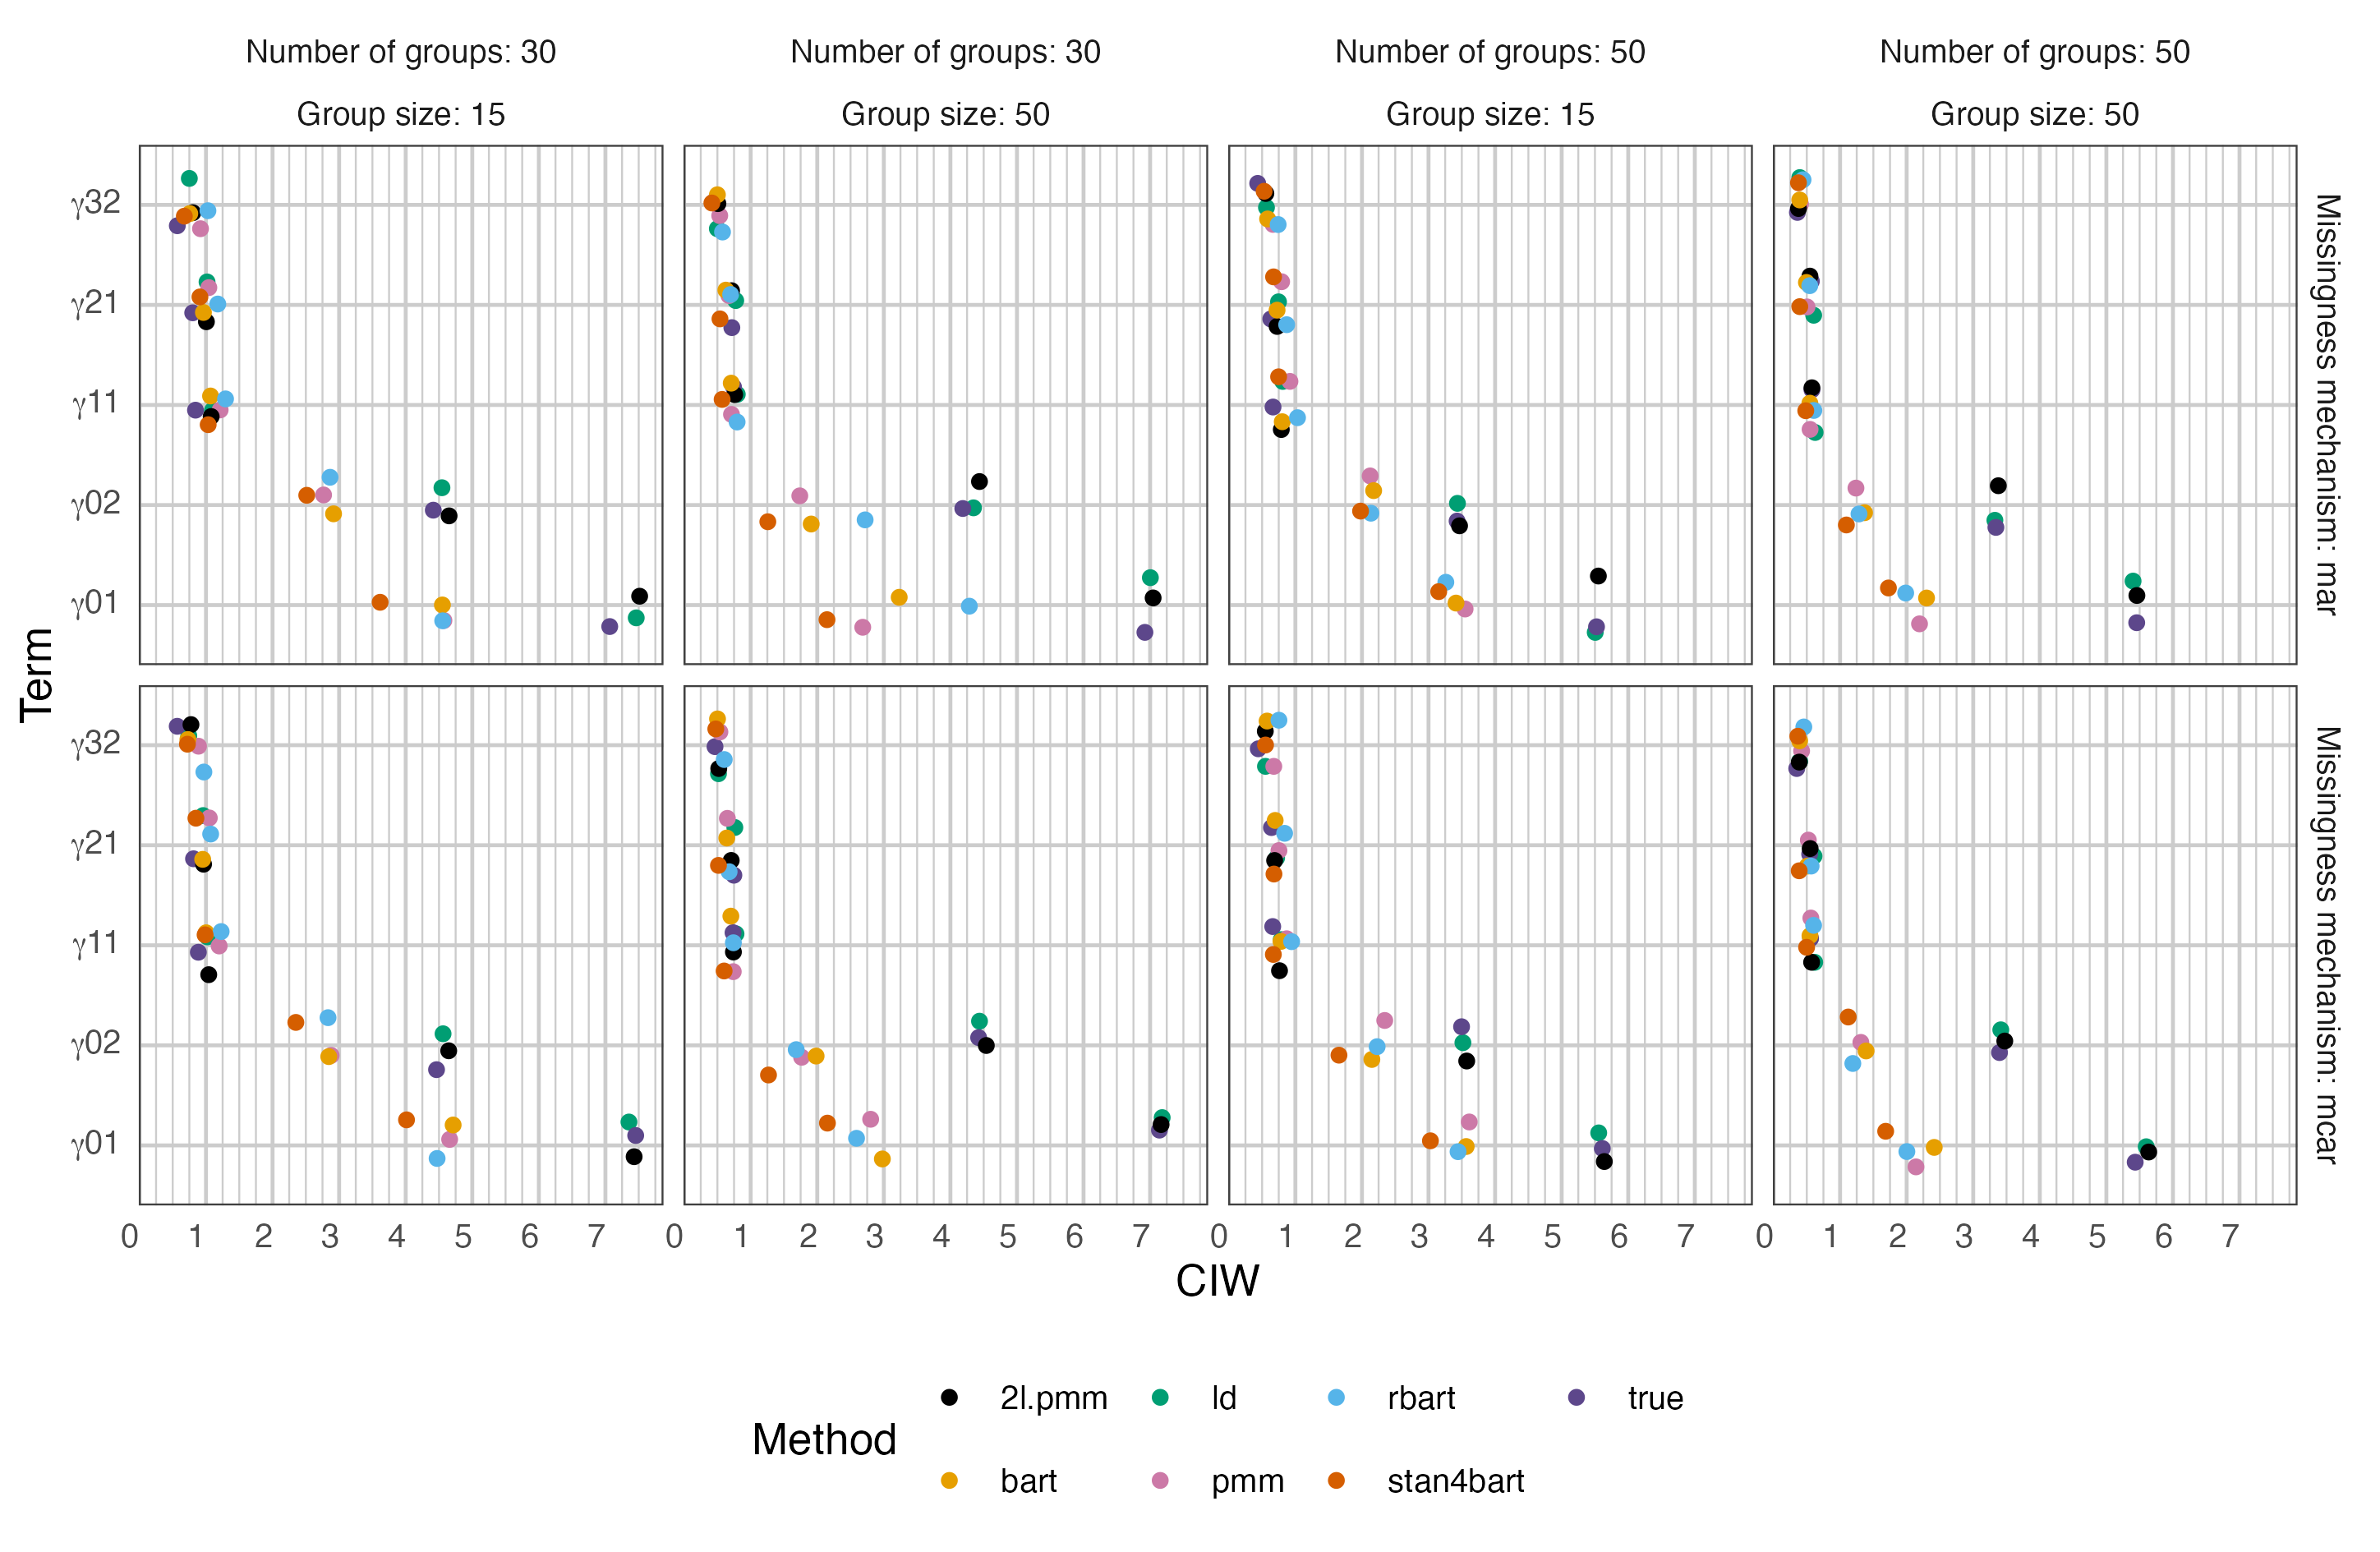
\includegraphics[width=1\textwidth]{ciwlevel2.png}
    \caption{Width of the 95\% confidence intervals for the level-2 effects of the linear mixed model for all simulated datasets over 100 simulations with ICC = .5.}
    \label{fig:ciwlevel2}
\end{figure}

\begin{figure}[H]
    \centering
    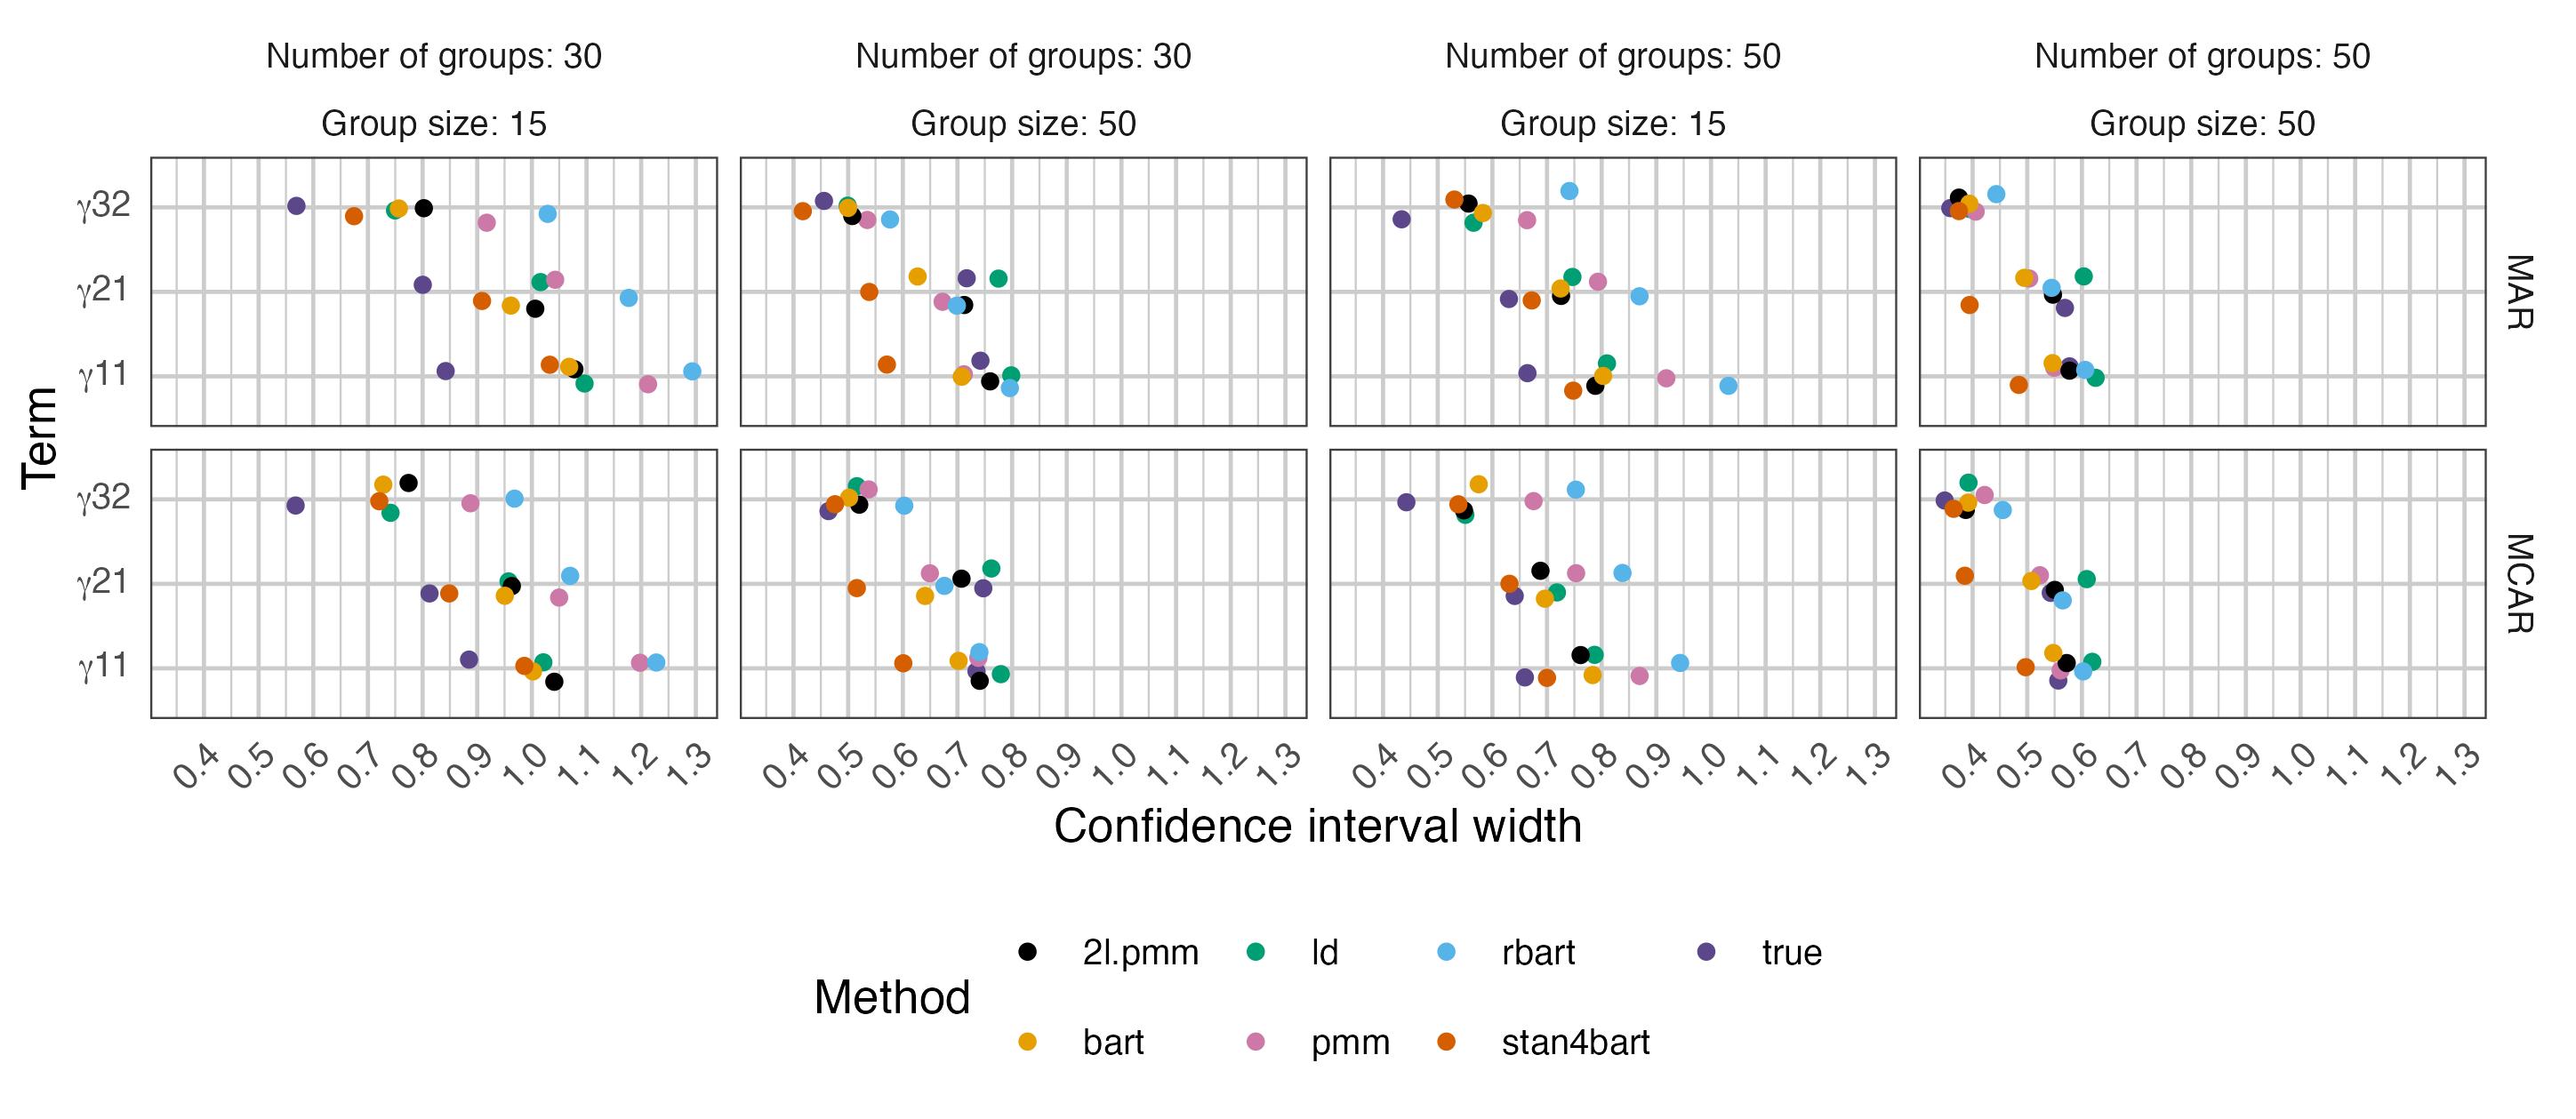
\includegraphics[width=1\textwidth]{ciwcrosslevel.png}
    \caption{Width of the 95\% confidence intervals for the cross-level interaction effects of the linear mixed model for all simulated datasets over 100 simulations with ICC = .5.}
    \label{fig:ciwcrosslevel}
\end{figure}

\section{Discussion}
% \begin{enumerate}
%     \item Short reiteration of research problem
%     \item Interpretation of results
%     \begin{enumerate}
%         \item overall best performance of 2l.PMM 
%         \item Performance PMM and BART as expected --> unable to capture multilevel structure of the data 
%         \item overall worst performance of method R-BART
%         \item R-BART really bad in intercept variance, fixed effects, level-2 effects, cross-level, residual variance, random slopes ---> at times performing even worse than BART. Would be interesting to see how it would perform if there are no random slopes in the data, thus only random intercepts (which it is supposedly modelling). 
%         \item Listwise deletion performs really good, even under MAR which is surprising ---> might be modelling a special case. 
%         \item stan4bart has an okay performance. Certainly one that hopefully spraks interest. It performs badly in level-2 effects (fixed and cross-level), however it might be interesting how this would perform with including passive imputation (?? dont know if that is even possible). However, this would make the imputation method more complex and less user-friendly --> it would look very similar to the imputation method 2l.PMM in terms of specification. stan4bart does outperform 2l.PMM in terms of random effects and residual variance. one big downside of this method was the computational time (loop 4 took around 3 days to run).
%     \end{enumerate}
%     \item comparison with previous research 
%     \item limitations of this study
%     \begin{enumerate}
%         \item 100 repetitions, sometimes 20
%         \item computational time 
%         \item not many different factors
%         \item matching method 
%     \end{enumerate}
%     \item future research recommendations
%     \begin{enumerate}
%         \item interesting explorations for stan4bart: reduce computational time, matching procedure for predictive mean matching, passive imputation, MAR and MCAR, different amount of missingness, different effect sizes, smaller sample sizes.
%     \end{enumerate}
% \end{enumerate}

The goal of this study was to investigate whether the use of multilevel BART models in MI could improve its performance in the context of missing multilevel data. Even though MI has been implemented in a multilevel context \citep{mistlerComparisonJointModel2017, enders2018, enders2018a, enders2020, buurenFlexibleImputationMissing2018, taljaard2008, enders2016, resche-rigon2018, audigier2018, dong2023, grund2016, grund2018a, grund2018, ludtke2017, grund2021, quartagno2022}, issues rise with the current implementation. Since MLMs are build step-wise with non-linearities, ensuring congeniality between the imputation model and analysis model is difficult. Additionally, mimicking the hierarchical structure of the data in the imputation models is also challenging \citep{buurenFlexibleImputationMissing2018, burgette2010, hox2011} and can result in complex models that might not converge \citep{buurenFlexibleImputationMissing2018}. So, this study aimed to solve these problems by using non-parametric, tree-based models in the imputation process. These models are able to implicitly model non-linearities and interactions \citep{hill2020, burgette2010, lin2019, chipman2010, james2021, salditt2023, breiman1984}, possibly alleviating the problems when defining a multilevel imputation model. 

The results indicate that out of all imputation methods, the conventional multilevel imputation method --- 2l.PMM --- had the best overall performance. On average, it showed the least overall bias and most consistent coverage. Furthermore, the width of its confidence intervals oftentimes mimicked that of the ``ture'' data with 0\% missing. On the other hand, the random effects --- i.e. the random slopes, random intercept, and residual variance --- were often biased for the 2l.PMM. Furthermore, some coverage estimates for the fixed effects suggested some efficiency could still be gained. % add stuff about biased interactions via passive imputation.

Unsurprisingly, single-level imputation methods --- PMM and BART --- were unable to accurately capture the multilevel structure of the data: underestimating level-2 effects, cross-level interactions and the random structure of the data, while still showing acceptable results for the overall intercept and level-1 effects. The undercoverage of the overall intercept and level-1 effects $\gamma_{10}, \gamma_{20}$ and $\gamma_{30}$ as well as their inaccurate confidence interval widths are in line with prior research showing that ignoring the multilevel structure results in underestimating the ICC, standard errors, random intercepts, random slopes, and overestimating the residual variance \citep{buurenFlexibleImputationMissing2018, ludtke2017, taljaard2008, hox2011,enders2016}.

Most surpising was the performance of R-BART, which is a model that should be able to account for some random structure in the data --- namely, random intercetpts. However, looking at the results, it had the worst overall performance. Remarkably, it was unable to capture the random intercept in the data --- greatly underestimating it. Moreover, R-BART only showed acceptable results for some --- not all --- fixed level-1 effects and was being outperformed by BART at times. However, the model developed by \citet{wagner2020,tan2016} and \citet{dorie2024} was only evaluated by them under a model without random slopes in a prediction context showing promising results. So, it would be interesting to evaluate this imputation method with a model that only includes random intercepts, to see if it would perform better. % stan4bart paper did compare  this, but unclear what the estimand is in that paper.

Together with 2l.PMM, stan4bart was a model that could incorporate the most multilevel structure present in the data. While showing some promising results, stan4bart also showed some considerable biases and undercoverages. It seemed to have the most trouble with the level-2 effects --- fixed level-2 effects and cross-level effects. However, it did show the best performance in terms of the random structure of the data, outperforming 2l.PMM. Still, a major disadvantage of this method is its exstensive computational time: the imputation of a dataset with 50 groups of size 50 took around 3 days to complete. % also consider the stan4bart paper? but estimand may be very different from my evaluations.

Lastly, listwise deletion showed even better results than expected: it out performed 2l.PMM routinely for almost all parameters. This would be expected under MCAR but not under MAR \citep{buurenFlexibleImputationMissing2018,enders2018a,peeters2015,austin2021,carpenter2013,little2002,grund2018,ludtke2017,grund2021,schouten2021}. Thus, these results seem to indicate that a special case was generated, resulting in listwise deletion outperforming the other imputation methods when the missing data was generated as MAR. % investigate the possible special case.

This study had a few limitations. Firstly, due to time restrictions paired with exstensive computational time necessary for the imputation methods, only 100 repetitions were used to evaluate the methods. As a result, especially 95\% confidence interval coverage estimates might be less reliable.~\citet{morris2019} define a minimum of repetitions in a simulation study based on the required level of precision --- MCSE --- and expected coverage. For an  MCSE of 0.5\% and expected coverage of 95\%, they pose that 1900 repetitions are needed. Secondly, in their current implementation, the BART imputation models --- single-level BART, R-BART and stan4bart --- are computationally expensive; taking, at the least, several hours to impute one dataset. Then, this study considered a limited amount of factors. For example, the amount of missingness was fixed at 50\% and the ICC was fixed at 0.5, resulting in a possbly limited picture of the performance of the imputation methods. Since, the amount of missingness and the ICC can greatly influence the performance of the imputation methods \citep{enders2018,enders2018a,enders2020,mistler2017,akkayahocagil2023,grund2016,grund2018a,grund2018,ludtke2017,grund2021}. Furthermore, as mentioned above, the generated MAR mechanism did not mimic the expected characteristic associated with MAR. So, the performance of the imputation methods were not evaluated under a true MAR mechanism, which is common when evaluating imputation methods \citep{buurenFlexibleImputationMissing2018,enders2018a,peeters2015,austin2021,carpenter2013,little2002,grund2018,ludtke2017,grund2021,schouten2021} as well as important because, in real-life data, MCAR can rarely be assumed \citep{oberman2023,buurenFlexibleImputationMissing2018,kang2013,little2002}.

So, avenues for future research include exploring the performance of the multilevel BART model --- stan4bart --- under a true MAR mechanism, or, additionally a MNAR mechanism, which \citet{oberman2023} pose to be a likely real-life missingness mechanism. Thus, for a method to perform well in real-life situations, it should preferrably performs well under both MAR and MNAR \citep{oberman2023}. Furthermore, the performance of stan4bart could be evaluated under different amounts of missingness, different ICCs, and more different nunmber of groups and group sizes to reflect other realistic sitations. For example, group sizes of 5 are often found in family-type research \citep{maas2005}. Also, research could be conducted into the reduction of computational time for stan4bart. Research could look into the effect of reducing the number of posterior samples, thinning samples, burn-in samples or other specifications for the stan4bart method. Then, lastly, the matching procedure for the predictive mean matching in the stan4bart method could be explored. Research could examine how different matching methods \citep{buurenFlexibleImputationMissing2018} could be implemented and how they would affect the performance of the stan4bart method.

\section{Conclusion}

To sum up, this study aimed to alleviate the complexities associated with mulitple imputation in a multilevel context by using BART models as the imputation models. Being non-parametric and tree-based, BART models were expected make defining a congenial and well performing imputation model for multilevel data easier. However, the current implementation of a multilevel BART imputation method did not improve on the current implementation of multilevel predictive mean matching. Meanwhile, also showing inviting results for future research into the multilevel BART imputation method.

\newpage
\bibliography{thesis}
\addcontentsline{toc}{section}{References}
\bibliographystyle{apalike}

\newpage
\appendix
\section{Imputation functions} \label{appendix:imputationfunctions}
\subsection{Single-level BART}
\begin{lstlisting}[language=R, caption = {Imputation function for single-level BART}, label = {lst:singlelevelBART}]
    mice.impute.bart <- function(y, ry, x, wy = NULL, use.matcher = FALSE, donors = 5L, ...) {
        install.on.demand("dbarts", ...)
        if (is.null(wy)) {
            wy <- !ry
        }
    
        # Parameter estimates
        fit <- dbarts::bart(x, y, keeptrees = TRUE, verbose = FALSE)
    
        yhatobs <- fitted(fit, type = "ev", sample = "train")[ry]
        yhatmis <- fitted(fit, type = "ev", sample = "train")[wy]
    
        # Find donors
        if (use.matcher) {
            idx <- matcher(yhatobs, yhatmis, k = donors)
        } else {
            idx <- matchindex(yhatobs, yhatmis, donors)
        }
    
        return(y[ry][idx])
    }
\end{lstlisting}
\subsection{Random intercept BART}
\begin{lstlisting}[language=R, caption={Imputation function for random intercept BART}, label={lst:randominterceptBART}]
    mice.impute.2l.rbart <- function(y, ry, x, wy = NULL, type, use.matcher = FALSE, donors = 5L, ...) {
        install.on.demand("dbarts", ...)
        if (is.null(wy)) {
            wy <- !ry
        }
    
        clust <- names(type[type == -2])
        effects <- names(type[type != -2])
        X <- x[, effects, drop = FALSE]
    
        model <- paste0(
            "y ~ ", paste0(colnames(X), collapse = " + ")
        )
    
        fit <- dbarts::rbart_vi(formula = formula(model), group.by = clust, data = data.frame(y, x), verbose = FALSE, n.threads = 1, n.samples = 500L, n.burn = 500L, ...)
    
        yhatobs <- fitted(fit, type = "ev", sample = "train")[ry]
        yhatmis <- fitted(fit, type = "ev", sample = "train")[wy]
    
        # Find donors
        if (use.matcher) {
            idx <- matcher(yhatobs, yhatmis, k = donors)
        } else {
            idx <- matchindex(yhatobs, yhatmis, donors)
        }
    
        return(y[ry][idx])
    }
\end{lstlisting}
\subsection{Multilevel BART}
\begin{lstlisting}[language=R, caption={Imputation function for multilevel BART with random effects and cross-level interactions}, label={lst:multilevelBART}]
    mice.impute.2l.bart <- function(y, ry, x, wy = NULL, type, intercept = TRUE, use.matcher = FALSE, donors = 5L, ...) {
        install.on.demand("stan4bart", ...)
        if (is.null(wy)) {
            wy <- !ry
        }
    
        if (intercept) {
            x <- cbind(1, as.matrix(x))
            type <- c(2, type)
            names(type)[1] <- colnames(x)[1] <- "(Intercept)"
        }
    
        clust <- names(type[type == -2])
        rande <- names(type[type == 2])
        fixe <- names(type[type > 0])
    
        lev <- unique(x[, clust])
    
        X <- x[, fixe, drop = FALSE]
        Z <- x[, rande, drop = FALSE]
        xobs <- x[ry, , drop = FALSE]
        yobs <- y[ry]
        Xobs <- X[ry, , drop = FALSE]
        Zobs <- Z[ry, , drop = FALSE]
    
        # create formula
        fr <- ifelse(length(rande) > 1,
            paste0("+ (1 +", paste(rande[-1L], collapse = "+")),
            " + (1 "
        )
        randmodel <- paste0(
            "y ~ bart(", paste0(fixe[-1L], collapse = " + "), ")",
            fr, "| ", clust, ")"
        )
    fit <- eval(parse(text = paste("stan4bart::stan4bart(", randmodel,
        ", data = data.frame(y, x),
            verbose = -1,
            bart_args = list(k = 2.0, n.samples = 500L, n.burn = 500L, n.thin = 1L, n.threads = 1))",
        collapse = ""
    )))
    
        yhatobs <- fitted(fit, type = "ev", sample = "train")[ry]
        yhatmis <- fitted(fit, type = "ev", sample = "train")[wy]
    
        # Find donors
        if (use.matcher) {
            idx <- matcher(yhatobs, yhatmis, k = donors)
        } else {
            idx <- matchindex(yhatobs, yhatmis, donors)
        }
    
        return(y[ry][idx])
    }
\end{lstlisting}

\section{Appendix B}

\end{document}

